\documentclass{cacthesis}
\usepackage{tabularx}
\usepackage{caption}
\usepackage{listings}
\usepackage{xcolor}
\usepackage{pifont}% http://ctan.org/pkg/pifont
\usepackage{amssymb}% http://ctan.org/pkg/amssymb
\usepackage{mdframed}
\usepackage{dsfont}
\usepackage{amsthm}
\usepackage{bm}
\usepackage{algorithm}
\usepackage{algpseudocode}
\usepackage{bbm}
\usepackage{hyperref}
\usepackage{amsmath,amssymb}
\usepackage{todonotes}
\usepackage{subcaption} % For subfigures with their own captions
\usepackage[
backend=biber,
style=alphabetic,
sorting=ynt
]{biblatex}
\addbibresource{bibliography.bib}

\newtheorem{theorem}{Theorem}
\newtheorem{construction}{Construction}

\newenvironment{specialconstruction}[1]
  {% Before code
   \refstepcounter{construction}% Increment the construction counter
   \begin{mdframed}
   \noindent\textbf{Construction \theconstruction: #1}\par
  }
  {% After code
   \end{mdframed}
  }


\newcommand{\cmark}{\ding{51}}%
\newcommand{\xmark}{\ding{55}}%

\newcounter{protocol}
\newenvironment{protocol}[1]
  {\par\addvspace{\topsep}
   \noindent
   \tabularx{\linewidth}{@{} X @{}}
    \hline
    \refstepcounter{protocol}\textbf{Protocol \theprotocol} #1 \\
    \hline}
  { \\
    \hline
   \endtabularx
   \par\addvspace{\topsep}}

\newcommand{\sbline}{\\[.5\normalbaselineskip]}% small blank line
\newtheorem{definition}{Definition}

\begin{document}

	\frontmatter
	
	%%%%%%%%%%%%%
	%% Title page
	%%%%%%%%%%%%%
	\title{Implementation and Evaluation of Pseudorandom Correlation Generators in the Context of Threshold BBS+}
	\author{Leandro Rometsch}
	\date{April 08, 2024}
	\subject{Master Thesis}
	
	\publishers{
		\small
		\begin{tabular}{r l}
			Supervisors: &  Prof. Sebastian Faust, Ph.D. & & David Kretzler & & Benjamin Schlosser
		\end{tabular}
	}
	\maketitle
        \section*{Abstract}
Secure multi-party computation (MPC) protocols often employ correlated randomness to improve efficiency and benefit from this by separating their operations into a computationally intensive preprocessing (offline) phase and a highly efficient, non-interactive (online) phase. This trade-off is especially valuable in setups with high latency, such as when participants are geographically dispersed. By making the online phase non-interactive, the otherwise costly rounds of communication are eliminated. In addition, it allows parties to utilize previously unused idle time for preprocessing in order to speed up the time-critical, input-dependent part of their protocol. Pseudorandom correlation generators (PCG), introduced by Boyle et al. \cite{boyle2019efficient, boyle2020efficient}, facilitate the preprocessing approach by extending short correlated seeds into long instances of a target correlation. In particular, the primitive allows seed generation with sublinear communication complexity, while the extension can be performed locally, making the preprocessing phase practical compared to previous approaches. Despite their theoretical value and use in various MPC protocols, PCG implementations have been lacking. 

This work addresses this by presenting practical considerations for implementing the PCG construction by Boyle et al. \cite{boyle2020efficient}. We demonstrate the value of these optimizations within the offline phase of Faust et al.'s non-interactive threshold BBS+ signature scheme \cite{faust2023non}. Our implementation is the first to support the threshold setting and achieves quasilinear runtime for the number of presignatures generated, with linear runtime increasing for the number of participants. We provide benchmarks for up to $10$ parties and find that in the $2$-out-of-$2$ setting, our PCG generates $2^{17}$ presignatures in $100$ms per presignature while adding around $80$ms per additional party. Our implementation significantly outperforms ($6$x to $10$x) the only other available PCG implementation for threshold ECDSA \cite{abram2022low} while incorporating an additional correlation.
        
	\tableofcontents
	    
	\mainmatter
	
        \chapter{Introduction}
Correlated secret randomness is considered to be a useful resource for enhancing both the performance and security of secure multi-party computation (MPC) protocols \cite{ishai2013power}. The type of correlation determines the kind of MPC circuit supported; for example, oblivious transfer (OT) correlations work with boolean circuits \cite{goldreich2019play}, while oblivious linear-function evaluation (OLE) is used for arithmetic circuits \cite{ishai2009secure}. In order to get correlated secret randomness there is usually a distribution phase. In this phase, each party receives a sample from a joint random distribution. Although the samples are random, they adhere to the specified correlation. MPC protocols utilizing correlated secret randomness are therefore split up into an input-independent \textit{offline} and input-dependent \textit{online phase}. This is commonly referred to as \textit{preprocessing}, since the offline phase generates many instances of the required correlation, which are then consumed by the online phase. The approach has the potential to make the online phase very efficient by shifting communication and computationally demanding tasks to the offline phase. Preprocessing is therefore very appealing for real-world applications, since it enables participants to utilize their idle times to speed up the critical (on-demand) part of their MPC protocol.
\\\\
In recent years, Boyle et al. proposed \cite{boyle2015function} and further refined \cite{boyle2016function, boyle2020efficient} the novel primitive of a pseudorandom correlation generator (PCG), which provides a promising approach for the realization of a preprocessing phase. A PCG can be thought of as a form of (distributed) pseudorandom generator in which participants generate seeds and then locally expand them for pseudorandom bit streams. Crucially, the PCG expansion ensures that the generated bit streams are correlated across participants. Such a primitive provides several advantages to the preprocessing model: On the one hand, it reduces offline communication because seed expansion is done locally. It also reduces storage costs, since the correlations are compressed in the PCG seed and the parties can decide to expand them only when needed. Furthermore, only the seed generation needs to be protected against malicious parties, since malicious seed expansion does not effect honest parties.
\\\\
This work implements and evaluates an efficient \texttt{Ring-LPN}-based PCG construction proposed by Boyle et al. in \cite{boyle2020efficient}. The construction is of high practical relevance since it avoids the quadratic complexity of previous approaches. The PCG realizes OLE and Vector-OLE correlations, but the general approach can be modified to produce multiplication and authentication triples.


\\\\
% BBS+
Multi-Party Computation (MPC) is commonly used in modern cryptographic schemes, enabling multiple parties to jointly compute a function over their inputs while keeping those inputs private. An important concept within MPC is correlated secret randomness, a mechanism that, despite its simplicity, significantly enhances the efficiency and feasibility of lightweight MPC protocols, especially in scenarios lacking an honest majority. Correlated randomness, such as oblivious transfer and multiplication triples, underpins secure computation by pre-establishing secret, shared structures that simplify and streamline the online computation phase.
\\\\
The preprocessing model emerges as a natural evolution in the pursuit of practical MPC, addressing the inherent challenges of real-time computation under stringent security requirements. Within this model, the concept of Pseudorandom Correlation Generators (PCGs) introduces a groundbreaking approach. PCGs enable parties to generate a compact seed in a setup phase that can later be expanded into a large volume of correlated randomness needed for secure computation, without further interaction. This paradigm not only promises to reduce the communication and computational overhead associated with traditional MPC protocols but also opens new avenues for efficiency and scalability in cryptographic designs.
\\\\
As an applied manifestation of these theoretical advancements, this work focuses on realizing PCGs for a specific non-interactive Threshold BBS+ scheme. The BBS+ signature scheme, lauded for its application in anonymous credential systems, stands out for its constant-size signatures over a set of attributes and its efficient protocols for both blind signing and selective disclosure. These features make BBS+ an invaluable tool in preserving privacy in digital interactions, where the ability to verify certain attributes without revealing a user's identity is increasingly crucial. By thresholding BBS+ signatures, we distribute the signing capability across multiple parties, eliminating single points of failure and enhancing security. Moreover, adopting a non-interactive approach during the signing phase significantly elevates the scheme's practicality, reducing latency and communication overhead in distributed environments.
\\\\
This work leverages the PCG framework proposed by Boyle et al., implementing it to produce the requisite correlated randomness for OLE and VOLE correlations. Subsequently, these implementations serve as the foundation for constructing a PCG for the BBS+ scheme, embodying a stride forward in the practical application of threshold cryptography and MPC in securing digital credentials. While Boyle et al. provided the theoretical blueprint, our contribution lies in bringing this vision to fruition, offering a tangible, efficient mechanism for generating correlated randomness that underpins a non-interactive, thresholded BBS+ signature scheme.

\section{Contribution}
\section{Related Work}
\section{Outline}

        \chapter{Preliminaries}

\textbf{Notation.} In this work, we denote the security parameter by $\lambda$ and the set $[k]$ as $\{0, ..., k-1\}$. We denote vectors in bold lower-case $\mathbf{v}$, matrices in bold upper-case $\mathbf{A}$, the tensor product of two vectors as $\mathbf{v}_0\otimes\mathbf{v}_0$, and the outer sum as $\mathbf{v}_0\boxplus\mathbf{v}_0$. We consider a degree-$n$ $\tau$-sparse vector to be a vector of dimension $n$ that contain $\tau$ non-zero elements. We consider a degree-$n$ $\tau$-sparse polynomial to be a polynomial of degree $n$ that contains $\tau$ non-zero coefficients.

\section{LPN-based Cryptography}
The Learning Parity with Noise (LPN) problem has emerged as a popular hardness assumption in several disciplines, including cryptography, machine learning, and coding theory. The basic concept of LPN is the difficulty of solving linear equations when they are contaminated with noise. This noise significantly increases the complexity of deriving accurate solutions, embodying the hardness of the assumption, which can be related to the NP-complete problem of \textit{decoding random linear codes} \cite{yu2016pseudorandom}. In the context of cryptography, the LPN assumption has found increasing application, particularly in the design of lightweight encryption and authentication schemes \cite{pietrzak2012cryptography}. Many of these applications are provably secure, meaning that any effective attack on such schemes would require overcoming the underlying LPN hardness assumption. In addition, LPN is gaining traction in post-quantum cryptography. Unlike other popular assumptions such as prime factorization and the discrete logarithm problem, which are vulnerable to quantum attacks via Shor's algorithm \cite{shor1999polynomial}, the LPN problem has not yet been efficiently solved by quantum algorithms \cite{zhao2018hardness}. 
In the following, we describe basic LPN and extend this description to LPN over rings with static leakage, which will serve as the main security assumption in this work.

\subsection{Primal- and Dual-LPN}
Primal Learning Parity with Noise (\texttt{Primal-LPN}) represents the foundational version of the LPN problem, offering adversaries black-box access to two oracles. The first oracle, containing a secret vector \( \mathbf{s} \in \mathbb{F}_2^{n} \), generates an error vector \( \mathbf{e} \in \mathbb{F}_2^{n} \) with each element independently derived from a Bernoulli distribution of probability \( \tau \). It then outputs a pair: a uniformly random matrix \( \mathbf{A} \in \mathbb{F}_2^{n\times n} \) and a vector \( \mathbf{t} = \mathbf{A}\mathbf{s} + \mathbf{e} \in \mathbb{F}_2^{n} \). The second oracle provides a uniformly random matrix \( \mathbf{A} \) and vector \( \mathbf{t} \), both in \( \mathbb{F}_2^{n\times n} \) and \( \mathbb{F}_2^{n} \) respectively, without the underlying \( \mathbf{s} \) and \( \mathbf{e} \) relationship. The adversary's task (in this decisional formulation of \texttt{Primal-LPN}) is to distinguish between pairs \((\mathbf{A}, \mathbf{t})\) that adhere to the linear equation \(\mathbf{t} = \mathbf{A}\mathbf{s} + \mathbf{e}\) and randomly generated pairs, which is computationally hard due to the obfuscating effect of the noise vector \( \mathbf{e} \) \cite{zhao2018hardness}. Notably, the problem description via Bernoulli implies that the problem remains hard for sparse noise vectors (i.e., containing a fixed number of zero elements) as proven by Liu et al. in \cite{liu2017hardness}. Notably, the \texttt{Primal-LPN} is equivalent to the \texttt{Dual-LPN} assumption \cite{couteau2021silver}, which provides a simplified representation of the LPN challenge. In this formulation, the secret is embedded within the linear transformation itself. The adversary now only needs to distinguish between a random matrix $H \in \mathbb{Z}_p^{m \times n}$ and the product $H \cdot \mathbf{e}$ for a noise vector $\mathbf{e}\in \mathbb{Z}_n^{m \times n}$.

\subsection{Ring-LPN}
\label{prelim:ring_lpn}
Ring Learning Parity with Noise (\texttt{Ring-LPN}) is an extension of the LPN problem to rings and was first introduced by Heysen et al. (although over $\mathbb{Z}_2$). Instead of dealing with vectors over a binary field, \texttt{Ring-LPN} operates over a polynomial ring, typically denoted $R =\mathbb{Z}_p[X]/F(X)$ for a prime $p$ and degree-$N$ monic polynomialc\footnote{A monic polynomial is one where the leading coefficient, the coefficient of the highest degree term, is 1.} $F(X)\in \mathbb{Z}_q[X] $. The error $e(X)$ is sampled from a uniform distribution $\mathcal{H W}_{t}^{R}$ as a $t$-sparse polynomial over $R$ by sampling $t$ noise positions $\mathbf{p} \leftarrow [N]^t$ and payloads $\mathbf{b} \leftarrow [\mathbb{Z}_p]^t$ uniformly for outputting ring element $e(X) = \sum_{j=0}^{t-1} b[j] \cdot X^{p[j]}$. 

\subsubsection{Generalizing Ring-LPN}
As described by Boyle et al. in \cite{boyle2020efficient} \texttt{Ring-LPN} can be further generalized to $R^{c}$-LPN$_{\tau}$ (also called \texttt{Module-LPN}) by replacing $a^{(i)} \cdot e$ with the inner product $\left\langle\vec{a}^{(i)}, \vec{e}\right\rangle$ between length-$(c-1)$ vectors over $R$, for some constant $c \geq 2$. In this context, the adversary gains access to a leakage that allows him to guess any error coordinate as long as the guess is correct. Modeling this leakage is necessary because it allows for some flexibility in the PCG construction. For a more formal definition of $R^{c}$-LPN$_{\tau}$ \textit{with} \textit{static leakage}, we recall the security game of \cite{abram2022low} in Figure \ref{fig:module-lpn-game}. The $R^{c}$-LPN$_{\tau}$ problem \textit{with static leakage} is hard if for every probabilistic polynomial-time adversary $\mathcal{A}$ it holds that

$$
\left|\texttt{Pr}\left(\mathcal{G}_{R, \tau, c,\mathcal{A}}^{\text{Module-LPN}}(\lambda) = 1\right) - \frac{1}{2}\right|\leq \texttt{negl}(\lambda) .
$$
\\
In particular, \cite{boyle2020efficient} reports that the hardness of $R^{c}$-LPN$_{\tau}$ depends entirely on ($c,\tau$) when a cyclotomic polynomial $F(X)$ is chosen for $R$ due to a dimension reduction attack that renders $N$ (from which the noise positions are sampled in $\mathcal{H W}_{\tau}^{R}$) irrelevant. The authors further report $(c,\tau) \in \{(4,16),(8,5),(2,76)\}$ to achieve 128-bit security.

\begin{figure}[t]
    \begin{mdframed}[nobreak=true]
        \begin{center}
            \textbf{Security Game:} $\mathcal{G}_{R, \tau, c,\mathcal{A}}^{\text{Module-LPN}}(\lambda)$\\
        \end{center}

        \textbf{Initialisation:}
        \begin{itemize}
            \item The challenger initialises the adversary $\mathcal{A}$ with security parameter $\mathds{1}^{\lambda}$
            \item The challenger samples a random bit b $\stackrel{\$}{\leftarrow} \{0,1\}$ and $c$ ring elements $e_{0}, e_{1}, \ldots, e_{c-1} \stackrel{\$}{\leftarrow} \mathcal{H} \mathcal{W}_{\tau}^{R}$, with the $j$-th noise position of $e_i$ being denoted by $p_{i}[j]$.
        \end{itemize}
        
        \textbf{Query Phase:}
        \begin{itemize}
            \item The adversary $\mathcal{A}$ may adaptively issue queries $(i, j, I)$, where $i \in [c]$, $j \in [\tau]$, and $I \subseteq [N]$.
            \item If $p_{i}[j] \in I$, the challenger responds with "Success" and waits for the next query ; otherwise, it sends "Abort" and enters the next phase.
        \end{itemize}

        \textbf{Challenge Phase:}
        \begin{itemize}
            \item For each $i \in [c-1]$, the challenger samples $a_{i}$ uniformly from $R$ and fixes $a_{c-1} = 1$.
            \item It computes the challenge response (inner product) $u_{1}$ as follows:
            $$
            u_{1} \leftarrow \sum_{i=0}^{c-1} a_{i} \cdot e_{i} = \sum_{i=0}^{c-2} a_{i} \cdot e_{i} + e_{c-1}
            $$
            \item An independent sample $u_{0}$ is drawn uniformly from $R$.
            \item The challenger presents $\mathcal{A}$ with the tuple $\left(a_{0}, a_{1}, \ldots, a_{c-2}, u_{b}\right)$.
        \end{itemize}

        \textbf{Response:}
        \begin{itemize}
            \item The adversary $\mathcal{A}$ submits a guess $b'$.
            \item The game outputs $1$ (indicating success) if $b = b'$, and $0$ otherwise.
        \end{itemize}
    \end{mdframed}
    \caption{The $R^{c}$-LPN$_{\tau}$ Security Game}
    \label{fig:module-lpn-game}
\end{figure}

\section{Threshold Signatures}
\label{prelim:thresholdSignatures}
Blakley and Shamir introduced the concept of threshold secret sharing \cite{blakley1979safeguarding}\cite{shamir1979share}, describing a system where a secret \(x\) is distributed into \(n\) parts. In such an \(t\)-out-of-\(n\) scheme, an efficient algorithm can reconstruct the secret \(x\) using any \(t\) of these parts, yet any collection of fewer than \(t\) parts reveals no information about \(x\).
\\\\
\textbf{Threshold signature schemes.} Bringing this concept over to signature schemes, Desmedt and Yair later proposed the first thresholdized signature scheme based on RSA \cite{desmedt1991shared}. Analogous to threshold secret sharing, in a $t$-out-of-$n$ threshold signature scheme a collective of any $t$ participants can generate a valid signature on a message that is verifiable using a single, publicly known key. The distribution of secret shares can be facilitated either by a trusted dealer or by a dealer-less setup involving interactive protocols among the participants.

\begin{definition}[\textbf{$t$-out-of-$n$ Threshold Signature Scheme (TSS)}]
    \label{def:tss}
    Let $P_0,...,P_{n-1}$ denote the parties participating and let $t$ be the threshold, such that $t \leq n-1$. We define a $t$-out-of-$n$ TSS as a tuple of algorihtms \texttt{\textup{(ThreshKeyGen, ThreshSig, CombineSig, Verify)}} such that
    \begin{itemize}
        \item \texttt{\textup{ThreshKeyGen($1^\lambda$)}} is a probabilistic polynomial-time algorithm that takes a security parameter $\lambda$ to output to each party $P_{i\in [n]}$ the public key $pk$ as well as a private key share $sk_i$.
        \item \texttt{\textup{ThreshSig$_{sk_i}$($m$)}} is a polynomial-time algorithm which takes a secret share $sk_i$ and a message $m$ to output a partial signature $\sigma_i$.
        \item \texttt{\textup{CombineSig($\sigma_{i \in [n]},...$)}} is a polynomial-time algorithm that aggregates a minimum of $t$ partial signatures $\sigma_{i \in [n]}$ to outputs a single signature $\sigma$.
        \item \texttt{\textup{Verify$_{pk}(\sigma, m$)}} is a polynomial-time algorithm that takes the public key $pk$, a signature $\sigma$, and a message $m$. It outputs 1 if and only if $\sigma$ is a valid signature of $m$ under the public key $pk$.
    \end{itemize}
\end{definition}

The main security attribute of a TSS is \textit{unforgeability}. We consider a TSS unforgeable under the condition that no adversary can, with non-negligible probability, forge a signature on any new, previously unsigned message $m$. This holds even if the adversary has compromised up to $t-1$ parties. The adversary's capabilities include access to the \texttt{\textup{ThreshKeyGen}} and \texttt{\textup{ThreshSig}} protocols for selecting input messages $m_1,\ldots,m_k$ adaptively and obtaining signatures on these messages which makes this notion analogous to the notion of \textit{existential unforgeability} under chosen message attack for standard signature schemes as defined by Goldwasser et al. in \cite{goldwasser1988digital}. Informally, the security guarantee ensures that adversaries cannot derive secret key shares from observing legitimate signatures. A comprehensive formal definition of a secure TSS is detailed in \cite{gennaro1996theory}.

\section{Pseudorandom Correlation Generators}
\label{sec:prelim_PCGs}
A Pseudorandom Correlation Generator (PCG) is a distributed form of a pseudorandom generator that allows participants to generate seeds that can then be locally extended by each party to produce correlated pseudorandom bit streams. Realizing this functionality, we define a PCG as a pair of algorithms (\texttt{PCG.Gen}, \texttt{PCG.Eval}) by using the notion of reverse-sampled correlation generators from \cite{boyle2020efficient} and following the general definition of \cite{abram2022low}.

\begin{definition}[\textbf{Reverse-sampleable Correlation Generator}]
Let \texttt{\textup{CGen}} be a PPT algorithm that implements an n-party correlation generator that takes the security parameter $1^\lambda$ as input and gives correlated outputs $R_0, R_1,..., R_{n-1}$ for each party respectively. We consider \texttt{\textup{CGen}} to be reverse samplabe if there exists a PPT algorithm \texttt{\textup{RSample}}, s.t. for each set of corrupted parties $\mathcal{C} \subseteq [n]$ the distribution 

$$
\left\{\begin{array}{l|l}
\left(R_i^{\prime}\right)_{i \in[n]} & \begin{array}{l}
\left(R_0, R_1, \ldots, R_{n-1}\right) \stackrel{\$}{\leftarrow} \texttt{\textup{CGen}}\left(1^\lambda\right) \\
\forall i \in \mathcal{C}: \quad R_i^{\prime} \leftarrow R_i \\
\left(R_i^{\prime}\right)_{i \in [n]\setminus\mathcal{C}} \stackrel{\$}{\leftarrow} \texttt{\textup{RSample}}\left(1^\lambda, \mathcal{C},\left(R_i^{\prime}\right)_{i \in \mathcal{C}}\right)
\end{array}
\end{array}\right\}
$$

is computationally indistinguishable from $\texttt{C}$.
\end{definition}

Informally, the reverse-sampleable correlation generator allows to derive remaining correlations given a subset of the output of the correlation generator $\texttt{CGen}$. Since we are using correlations that are reverse-sampleable, this definition suits us to further formalize the PCG.

\begin{definition}[\textbf{Pseudorandom Correlation Generator (PCG)}]
\label{def:PCGprelim}
Let \texttt{\textup{CGen}} be a reverse-sampled correlation generator. A pseudorandom corrleation genederator for \texttt{\textup{CGen}} is a pair of algorithms \texttt{\textup{(PCG.Gen, PCG.Expand)}} such that
    \begin{itemize}
        \item \texttt{\textup{PCG.Gen($1^\lambda$)}} is a probabilistic polynomial-time (PPT) algorithm that takes a security parameter $\lambda$ to generate a pair of seeds $(k_0, k_1)$.
        \item \texttt{\textup{PCG.Expand($b, k_p$)}} is a deterministic polynomial-time algorithm that takes a seed $k_p$ for party $p$ and outputs a bit string $R_p \in \{0,1\}^n$.
    \end{itemize}
    
    The scheme must satisfy the following properties:
    \begin{itemize}
        \item \textbf{\textup{\textbf{Correctness:}}} The respective outputs of  \texttt{\textup{PCG.Expand}} are correlated such that the following distribution is computationally indistinguishable from \texttt{\textup{CGen($1^\lambda$)}}.
        
        $$
        \left\{\begin{array}{l|l}
        \left(R_i^{\prime}\right)_{i \in[n]} & \begin{array}{l}
        \left(\kappa_0, \kappa_1, \ldots, \kappa_{n-1}\right) \stackrel{\$}{\leftarrow} \texttt{\textup{PCG.Gen}}\left(1^\lambda\right) \\
        \forall i \in[n]: \quad R_i \leftarrow \texttt{\textup{PCG.Expand}}\left(\kappa_i, i\right)
        \end{array}
        \end{array}\right\}
        $$
        
        \item \textbf{\textup{\textbf{Security:}}} For every subset of corrupted parties $\mathcal{C} \subseteq [n]$, the following distributions are computationally indistinguishable

        $$
        \left\{\begin{array}{l|l}
        (\kappa_i)_{i\in\mathcal{C}} & \begin{array}{l}
        \left(\kappa_0, \kappa_1, \ldots, \kappa_{n-1}\right) \stackrel{\$}{\leftarrow} \texttt{\textup{PCG.Gen}}\left(1^\lambda\right) \\
        \end{array} \\
        \left(R_i\right)_{i \in[n]} & \begin{array}{l}
        \forall i \in[n]: \quad R_i \leftarrow \texttt{\textup{PCG.Expand}}\left(\kappa_i, i\right)
        \end{array}
        \end{array}\right\}
        $$
        $$
        \left\{\begin{array}{l}
        (\kappa_i)_{i\in\mathcal{C}} \\\\
        \left(R_i\right)_{i \in[n]} \vphantom{\stackrel{\$}{\leftarrow}}
        \end{array}\right.
        \left|\begin{array}{l}
        \left(\kappa_0, \kappa_1, \ldots, \kappa_{n-1}\right) \stackrel{\$}{\leftarrow} \texttt{\textup{CGen}}\left(1^\lambda\right) \\
        \forall i \in \mathcal{C}: \quad R_i \leftarrow \texttt{\textup{PCG.Expand}}(\kappa_i, i) \\
        \left(R_i\right)_{i \in [n]\setminus\mathcal{C}} \stackrel{\$}{\leftarrow} \texttt{\textup{RSample}}\left(1^\lambda, \mathcal{C},\left(R_i^{\prime}\right)_{i \in \mathcal{C}}\right)
        \end{array}\right\}
        $$
    \end{itemize} 
\end{definition}

The definition of correctness implies that the expansion yields the same correlations as generated by \texttt{\textup{CGen($1^\lambda$)}}. Security-wise, the information leaked by a subset of seeds about the rest of the outputs must be no more than what can be extracted from their expansion.


\section{Building Blocks}
\subsection{Function Secret Sharing}
\label{prelim:FSS}
Function Secret Sharing \cite{boyle2015function} (FSS) schemes involve the random division of a secret function \(f\) into two or more component functions \(f_i\), each represented by a unique key \(k_i\), such that the sum of all component function outputs for any given input \(x\), is equal to the output of the original function \(f\), and any subset of the keys \(\{k_i\}\) conceals the secret function \(f\) from any (partial) disclosure. We will use 2-party FSS and formalize it similar to \cite{boyle2020efficient} in the following.

\begin{definition}[\textbf{2-Party Function Secret Sharing}]
\label{def:FSS}
    Let $C = \{f: I \rightarrow \mathbb{G}\}$ be a class of functions, where the description of each function $f$ has the input domain $I$ and the output domain $(\mathbb{G}, +)$. We define a 2-party FSS scheme for $C$ as a pair of algorithms \texttt{\textup{(FSS.Gen, FSS.Eval)}} such that
    \begin{itemize}
        \item \texttt{\textup{FSS.Gen($1^\lambda, f$)}} is a probabilistic polynomial-time (PPT) algorithm that takes a security parameter $\lambda$ and a function $f \in C$ to produce two keys $(k_0, k_1)$ that imply both $I$ and $\mathbb{G}$.
        \item \texttt{\textup{FSS.Eval($b, k_b, x$)}} is a deterministic polynomial-time algorithm that takes a key $k_b$ for party $b$ and an input $x$ to output a group element $y_b \in \mathbb{G}$.
    \end{itemize}
    The scheme must satisfy the following properties:
    \begin{itemize}
        \item \textbf{\textup{\textbf{Correctness:}}} For any $f \in C$, $x \in I$ and generated keys $(k_0, k_1) \stackrel{\$}{\leftarrow}$ \texttt{\textup{FSS.Gen($1^\lambda, f$)}} it holds that $\sum_{b\in\{0,1\}}$\texttt{\textup{FSS.Eval($b, k_b, x$)}} $= f(x)$
        
        \item \textbf{\textup{\textbf{Security:}}} For any $b \in \{0,1\}$, the function $\texttt{\textup{Leak}}(f)$ that reveals the input and output domains of $f$ and any PPT distinguisher $\mathcal{D}$, the advantage of $\mathcal{D}$ in distinguishing between $k_b$ generated from \texttt{\textup{FSS.Gen($1^\lambda, f$)}} and a simulated key from $\texttt{\textup{Sim}}(1^\lambda, \texttt{\textup{Leak}}(f))$ is negligible in $\lambda$.
    \end{itemize}
\end{definition}

Further, we define $\texttt{\textup{FSS.FullEval($b, k_b$)}}$ as the full-domain evaluation of the function $f$, which outputs a vector of $|I|$ elements in $\mathbb{G}$ representing running \texttt{\textup{FSS.Eval}} on all $x \in I$. For the following instantiations of the FSS scheme for \textit{point functions}, running \texttt{\textup{FSS.FullEval}} is significantly faster than running individual instances of \texttt{\textup{FSS.Eval}} for a full-domain evaluation.

\subsubsection{Applying FSS to Point Functions}
A \textit{point function} is a function \(f\) that is characterized by a single special point and a corresponding non-zero value, such that all points that are not the special point will result in the function evaluating to zero. We define the instantiation of FSS for a \textit{point function} as follows

\begin{definition}[\textbf{Distributed Point Function (DPF)}]
For domain $N$, abelian group $\mathbb{G}$, special point $\alpha \in [N]$, and non-zero element $\beta \in \mathbb{G}$, the point function $f_{\alpha, \beta}$ is the function $f_{\alpha, \beta}: [N] \rightarrow \mathbb{G}$ such that $f_{\alpha, \beta}(x) = \beta$ if $x = \alpha$, and $f_{\alpha, \beta}(x) = 0$ otherwise. A distributed point function (DPF) is a FSS scheme for $f_{\alpha, \beta}$.
\end{definition}

We naturally extend this to a \textit{sum of points function}, so that the function contains $t$ special points, each of which evaluates to a respective non-zero element.

\begin{definition}[\textbf{Distributed Sum of Point Function (DSPF)}]
\label{def:dspf}
For $\bm{\alpha} = (\alpha_1,...,\alpha_t) \in [N]^t$ and $\bm{\beta} = (\beta_1,...,\beta_t) \in \mathbb{G}^t$ the sum of points function $f_{\bm{\alpha}, \bm{\beta}}$ is defined by
$$
f_{\bm{\alpha}, \bm{\beta}}(x) = \sum_{i=1}^{t} f_{\alpha_i,\beta_i}(x)
$$
where each \( f_{\alpha_i,\beta_i}(x) = \beta_i \) if \( x = \alpha_i \) for some \( \alpha_i \) in \( \bm{\alpha} \), and \( f_{\alpha_i,\beta_i}(x) = 0 \) otherwise. A distributed sum of point function (DSPF) is a FSS scheme for $f_{\bm{\alpha}, \bm{\beta}}$.
\end{definition}

Note that our use of DSPFs for a \texttt{Ring-LPN} based PCG does not require the elements in $\bm{\alpha}$ to be unique \cite{boyle2020efficient}. In the following, we slightly adapt the FSS notation for readability and denote \texttt{DSPF$^t_N$.Gen($1^\lambda, \bm{\alpha}, \bm{\beta}$)} for key generation and \texttt{DSPF$^t_N$.Eval($\sigma, k_\sigma, x$)} for evaluating a share of $f_{\bm{\alpha}, \bm{\beta}}$ at a position $x$. Further, let \texttt{DSPF$^t_N$.FullEval($\sigma, k_\sigma$)} denote a \textit{full domain evaluation} which means calling \texttt{DSPF$^t_N$.Eval($\sigma, k_\sigma, x$)} on all position $x \in [N]$. We reuse the same notation for plain DPFs.

\subsection{OLE and Vector-OLE Correlations}
\label{prelim:OLE_VOLE}
Oblivious Linear Evaluation (OLE) is a two-party protocol, wherein the receiver obtains a secret linear combination of two elements possessed by the sender. Specifically, the sender holds a linear function $f(x) = ax + b$, where $a$ and $b$ are secret coefficients. The receiver holds a value $x$ and can compute $f(x)$ without learning anything about $a$ and $b$, and simultaneously, the sender does not learn anything about $x$.
\\\\
\textbf{VOLE:} Vector-Oblivious Linear Evaluation (VOLE) is a natural extension of OLE. In the VOLE setting, the sender holds a pair of secret vectors \((\mathbf{a}, \mathbf{b})\), which together define a sequence of linear functions. The functionality allows the receiver to learn \(\mathbf{a}x + \mathbf{b}\) without sharing \(x\) with the sender or the sender revealing \(\mathbf{a}\) and \(\mathbf{b}\) beyond the computed result. This extension allows for the batch processing of linear functions, enhancing efficiency in scenarios that necessitate the simultaneous evaluation of multiple OLE over a constant $x$.
\\\\
\textbf{Correlations:} Both constructions can be interpreted as generating correlated tuples. An OLE tuple thus represents a 2-party correlation in which party $P_1$ holds values $(a, b)$ and party $P_2$ holds values $(x, y)$ such that $a\cdot x = y+b$. For VOLE, $x$ is a fixed constant and $(a, b, y)$ become vectors such that $\mathbf{a}\cdot x = \mathbf{y}+\mathbf{b}$.

\subsection{Cyclotomic Polynomials}
\label{prelim:cyclotomicPolys}
In abstract algebra, cyclotomic polynomials are irreducible polynomials with integer coefficients that play a fundamental role in the study of field extensions and roots of unity. The $N$-th cyclotomic polynomial, denoted $\Phi_N(X)$ as defined in Equation \ref{eq:prelim_cyclotomic_poly}, is the unique monic polynomial that divides $X^N - 1$, but does not divide $X^k - 1$ for any $k < N$. Its degree is equal to Euler's totient function $\varphi(N)$, which counts the number of integers less than $N$ that are coprime to $N$.

\begin{equation}
\label{eq:prelim_cyclotomic_poly}
\Phi_N(X)=\prod_{\substack{1 \leq k \leq N \\ \operatorname{gcd}(k, \eta)=1}}\left(X-e^{2 i \pi \frac{k}{N}}\right).
\end{equation}

\subsubsection{Roots of Unity}
A key characteristic of cyclotomic polynomials is the existence of special points known as \textit{roots of unity}. These roots play a significant role in algebraic number theory, forming a finite cyclic group under multiplication. The cyclotomic polynomial serves as the minimal polynomial of these roots over the field of rational numbers. The number of roots of unity for a given cyclotomic polynomial is intrinsically tied to its degree. Since the degree is determined by Euler's totient function, $\varphi(N)$, we denote the roots of unity of the $N$-th cyclotomic polynomial as $\xi_j \in (\xi_0, \ldots, \xi_{\varphi(N)})$, where $\Phi_N(\xi_j) = 0$. 


\subsection{BBS+ Signature Scheme}
\label{subsec:prelim_bbs}
Boneh, Boyen, and Shacham implicitly introduced the BBS signature scheme in the context of one of the first group signature schemes based on bilinear parings \cite{boneh2004short}. Later, Au et al. proposed BBS+ as a provably secure extension of this scheme \cite{au2006constant}. The algebraic structure of BBS+ makes it desirable for anonymous credentials, since it supports efficient zero-knowledge proofs of knowledge alongside selective disclosure while maintaining a small constant-size signature. Recently, Tessaro et al. provided a proof for a variant of BBS+ that produces even smaller signatures \cite{tessaro2023revisiting}, which will have an positive impact on our work, as further described in Section \todo. We will formalize the (full) BBS+ signature scheme in the following.

\begin{construction}[\textbf{BBS+ Signature Scheme}]
Let $\mathcal{G} = (\mathbb{G}_1, \mathbb{G}_2, \mathbb{G}_T, p, g_1, g_2, e)$ be a bilinear group setting, where $\mathbb{G}_1$ and $\mathbb{G}_2$ are groups of prime order $p$ with generators $g_1 \in \mathbb{G}_1$ and $g_2 \in \mathbb{G}_2$. The map $e: \mathbb{G}_1 \times \mathbb{G}_2 \rightarrow \mathbb{G}_T$ is a bilinear pairing. Let $h_{l \in [0..k]}$ be a set of random elements in $\mathbb{G}_1$. The BBS+ signature scheme is composed of the following polynomial-time algorithms:
\begin{itemize}
    \item \texttt{\textup{KeyGen}}$(1^\lambda)$: On input of a security parameter $\lambda$ sample $x \stackrel{\$}{\leftarrow} \mathbb{Z}_p^*$ and compute $y = g_2^x$ to output the key pair $(pk, sk) = (y, x)$.
    \item \texttt{\textup{Sign}}$_{sk}$$(\{m_{\ell}\}_{\ell \in [k]})$: Given secret key $sk = x$ and a message vector $\{m_{\ell}\}_{\ell \in [k]}$, sample $e, s \stackrel{\$}{\leftarrow} \mathbb{Z}_p$ and compute $A := \left( g_1\cdot h_0^s\cdot \prod_{\ell \in [k]} h_{\ell}^{m_{\ell}} \right)^{\frac{1}{x+e}}$ to output signature $\sigma = (A, e, s)$.
    \item \texttt{\textup{Verify}}$_{pk}$$(\{m_{\ell}\}_{\ell \in [k]}, \sigma)$: Parse the signature $\sigma = (A, e, s)$ and public key $pk = y$ to output 1 iff $e(A, y \cdot g_2^e) = e(g_1\cdot h_0^s \cdot \prod_{\ell \in [k]} h_{\ell}^{m_{\ell}}, g_2)$.
\end{itemize}
\label{definition:bbs+}
\end{construction}
The correctness arises from the bilinearity property of the map $e$ and the fact that $A$ is computed as an exponentiation involving the inverse of $x+e$, effectively "canceling out" with $y \cdot g_2^e$ when paired in the bilinear map. Security-wise, the signature scheme is proven to be \textit{strong unforgeable} under the q-strong Diffie Hellman (SDH) assumption \cite{au2006constant}, which implies that an attacker cannot come up with signature forgeries, including forgeries for messages that have already been signed.


        \chapter{PCG for (Vector-)OLE}
\label{chapter:PCGforVOLE}
In this chapter, we recall a PCG variant based on the $R^{c}$-LPN$_{\tau}$ assumption (cf. Figure \ref{fig:module-lpn-game}) first proposed by Boyle et al. in \cite{boyle2020efficient}. The PCG supports expansion to (Vector-)OLE correlations, giving it many applications in cryptographic constructions. We begin with a simplified PCG based on the $\texttt{Primal-LPN}$ assumption. We then show how this approach is adapted to achieve an efficient PCG based on $\texttt{Ring-LPN}$. Finally, we recall the concrete PCG construction based on $R^{c}$-LPN$_{\tau}$ for OLE \cite{boyle2020efficient} and show an adaption that realizes VOLE correlations.

\section{PCG based on Dual-LPN}
\label{sec:naivePCG}
We first introduce a naive approach under a simplified setting. This PCG is based on LPN over a Ring $\mathbb{Z}_p$, which is, in fact, equivalent to $\texttt{Primal-LPN}$ \cite{blum1993cryptographic}, but for simplicity we follow the $\texttt{Dual-LPN}$ assumption for this approach. We can do this, as $\texttt{Dual-LPN}$ itself is equivalent to $\texttt{Primal-LPN}$ \cite{couteau2021silver}. Recall that under $\texttt{Dual-LPN}$, we assume that two distributions
$$
\left\{ \mathbf{H}, \mathbf{H} \cdot \mathbf{e} \,\middle|\, \mathbf{H} \stackrel{\$}{\leftarrow} \mathbb{Z}_p^{m \times n}, \mathbf{e} \stackrel{\$}{\leftarrow} \left\{ \mathbf{v} \in \mathbb{Z}_p^n \,\middle|\, \|\mathbf{v}\|_0 = \tau \right\} \right\}
$$
are computationally indistinguishable if $\mathbf{e}$ is a $\tau$-sparse error vector. The intuition for realizing a PCG for an OLE correlation from this is as follows: both parties share the same $\texttt{Dual-LPN}$ instance, meaning the LPN matrix $\mathbf{H}$ is public. However, each party $\sigma \in\{0,1\}$ holds a unique, secret error vector $\mathbf{e}_\sigma$. This setup results in each party possessing a value $\mathbf{H}\cdot \mathbf{e}_\sigma$ that is inherently related to the other party's value through the shared matrix $\mathbf{H}$. We can leverage this relationship to securely ’combine’ the values in a way that resembles multiplication via tensor products. The parties can utilize a secret-sharing scheme for this, such that they get an additive share of the multiplication without revealing their error vectors, ultimately producing pseudorandom OLE correlations. In the following, this approach is presented more formally.

\subsubsection{Construction}
We start with the generation of the PCG seeds. A $\tau$-sparse error vector $\mathbf{e}_\sigma \in \mathbb{Z}_p^n$ is sampled for each party $\sigma\in\{0,1\}$. Then the tensor product $(\mathbf{e}_0 \otimes \mathbf{e}_1)$ is computed, which results in a ($n\times n$)-matrix consisting of $\tau^2$ non-zero elements. The matrix is transformed into vector notation $(e_0, ... e_{n^2-1})$, where each element represents a corresponding coordinate as depicted in Equation \ref{eq:pcgPrimalLpn}. By interpreting this vector as a multi-point function that maps the $\tau^2$ vector indices (of the non-zero elements) onto their respective values, Function Secret Sharing (FSS) (cf. Definition \ref{def:FSS}) can be used for implicitly secret-sharing the result of $(\mathbf{e}_0 \otimes \mathbf{e}_1)$ additively. The keys generated by \texttt{FSS.Gen} and the error vectors $\mathbf{e}_\sigma$ serve as the PCG seed.
\begin{equation}
\label{eq:pcgPrimalLpn}
\mathbf{e}_0 \otimes \mathbf{e}_1 = 
\begin{pmatrix}
e_{0} & \cdots & e_{n} \\
\vdots & \ddots & \vdots \\
e_{n^2-n} & \cdots & e_{n^2-1}
\end{pmatrix}
\overset{\texttt{FSS.Gen}}{\longrightarrow}
(k_0, k_1), \:\:\:
\begin{aligned}
& \mathbf{\tilde{z}}_0 = \texttt{FSS.FullEval}(0, k_0) = (e_{0}^0, \ldots, e_{n^2-1}^0) \\
& \mathbf{\tilde{z}}_1 = \texttt{FSS.FullEval}(1, k_1) = (e_{0}^1, \ldots, e_{n^2-1}^1)
\end{aligned}
\end{equation}

By evaluating their respective FSS key $k_\sigma$, each party obtains additive shares $e_x^\sigma$ of matrix/vector element $e_x$, such that $e_x = e_x^0 + e_x^1$ for $ x\in [n^{2}]$. Notice here, that $e_x$ itself is already multiplicative shared through $\mathbf{e}_\sigma$ as it stems from $\mathbf{e}_0 \otimes \mathbf{e}_1$ (Equation \ref{eq:pcgPrimalLPNFssSecretSharing}). For a full reconstruction of $\mathbf{e}_0 \otimes \mathbf{e}_1$, each party must query $\texttt{FSS.Eval}$ $n^2$ times, which we denote in simplified form by $\texttt{FSS.FullEval}$.

\begin{equation}
\begin{aligned}
\label{eq:pcgPrimalLPNFssSecretSharing}
\mathbf{e}_0 \otimes \mathbf{e}_1 &= \mathbf{\tilde{z}}_0 + \mathbf{\tilde{z}}_1 \\
&= \texttt{FSS.FullEval}(0, k_0) + \texttt{FSS.FullEval}(1, k_1) \\
&= (e_{0}^0, \ldots, e_{n^2-1}^0) + (e_{0}^1, \ldots, e_{n^2-1}^1) \\
&= (e_{0}^0+e_{0}^1, \ldots, e_{n^2-1}^0+e_{n^2-1}^1) \\
&= (e_0, ... e_{n^2-1})
\end{aligned}
\end{equation}
Each party now holds an multiplicative share of $(\mathbf{e}_0 \otimes \mathbf{e}_1)$ through $\mathbf{e}_\sigma$ and an additive share of the same operation through $\mathbf{\tilde{z}}_\sigma$. From this, the parties utilize the relation to the LPN matrix $\mathbf{H}$ to generate pseudorandom OLE correlations. By extending their values under LPN multiplicative share  $\mathbf{x}_\sigma$ and additive share $\mathbf{z}_\sigma$ (Equation \ref{eq:pcg_naive}) are obtained, such that  $\mathbf{x}_0 \otimes\mathbf{x}_1 = \mathbf{z}_0 + \mathbf{z}_1 $ (Equation \ref{eq:pcgNaiveProof}). 

\begin{equation}
\begin{aligned}
& \mathbf{x_0} = \mathbf{H}\cdot \mathbf{e}_0 \\
& \mathbf{x_1} = \mathbf{H}\cdot \mathbf{e}_1
\end{aligned}
\:\:\:\:\:\: 
\begin{aligned}
&\mathbf{z}_0 = (\mathbf{H}\otimes \mathbf{H}) \cdot \mathbf{\tilde{z}}_0 \\
& \mathbf{z}_1 = (\mathbf{H}\otimes \mathbf{H}) \cdot \mathbf{\tilde{z}}_1
\end{aligned}
\label{eq:pcg_naive}
\end{equation}

Notice that, at this point, the parties do not need to interact with each other. Additive share $\mathbf{z}_\sigma$ can be computed independently by using the previously computed additive shares of  $(\mathbf{e}_0 \otimes \mathbf{e}_1)$ and exploiting the distributive property of matrix multiplication over vector addition as shown in Equation \ref{eq:pcgNaiveProof}.

\begin{equation}    
\begin{aligned}
\mathbf{x_0} \otimes \mathbf{x_1} &= (\mathbf{H}\cdot \mathbf{e}_0)\otimes(\mathbf{H}\cdot \mathbf{e}_1)\\ 
&= (\mathbf{H}\otimes \mathbf{H})\cdot (\mathbf{e}_0 \otimes \mathbf{e}_1)\\
&=(\mathbf{H}\otimes \mathbf{H})\cdot (\mathbf{\tilde{z}}_0 + \mathbf{\tilde{z}}_1) \\
&=(\mathbf{H}\otimes \mathbf{H})\cdot \mathbf{\tilde{z}}_0 + (\mathbf{H}\otimes \mathbf{H})\cdot \mathbf{\tilde{z}}_1 \\
&= \mathbf{z}_0 + \mathbf{z}_1 
\label{eq:pcgNaiveProof}
\end{aligned}
\end{equation}


Note that both $\mathbf{x}_0$ and $\mathbf{x}_1$ are pseudorandom under the $\texttt{Dual-LPN}$ assumption. The construction therefore extends the $\tau$-sparse error vectors $\mathbf{e}_i$ to realize $n$ independent secret shared multiplications of pseudorandom elements as $\mathbf{x}_0\otimes\mathbf{x}_1=\mathbf{z}_0+\mathbf{z}_1$, thus realizing an OLE correlation such that each party $\sigma$ holds the pair $(\mathbf{x}_\sigma, \mathbf{z}_\sigma)$. Although we achieve a PCG for OLE with this construction, the approach remains inefficient: The computation of (1) the multiplication $H\cdot \mathbf{e}_i$, (2) the tensor $(\mathbf{e}_0 \otimes \mathbf{e}_1)$, and (3) $\texttt{FSS.FullEval}$ for evaluating each secret share is of quadratic complexity. Certain FSS schemes allow for more efficient full-domain evaluation (cf. Section \ref{subsec:treebasedDSPFsImpl}). However, the construction is still computationally expensive when $n$ is large, which is to be expected since the number of individual OLEs we extend must be as large as possible to compensate for the setup cost.

\section{PCG based on Ring-LPN}
\label{subsec:imrpoved_pcg}
Efficient polynomial algorithms can be employed to mitigate the computational limitations described above. Notice that any $n$ dimensional vector has a polynomial representation of degree \(n\), where each vector element serves as a coefficient for each monomial, with the element's index acting as the monomial's exponent. Applying this to the previous approach, we get the following: let the error vectors $(\mathbf{e}_0, \mathbf{e}_1)$ now be degree-$n$ $\tau$-sparse polynomials $(e_0(X), e_1(X))$. The multiplicative shares $(x_0, x_1)$ are derived independently from evaluating the respective error polynomial on position $x$. The additive shares $(z_0, z_1)$ are computed as a secret-shared evaluation of the polynomial product $e_0(X)\cdot e_1(X)$, which are then also evaluated at $x$.

\subsubsection{Construction}
Doing the above naively would break the security of the PCG since $(x_0, x_1)$ must remain indistinguishable from random. To achieve this, Boyle et al. \cite{boyle2020efficient} proposed an approach that exploits the $\texttt{Ring-LPN}$ assumption by defining $R_p:=\mathbb{Z}_{p}[X]/(F(X))$ to be a ring for a degree-$n$ polynomial $F(X)$. Thus, for a randomly sampled public polynomial $a \in R_p$ and sparse polynomials $e,f\in R_p$, we assume that the pair $(a, a\cdot e+f \texttt{ mod } F(X))$ is indistinguishable under $\texttt{Ring-LPN}$ (cf. Section \ref{prelim:ring_lpn}). From this, we construct the PCG: Given degree-$n$ $\tau$-sparse polynomials $(e_0, e_1)$ and $(f_0, f_1)$ each party $\sigma$ obtains $(e_\sigma, f_\sigma$) as their LPN secret. The parties additively secret share the (element-wise) multiplication of their secrets using FSS as depicted in Equation \ref{eq:ringLpnSecretMult}.

\begin{equation}
((e_0, f_0) \otimes (e_1, f_1)) = ((e_0 \cdot e_1), (e_0 \cdot f_1), (f_0 \cdot e_1), (f_0 \cdot f_1)) \:\:\:\:\:\:
\begin{aligned}
    & (e_0 \cdot e_1) \overset{\texttt{FSS.Gen}}{\longrightarrow} (k^0_0, k^0_1) \\
    & (e_0 \cdot f_1) \overset{\texttt{FSS.Gen}}{\longrightarrow} (k^1_0, k^1_1) \\
    & (f_0 \cdot e_1) \overset{\texttt{FSS.Gen}}{\longrightarrow} (k^2_0, k^2_1) \\
    & (f_0 \cdot f_1) \overset{\texttt{FSS.Gen}}{\longrightarrow} (k^3_0, k^3_1)
\end{aligned}
\label{eq:ringLpnSecretMult}
\end{equation}

Notably, \texttt{FSS.Gen} only needs to be called once by interpreting the addition of all tensored terms as the underlying multi-point function. The parties can then compute their share $\tilde{z}_\sigma =$ \texttt{FSS.FullEval}($\sigma, k_\sigma$). Combining these values additively recovers the product of their LPN secrets (Equation \ref{eq:ringLPNfulleval}).

\begin{equation}
\begin{aligned}
\tilde{z}^0_0 + \tilde{z}^0_1 &= \texttt{FSS.FullEval}(0, k^0_0) + \texttt{FSS.FullEval}(1, k^0_1) = (e_0 \cdot e_1) \\
\tilde{z}^1_0 + \tilde{z}^1_1 &= \texttt{FSS.FullEval}(0, k^1_0) + \texttt{FSS.FullEval}(1, k^1_1) = (e_0 \cdot f_1) \\
\tilde{z}^2_0 + \tilde{z}^2_1 &= \texttt{FSS.FullEval}(0, k^2_0) + \texttt{FSS.FullEval}(1, k^2_1) = (f_0 \cdot e_1) \\
\tilde{z}^3_0 + \tilde{z}^3_1 &= \texttt{FSS.FullEval}(0, k^3_0) + \texttt{FSS.FullEval}(1, k^3_1) = (f_0 \cdot f_1)
\end{aligned}
\:\:\:\:\:\: 
\begin{aligned}
\tilde{\mathbf{z}}_0 &= (\tilde{z}^0_0, \tilde{z}^1_0, \tilde{z}^2_0, \tilde{z}^3_0) \\
\tilde{\mathbf{z}}_1 &= (\tilde{z}^0_1, \tilde{z}^1_1, \tilde{z}^2_1, \tilde{z}^3_1)
\end{aligned}
\label{eq:ringLPNfulleval}
\end{equation}

\begin{equation}
\begin{aligned}
\tilde{\mathbf{z}}_0 \boxplus \tilde{\mathbf{z}}_1 &= ((\tilde{z}^0_0 + \tilde{z}^0_1), (\tilde{z}^1_0 + \tilde{z}^1_1 ), (\tilde{z}^2_0 + \tilde{z}^2_1), (\tilde{z}^3_0 + \tilde{z}^3_1)) \\
&= ((e_0 \cdot e_1), (e_0 \cdot f_1), (f_0 \cdot e_1), (f_0 \cdot f_1)) \\
&= ((e_0, f_0) \otimes (e_1, f_1))
\end{aligned}
\end{equation}


Each party $\sigma$ now holds a multiplicative share of $((e_0, f_0) \otimes (e_1, f_1))$ through their LPN secret $(e_\sigma, f_\sigma$), as well as an additive share of the same operation through  $\tilde{z}_\sigma$. From this, the parties utilize the public LPN parameter $a$ to generate their tuple $(x_\sigma, z_\sigma)$ as shown in Equation \ref{eq:imroved_pcg}.
\begin{equation}
\begin{aligned}
& x_0 = a\cdot e_0 + f_0 \\
& x_1 = a\cdot e_1 + f_1
\end{aligned}
\:\:\:\:\:\:
\begin{aligned}
& \mathbf{z}_0 = ((a,1)\otimes(a,1)) \cdot \tilde{\mathbf{z}}_0 \\
& \mathbf{z}_1 = ((a,1)\otimes(a,1)) \cdot \tilde{\mathbf{z}}_1 
\end{aligned}
\label{eq:imroved_pcg}
\end{equation}

These result in a single shared OLE correlation over $R_p$, as tuples $(x_\sigma, z_\sigma)_{\sigma\in\{0,1\}}$ are correlated, such that $x_0\otimes x_1 = z_0 + z_1$ as shown in Equation \ref{eq:RingLPNPCGProof}. Notice also that $x_0$ and $x_1$ are now pseudorandom under the $\texttt{Ring-LPN}$ assumption.
\begin{equation}
\begin{aligned}
x_0 \otimes x_1 &= (a\cdot e_0 + f_0 ) \otimes (a \cdot e_1 + f_1) \\
    &= ((a^2 \cdot e_0 \cdot e_1), (a\cdot e_0 \cdot f_1), (a\cdot e_1 \cdot f_0), (f_0 \cdot f_1)) \\
    &= (a^2, a, a, 1) \cdot ((e_0 \cdot e_1), (e_0 \cdot f_1), (e_1 \cdot f_0), (f_0 \cdot f_1)) \\
    &= (a^2, a, a, 1) \cdot ((\tilde{z}^0_0 + \tilde{z}^0_1), (\tilde{z}^1_0 + \tilde{z}^1_1 ), (\tilde{z}^2_0 + \tilde{z}^2_1), (\tilde{z}^3_0 + \tilde{z}^3_1)) \\
    &= ((a,1)\otimes(a,1)) \cdot (\tilde{\mathbf{z}}_0  \boxplus \tilde{\mathbf{z}}_1) \\
    &= (((a,1)\otimes(a,1)) \cdot \tilde{\mathbf{z}}_0)  \boxplus  (((a,1)\otimes(a,1)) \cdot \tilde{\mathbf{z}}_1) \\
    &= \mathbf{z}_0 \boxplus \mathbf{z}_1
\label{eq:RingLPNPCGProof}
\end{aligned}
\end{equation}

\subsection{Splitting the Ring through $F(X)$}
\label{subseq:realtiontofx}
To adapt this to a PCG for OLE over $\mathbb{Z}_p$, cipher-packing techniques from fully homomorphic encryption schemes can be used \cite{smart2014fully}. If the prime $p$ and the polynomial $F(X)$ are carefully chosen, it is possible to decompose $F(X)$ into $n$ linear factors modulo $p$ to get an isomorphism between $R_p$ and $n$ elements in $\mathbb{Z}_p$. This implies that any OLE over $R_p$ can be split up into $n$ individual OLEs over $\mathbb{Z}_p$. Specifically, Boyle et al. \cite{boyle2020efficient} analyze different choices for $F(X)$ and find that cyclotomic polynomials (cf. Section \ref{prelim:cyclotomicPolys}) are the most appropriate since they allow for fast multiplication in $R_p$ using Fast Fourier Transform (FFT). In order to compute the isomorphism, $n$ unique roots of unity ($\xi_0, ...,\xi_{n-1}$) are needed, such that for each root $\xi_l$ it holds that $F(\xi_l)=0$. Then, each party $\sigma$ can evaluate its pair of polynomials $(x_\sigma, z_\sigma)$ on $\xi_l$ to get its share of the $l$-th OLE correlation in $\mathbb{Z}_p$.

\subsubsection{Choosing a Cyclotomic Polynomial}
An interesting property of $N$-th cyclotomic polynomials (Equation \ref{eq:prelim_cyclotomic_poly}) is that when $N=\eta$ for $\eta$ being a power of two, they take on the following simplified form:

\begin{equation}
\label{eq:choosingfx}
\Phi_\eta(X)= X^\frac{\eta}{2} + 1
\end{equation}

This subset of cyclotomic polynomials is particularly well-suited for use in the \texttt{Ring-LPN} based PCG approach, as it splits completely into $\eta/2$ linear factors modulo $p$ and is easy to compute for any choice of $\eta$. For the construction described above, we require the ring $R_p$ to split into $n$ linear factors modulo $p$. Therefore, assuming $n$ is a power of 2, $F(X)$ is chosen as $\Phi_\eta(X) = \Phi_{2n}(X) = X^n + 1$.


\subsubsection{Computing the Roots of Unity}
What remains is to calculate the roots of unity for $\Phi_{2n}(X)$ so that for any $\xi_j \in (\xi_0, \ldots, \xi_{n-1})$ it holds that $\Phi_{2n}(\xi_j) = 0$. We achieve this by leveraging the concept of \textit{primitive roots of unity} in $\mathbb{Z}_p$. Recall that a primitive root of unity, $\omega$, in the finite field  $\mathbb{Z}_p$ (where $p$ is prime) satisfies Fermat's Little Theorem:

\begin{equation}
\label{eq:fermatLT}
\omega^{p-1} \equiv 1 \pmod{p}
\end{equation}

Further, let $s$ be the \textit{smooth order} (the product of distinct prime factors) of $p-1$.  We can then compute the multiplicative group generator, $g$, as:

\begin{equation}
g \equiv \omega^{\frac{p-1}{s}} \pmod{p}
\label{eq:multGroupGen}
\end{equation}

To calculate $n$ roots, $\xi_j \in \mathbb{Z}_p$ (for $j \in [N]$), we use the following equation, requiring $i$ to be odd with $i=2j+1$:

\begin{equation}
\label{eq:root_main_equasion}
\xi_j = \left(g^{\frac{s}{2n}}\right)^{i} = \left(g^{\frac{s}{2n}}\right)^{2j+1}
\end{equation}

\begin{proof}
We now prove that $\xi_j$ is indeed a root of unity for $\Phi_{2n}(X)$, meaning $\Phi_{2n}(\xi_j)=0$. First, we generalize Fermat's Little Theorem for multiples of $(p-1)$:

\begin{equation}
\label{eq:fermatGeneralized}
\omega^{n\cdot(p-1)} = \left(\omega^{(p-1)}\right)^n = \left(1\right)^n \equiv 1 \pmod{p}.
\end{equation}

The generalization stems from the fact that in a finite field $\mathbb{Z}_p$, every non-zero element has a unique multiplicative inverse, and the only self-inverse elements are $1$ and $-1$. Considering $\omega^{p-1}$ as the self-inverse element equivalent to $1$, it follows that $\omega^{\frac{p-1}{2}}$ must act as a multiplicative inverse to $-1$. This becomes evident when we consider $\omega^{p-1} = \omega^{\frac{p-1}{2}} \cdot \omega^{\frac{p-1}{2}} = 1$ from which we formulate Equation \ref{eq:rootMinusOne}:

\begin{equation}
\label{eq:rootMinusOne}
\omega^{(p-1)/2} \equiv -1 \pmod{p}.
\end{equation}

By integrating Equations \ref{eq:root_main_equasion}, \ref{eq:fermatGeneralized} and \ref{eq:rootMinusOne}, we demonstrate that $\Phi_{2n}(\xi_j) = (\xi_j)^n + 1 = 0$:

\begin{equation}
\begin{aligned}
\label{eq:rootProof}
(\xi_j)^n + 1 &= \left(\left(g^{\frac{s}{2n}}\right)^i\right)^n + 1 \\
   &=\omega^{\frac{p-1}{s} \cdot  \frac{s}{2n} \cdot i \cdot n} + 1 \\
   &=\omega^{\frac{p-1}{s} \cdot \frac{s}{2} \cdot i} + 1\\
   &=\omega^{\frac{p-1}{2} \cdot i} + 1\\
   &=\omega^{\frac{p-1}{2} \cdot (2j + 1)} + 1\\
   &=\omega^{j \cdot (p-1)} \cdot \omega^{(p-1)/2} + 1\\
   &=1 \cdot -1 + 1 = 0
\end{aligned}
\end{equation}

This concludes our proof, showing that Equation \ref{eq:root_main_equasion} generates roots of unity for $\Phi_{2n}(X)$ under the finite field $\mathbb{Z}_p$. 
\end{proof}

\subsection{Element of Unity in $a$}
Note that Equation \ref{eq:imroved_pcg} includes '$1$' in the tensor product of the public LPN polynomial $a$. The reason for this is that in this notion, $e_0$ and $e_1$ technically serve as the LPN secret with $f_0$ and $f_1$ being the noise. In practice, the LPN secret and the noise can be combined into a single polynomial by fixing a position (or coefficient in the context of \texttt{Ring-LPN}) of $a$ to $1$. This approach becomes more clear when looking at the \texttt{Module-LPN} assumption and the $R^{c}$-LPN$_{\tau}$ security game (Figure \ref{fig:module-lpn-game}) which represents a generalization of \texttt{Ring-LPN}. Given $c$ randomly sampled ring elements $\tilde{e}_0, \tilde{e}_1, ... \tilde{e}_{c-1}$ and $\tilde{a}_0, \tilde{a}_1, ...\tilde{a}_{c-1}$ for $\tilde{a}_{c-1}=1$  the challenger computes the inner product $\tilde{u}_1$ as

\begin{equation}
\label{eq:inner_product_with_a_1}
\tilde{u}_{1} \leftarrow \sum_{i=0}^{c-1} \tilde{a}_{i} \cdot \tilde{e}_{i} = \sum_{i=0}^{c-2} \tilde{a}_{i} \cdot \tilde{e}_{i} + \tilde{e}_{c-1}
\end{equation}

while $\tilde{u}_0$ is sampled uniformly at random. Any distinguisher, given access to $\tilde{a}_0, \tilde{a}_1, ..., \tilde{a}_{c-1}$, is considered to win if it can distinguish between $\tilde{u}_0$ and $\tilde{u}_1$ with a non-negligible probability. The challenger wins, if the challenger is not able to do so. Through setting $\tilde{a}_{c-1}$ to $1$ we implicitly utilize $\tilde{e}_{c-1}$ as the LPN noise.


\subsection{Complexity Improvements}
\label{subsec:VOLEConstruction}
The \texttt{Ring-LPN} based PCG improves upon the quadratic complexity of the naive \texttt{Primal-LPN} based approach presented Section \ref{sec:naivePCG}. Specifically, the computation of $\texttt{FSS.FullEval}$ is now in $O(n)$ since the domain size is limited to $[0, ..., 2n-1]$. Additionally, polynomial multiplication, which is equivalent to computing the tensor product of two vectors, allows for the utilization of fast multiplication algorithms such as FFT. Hence, when FFT is used, the quadratic cost of a tensor product is reduced to a polynomial multiplication of quasilinear complexity in $O(n \log n)$.

\section{Construction}
\label{sec:construction}
In the following, we present a concrete PCG construction by Boyle et al. \cite{boyle2020efficient} that builds on the notion of the \texttt{Ring-LPN} based PCG discussed above. For this construction, the \texttt{Ring-LPN} assumption is generalized to \texttt{Module-LPN}, which we denote with $R^{c}$-LPN$_{\tau}$ as formalized in Figure \ref{fig:module-lpn-game}. 
\\\\
The main building block of this construction is a Function Secret Sharing (FSS) scheme (cf. Definition \ref{def:FSS}). The FSS primitive must be able to realize secret sharing of the multiplication of degree-$N$ $\tau$-sparse polynomials. The result of such a multiplication is always a polynomial of degree $< 2N$ consisting of $\tau^2$ non-zero coefficients. In vector notation, this results in a $2N$-vector with $\tau^2$ non-zero elements. This vector can be interpreted as a multi-point function such that the positions of the non-zero elements in the vector are mapped to their respective value. Therefore, the function has a domain $[2N]$ mapping onto $\tau^2$ non-zero elements. As it's FSS scheme, this construction chooses distributed sum of point functions (DSPFs) for secret sharing the described multi-point functions. Under the derived parameters the DSPF is denoted as $\texttt{DSPF}^{\tau^2}_{2N}$. A formal definition for DSPFs is provided in Definition \ref{def:dspf}. The concrete PCG construction by Boyle et al. \cite{boyle2020efficient} (although adapted to our notation) is presented in the following:

\begin{specialconstruction}{PCG for Oblivious Linear Evaluation (OLE)}
\label{construction:PCGforOLEImpl}
\vspace{1em} 

Let $\lambda$ be the security parameter, $(c,\tau)$ the parameters of the $R^c$-LPN$_\tau$ assumption, and $p$ the modulus. We denote $N$ as the domain of the PCG. Let $R_p:=\mathbb{Z}_{p}[X]/(F(X))$ be a ring for a degree-$N$ polynomial $F(X) \in \mathbb{Z}_{p}[X]$ and ($\texttt{DSPF}^{\tau^2}_{2N}$.Gen, $\texttt{DSPF}^{\tau^2}_{2N}$.Eval) be a FSS scheme for multi-point functions that map a domain $[2N]$ onto $\tau^2$ non-zero elements. Further, let $\boldsymbol{a} = (1, a_2, ..., a_c)$ for $a_2, ...,a_c \in R_p$ be a public input.

\vspace{1em} 

PCG.Gen$_{\texttt{OLE}}(1^\lambda)$:
\begin{algorithmic}[1]
\State For every $r \in [c]$ sample $\boldsymbol{\alpha}_{0}^{r}, \boldsymbol{\alpha}_{1}^{r} \stackrel{\$}{\leftarrow}[N]^{\tau}$ and $\boldsymbol{\beta}_{0}^{r}, \boldsymbol{\beta}_{1}^{r} \stackrel{\$}{\leftarrow} [\mathbb{Z}_{p}]^{\tau}$ uniformly at random.
\State For $i, j \in [c]$, sample FSS keys:
\begin{align*}
& \left(K_{0}^{(i, j)}, K_{1}^{(i, j)}\right) \stackrel{\$}{\leftarrow} \texttt{DSPF}^{\tau^2}_{2N}\texttt{.Gen}\left(\mathds{1}^{\lambda}, \boldsymbol{\alpha}_{0}^{i} \boxplus \boldsymbol{\alpha}_{1}^{j}, \boldsymbol{\beta}_{0}^{i} \otimes \boldsymbol{\beta}_{1}^{j}\right).
\end{align*}
\State For $\sigma \in \{0,1\}$ set $k_\sigma = (\{\boldsymbol{\alpha}_\sigma^i, \boldsymbol{\beta}_\sigma^i\}_{i\in[c]}, \{K_\sigma^{i,j}\}_{i,j\in[c]})$.
\State Output $(k_0, k_1)$.
\end{algorithmic}

\vspace{1em} % Space before the next part

PCG.Expand$_{\texttt{OLE}}(\sigma, k_\sigma)$:
\begin{algorithmic}[1]
\State Parse $k_\sigma $ as $(\{\boldsymbol{\alpha}_\sigma^i, \boldsymbol{\beta}_\sigma^i\}_{i\in[c]}, \{K_\sigma^{i,j}\}_{i,j\in[c]})$.
\State For $i \in [c]$, define the degree $< N$, $\tau$-sparse polynomial:
\begin{align*}
e^i_\sigma(X) = \sum_{k\in [t]} \boldsymbol{\beta}_\sigma^i[k] \cdot X^{\boldsymbol{\alpha}_\sigma^i[k]}
\end{align*}
and compose all $e^i_\sigma$ to a single length-$c$ vector $\boldsymbol{e}_\sigma$.
\State For $i, j \in [c]$ compute vector $\boldsymbol{u}_\sigma$ with each element being interpreted as a degree $< 2N$ polynomial:
\begin{align*}
& \boldsymbol{u}_\sigma[i+c(j-1)] \leftarrow \texttt{DSPF}^{\tau^2}_{2N}\texttt{.FullEval}(\sigma, K_\sigma^{i,j}) \texttt{ mod } F(X).
\end{align*}
\State Compute polynomials $x_\sigma = \langle\boldsymbol{a},\boldsymbol{e}_\sigma\rangle$ \texttt{mod} $F(X)$ and $z_\sigma = \langle\boldsymbol{a}\otimes\boldsymbol{a},\boldsymbol{u}_\sigma\rangle$ \texttt{mod} $F(X)$.
\State Output $(x_\sigma, z_\sigma)$.
\label{c:OLEBoyle}
\end{algorithmic}
\end{specialconstruction}

\vspace{1em}

\textbf{Seed Generation.} For each participant $\sigma \in \{0,1\}$ the construction samples $c$ $\tau$-sparse vectors $\boldsymbol{\alpha}_\sigma$ as exponents and $c$ $\tau$-sparse vectors $\boldsymbol{\beta}_\sigma$ as coefficients representing the participant's respective LPN error vectors. Through sampling the coefficients and exponents separately the polynomial multiplication can be directly secret shared as a point function such that the outer sum of the exponents $\boldsymbol{\alpha}_{0}^{i} \boxplus \boldsymbol{\alpha}_{1}^{j}$ represent the \textit{special positions} and the tensor product of the coefficients $\boldsymbol{\beta}_{0}^{i} \otimes \boldsymbol{\beta}_{1}^{j}$ represent the respective \textit{non-zero elements}. Ultimately PCG.Gen$_{\texttt{OLE}}$, outputs seeds including error polynomials $(\{\boldsymbol{\alpha}_\sigma^i, \boldsymbol{\beta}_\sigma^i)\}_{i\in[c]}$ and the secret sharing of their tensors in form of FSS keys $\{K_\sigma^{i,j}\}_{i,j\in[c]}$  for each party. 
\\\\
\textbf{Seed Expansion.}
For expanding the PCG seeds in PCG.Expand$_{\texttt{OLE}}$ every party inputs its PCG seed and parses the components. The exponent and coefficient vectors are recombined to polynomial representation to compose then a length-$c$ vector $\boldsymbol{e}_\sigma$ of those. Further, each party computes its shares of the tensor products by fully evaluating their part of the DSPF. Recall that the party does not learn anything about the other party's error vectors (and, therefore, the shared multiplication) through this evaluation. The result of each full-domain evaluation is a $<2N$ degree polynomial, which is stored as an element of the $c^2$-length vector $\boldsymbol{u}_\sigma$. Analogue to Equation \ref{eq:imroved_pcg}, each party computes their polynomial pair $(x_\sigma , y_\sigma)$ by computing the inner products $x_\sigma = \langle\boldsymbol{a},\boldsymbol{e}_\sigma\rangle$ and $z_\sigma = \langle\boldsymbol{a}\otimes\boldsymbol{a},\boldsymbol{u}_\sigma\rangle$ which results in a single OLE over $R_p$. As described in Section \ref{subsec:imrpoved_pcg} and shown in Equation \ref{eq:inner_product_with_a_1}, the error vectors implicitly include the LPN secret at the first position which is preserved during the calculation of the inner product by fixing an element of the public input $\boldsymbol{a}$ to 1. 
\\\\
In terms of security, the following theorem is presented, with a proof available in \cite{boyle2020efficient}.
\begin{theorem}
Suppose the $R^c$-LPN$_\tau$ assumption holds and \texttt{DSPF} is a secure FSS scheme as formalized in Definition \ref{def:FSS}. Then, Construction 1 is a secure PCG for OLE in $R_p$ to Definition \ref{def:PCGprelim}.
\label{theorem:olepcg}
\end{theorem}

\subsubsection{Splitting the Ring}

Holding the polynomial pairs $(x_\sigma , y_\sigma)$ the parties can then exploit the isomorphism between $R_p$ and $\mathbb{Z}_{p}$ to generate $N$ individual OLE correlations in $\mathbb{Z}_{p}$ as described in Section \ref{subseq:realtiontofx}. The parties evaluating their pair on the same roots of unity of $F(X)$, such that for any root of unity $\xi_i \in \{\xi_0, ...,\xi_{N-1}\}$

\begin{equation}
x_0(\xi_i) \cdot x_1(\xi_i) = z_0(\xi_i)+ z_1(\xi_i)
\end{equation}
is the $i$-th OLE correlation in $\mathbb{Z}_{p}$.

\subsubsection{Computational Complexity}
The computational complexity of this construction depends on the LPN security parameters $(c, t)$ and the chosen domain $N$. In practice, the LPN parameters are rather small compared to $N$. For example, Boyle et al. \cite{boyle2020efficient} report $(c,\tau) \in \{(4,16),(8,5),(2,76)\}$ to achieve 128-bit security under the $R^c$-LPN$_\tau$ assumption. $N$ is expected to be much larger, since it is desirable to get as many OLE correlations from a PCG instantiation as possible. Regarding a specific DSPF construction we choose the tree-based DSPF construction of \cite{boyle2016function} for which \texttt{DSPF$^{\tau}_{N}$.Gen} is in $O(t)$ and \texttt{DSPF$^{\tau}_{N}$.FullEval} is in $O(N)$. Multiplying degree-$N$ polynomials via FFT is in $O(N\log N)$.
\\\\
The computational complexity of PCG.Gen$_{\texttt{OLE}}$ is in $O(c^2\tau^2)$ as the costliest operation is the generation of the DSPF seeds. For the outer sum of $\boldsymbol{\alpha}$, we require $\tau^2$ additions, and for the tensor product of $\boldsymbol{\beta}$, we require $\tau^2$ multiplications. \texttt{DSPF$^{\tau^2}_{2N}$.Gen} is in $O(\tau^2)$. As this is computed $c^2$ times the overall complexity comes to $O(c^2\tau^2)$. Although we have quadratic complexity here, this is not a bottleneck in practice as $(c,\tau)$ are small.
\\\\
The computational complexity of PCG.Eval$_{\texttt{OLE}}$ is in $O(N\log N \cdot c^2)$ for which the computation of $z_\sigma$ represents the main computational burden. Mainly, the use of FFT allows the complexity to stay quasilinear for $N$. Using naive multiplication here would result in quadratic complexity for $N$, making the scheme undesirable for expanding large amounts of OLE correlations. The complexity can be derived from

\begin{itemize}
\item step 3, which is in $O(Nc^2)$, as we call \texttt{DSPF$^{\tau^2}_{2N}$.FullEval} $c^2$ times.
\item step 4, which is in $O(N\log N \cdot c^2)$, as we compute inner products for
\begin{itemize}
\item $x_{\sigma}$ which requires $c-1$ multiplications of degree-$N$ polynomials.
\item $z_{\sigma}$ which requires $c^2-1$ multiplications of dense degree-$N$ polynomials via FFT.
\end{itemize}
\end{itemize}

Notice, that using FFT to compute $x_{\sigma}$ is not beneficial for performance. The reason is that $\boldsymbol{e}$ contains $\tau$-sparse polynomials. Therefore, naive multiplication with degree-$N$ polynomials in $\boldsymbol{a}$ requires only $\tau\cdot N$ operations, which is in $O(N)$ instead of $O(N\log N)$ when using FFT for this case. We analyse this effect more thoroughly in Section \ref{subsec:evalOpOnHighDegreePoly}.

\subsection{Adaption to VOLE}
We present a PCG construction for Vector-OLE (VOLE) correlations in the following. This construction is derived from slightly adapting the PCG for OLE (Construction 1) described above. Recall that VOLE is an special case of OLE for $N$-dimensional vectors ($\mathbf{x}_0$, $\mathbf{z}_0$, $\mathbf{z}_1$) and constant $v$ such that $\mathbf{x}_0\cdot v = \mathbf{z}_0 + \mathbf{z}_1$ holds $i \in [n]$ OLE tuples $\{(\mathbf{x}_0[i], \mathbf{z}_0[i]),(v, \mathbf{z}_1[i])\}$. 
\\\\
The intuition for this PCG is as follows: where we had to secret share the multiplication of two polynomials before, we now need to secret share the multiplication of a polynomial by a constant. As this does not change the degree of the polynomial, the result of the operation under a degree-$N$ $\tau$-sparse polynomial can be represented by a multi-point function of domain $N$ mapping onto $\tau$ non-zero elements. Therefore, we can realize a secret sharing using $\texttt{DSPF}^{\tau}_{N}$. In the following, we formalize the adapted construction.

\begin{specialconstruction}{PCG for Vector Oblivious Linear Evaluation (VOLE)}
\label{construction:PCGforVOLEImpl}

\vspace{1em}

Let $\lambda$ be the security parameter, $(c,\tau)$ the parameters of the $R^c$-LPN$_\tau$ assumption, and $p$ the modulus. We denote $N$ as the domain of the PCG. Let $R_p:=\mathbb{Z}_{p}[X]/(F(X))$ be a ring for a degree-$N$ polynomial $F(X) \in \mathbb{Z}_{p}[X]$ and ($\texttt{DSPF}^{\tau}_{N}$.Gen, $\texttt{DSPF}^{\tau}_{N}$.Eval) be a FSS scheme for multi-point functions that map a domain $[N]$ onto $\tau$ non-zero elements. Further, let $\boldsymbol{a} = (1, a_2, ..., a_c)$ for $a_2, ...,a_c \in R_p$ be a public input.

\vspace{1em}

PCG.Gen$_{\texttt{VOLE}}(1^\lambda, v)$:

\begin{algorithmic}[1]
\State For every $r \in [c]$ sample $\boldsymbol{\alpha}^{r} \stackrel{\$}{\leftarrow}[N]^{\tau}$ and $\boldsymbol{\beta}^{r} \stackrel{\$}{\leftarrow} [\mathbb{Z}_{p}]^{\tau}$ uniformly at random.
\State For $r \in [c]$, sample FSS keys:
\begin{align*}
& \left(K_{0}^{r}, K_{1}^{r}\right) \stackrel{\$}{\leftarrow} \texttt{DSPF}^{\tau}_{N}\texttt{.Gen}\left(\mathds{1}^{\lambda}, \boldsymbol{\alpha}^{r}, v \cdot \boldsymbol{\beta}^{r}\right).
\end{align*}
\State Set $k_0 = (v, \{K_0^{r}\}_{r\in[c]})$ and $k_1 = (\{\boldsymbol{\alpha}^r, \boldsymbol{\beta}^r\}_{r\in[c]}, \{K_1^{r}\}_{r\in[c]})$.
\State Output $(k_0, k_1)$.
\end{algorithmic}

\vspace{1em} % Space before the next part

PCG.Expand$_{\texttt{VOLE}}(\sigma, k_\sigma)$:

\begin{algorithmic}[1]
\State If $\sigma=0$, parse $k_0$ as $(v, \{K_0^{r}\}_{r\in[c]})$
\State If $\sigma=1$, parse $k_1 $ as $(\{\boldsymbol{\alpha}^r, \boldsymbol{\beta}^r\}_{r\in[c]}, \{K_\sigma^{r}\}_{r\in[c]})$ and define for $r \in [c]$ the degree $< N$, $\tau$-sparse polynomials
\begin{align*}
e^r(X) = \sum_{k\in [t]} \boldsymbol{\beta}^r[k] \cdot X^{\boldsymbol{\alpha}^r[k]}
\end{align*}
to compose all $e^r$ to a single length-$c$ vector $\boldsymbol{e}$.
\State For each $i \in [c]$ compute vector $\boldsymbol{u}_\sigma$ with each element being a degree $< 2N$ polynomial:
\begin{align*}
& \boldsymbol{u}_\sigma[i] \leftarrow \texttt{DSPF}^{\tau}_{N}\texttt{.FullEval}(\sigma, K_\sigma^{i}) 
\texttt{ mod } F(X).
\end{align*}
\State Compute $z_\sigma  = \langle\boldsymbol{a},\boldsymbol{u}_\sigma\rangle$ \texttt{mod} $F(X)$.
\State If $\sigma=0$ compute $x_0 = \langle\boldsymbol{a},\boldsymbol{e}\rangle$ \texttt{mod} $F(X)$ and output $(x_0, z_0)$.
\State If $\sigma=1$ output $(v, z_1)$.
\end{algorithmic}
\end{specialconstruction}

\vspace{1em}

\textbf{Seed Generation.} For PCG.Gen$_{\texttt{VOLE}}$, we now only sample $c$ $\tau$-sparse LPN error polynomials for one party. The other party is assigned the constant term $v$. Instead of calculating the polynomial components' outer sum and tensor product, multiplying the coefficients (or non-zero elements) is sufficient to define the resulting point function. The seeds are generated accordingly, containing their respective shares of the point function $\{K_\sigma^{r}\}_{r\in[c]}$. For party $\sigma=0$, the LPN error polynomial is included, while for party $\sigma=1$, the constant is included, such that $k_0 = (v, \{K_0^{r}\}_{r\in[c]})$ and $k_1 = (\{\boldsymbol{\alpha}^r, \boldsymbol{\beta}^r\}_{r\in[c]}, \{K_1^{r}\}_{r\in[c]})$. 
\\\\
\textbf{Seed Expansion.} In PCG.Expand$_{\texttt{VOLE}}$, the parties evaluate their respective share $\boldsymbol{u}_\sigma$ of the multiplication by performing a full-domain evaluation of the multi-point function and computing the inner product of $\boldsymbol{u}_\sigma$ and the public input $\boldsymbol{a}$ results in $z_\sigma$. Party $\sigma=0$ must do the same for its LPN error vectors to learn $x_0$. The functionality returns $(x_0, z_0)$ to party $\sigma=0$ and $(v, z_0)$ to party $\sigma=1$. Similar to the construction for PCG for OLE, this yields a single VOLE over $R_p$. 
\\\\
In terms of security, the following derives from Theorem \ref{theorem:olepcg}: 
\begin{theorem}
Suppose the $R^c$-LPN$_\tau$ assumption holds and \texttt{DSPF} is a secure FSS scheme as formalized in Definition \ref{def:FSS}. Then, Construction 2 is a secure PCG for VOLE in $R_p$.
\end{theorem}

\subsubsection{Splitting the Ring}
Given a single shared VOLE correlation over $R_p$ through $(x_0, z_0)$ and $(v, z_0)$, the parties can again leverage the isomorphism between $R_p$ and $\mathbb{Z}_{p}$ to split the ring into $n$ individual VOLE correlations in $\mathbb{Z}_{p}$, similar to the approach outlined in Section \ref{subseq:realtiontofx}. The ring is split by evaluating the tuples on the roots of unity of $F(X)$. For any root of unity $\xi_i \in \{\xi_0, ...,\xi_{N-1}\}$ of $F(X)$
\begin{equation}
x_0(\xi_i) \cdot v = z_0(\xi_i)+ z_1(\xi_i)
\end{equation}
is the $i$-th VOLE correlation in $\mathbb{Z}_{p}$.

\subsubsection{Reduced Computational Complexity}
Compared to the complexity of the PCG for OLE, the VOLE construction offers a significant reduction in complexity: PCG.Gen$_{\texttt{VOLE}}$ is now in $O(ct)$, which is a clear improvement over the previous quadratic complexity. Further, the expansion PCG.Expand$_{\texttt{VOLE}}$ is reduced to $O(N)$, enabled by the efficient use of naive multiplication (over FFT) for $z_\sigma$. Although counter-intuitive, this is possible because the dense, degree-$N$ polynomials in $\boldsymbol{a}$ are multiplied by $\tau$-sparse polynomials in $\boldsymbol{e}$, requiring only $\tau \cdot N$ integer multiplications. Notice that the DSPF now operates with only $\tau$ special positions and a smaller domain $N$. While this doesn't change computational complexity, it has a noticeable impact on the construction runtime. We explore this in more detail in Section \ref{subsec:evalExpansionVOLE}.
                
        \chapter{Implementation}
\label{chapter:ImplementingPCGs}
In this chapter, we describe the implementation of the PCG constructions introduced in Section \ref{sec:construction}. We outline our approach to the necessary building blocks and show practical considerations for implementing these primitives in the context of the PCG construction. We also analyze the complexity of each building block. The implementation of all the building blocks, as well as the PCG for OLE/VOLE correlations, is available on GitHub\footnote{\url{https://github.com/leandro-ro/Threshold-BBS-Plus-PCG}} and is provided in \textit{Golang} using multithreading via \textit{go routines}. To perform operations within the finite field $\mathbb{Z}_p$, we use a high-speed BLS12-381 library\footnote{\url{https://github.com/kilic/bls12-381}}, which implies setting $p$ as the group order of this curve. For benchmarks and a detailed evaluation of our implementation, we refer the reader to Chapter X.

\section{Distributed Sum of Point Functions}
Let's revisit point functions from Section \ref{prelim:FSS}.  A point function $f_{a,b}$ focuses on a single position $a$ within its domain $[N]$. It assigns a non-zero value $b$ to that special position $a$, and $0$ to all other positions in the domain. Distributed Point Functions (DPFs) enable secret sharing this type of function. Our PCG construction requires an extension of DPFs, that support multiple special positions. We call this a Distributed Sum of Point Functions (DSPF – see Definition \ref{def:dspf}). A DSPF realizes a secret sharing of an injective function that maps $\tau$ special positions to $\tau$ non-zero values. In practice, we construct a DSPF by using $\tau$ individual DPFs. This abstraction makes implementation straightforward and allows for efficient multithreading.

\subsection{Tree-Based Distributed Point Function}
\label{subsec:treebasedDSPFsImpl}
We adopt a tree-based approach for realizing DPFs, originally introduced by Boyle et al. in \cite{boyle2015function} and subsequently refined in \cite{boyle2016function}. At its core, the seed generation algorithm, \texttt{DPF.Gen}$(1^\lambda, a, b)$ outputs two seeds $(s_0, s_1)$, one for each party. Each seed encodes a binary tree of depth $n$, encompassing a domain of size $N=2^n$ for the point function. These trees are identical except along the path determined by the binary representation of the special point $a$. Construction of these trees involves \texttt{DPF.Gen} selecting a random root value for each party. Node values are computed in a deterministic fashion using a pseudo-random generator (PRG) seeded with the value of the parent node. Along the path corresponding to $a$, correction words are strategically applied based on the $i$-th bit of $a$. These correction words guarantee that:
\begin{itemize}
\item Nodes outside the path designated by $a$ remain identical in both trees. 
\item Nodes along the path diverge between the trees.
\item The leaf node to which $a$ points holds a value that, when added to its counterpart in the other tree, yields the non-zero output b.
\end{itemize}
The correction terms form part of the seed, resulting in a seed of size $n(\lambda+2)$ bits each. To evaluate the function, participants call \texttt{DPF.Eval}$(\sigma, s_\sigma, x) \rightarrow y$ to navigate their tree based on the binary representation of an input $x$. Using the PRG and integrating correction terms where necessary, each participant calculates its portion. When $x=a$, the participant acquires a leaf node containing an additive share of the non-zero value $b$. If $x\neq a$, the cumulative additive shares amount to zero, disclosing no information about the non-zero element other than the fact that $x$ is not the special position of the underlying point function.

\subsection{Constructing DSPFs}
\label{subseq:constructingTBDSPFs}
DSPFs can be constructed directly from tree-based DPFs. In the seed generation, \texttt{DSPF.Gen($1^\lambda, \boldsymbol{\alpha}, \boldsymbol{\beta}$)} invokes the DPF seed generator \texttt{DPF.Gen}$(1^\lambda, a, b)$ for each position $a \in \boldsymbol{\alpha}$ and corresponding non-zero element $b \in \boldsymbol{\beta}$. The resulting DPF seeds form the DSPF seeds. For evaluation, \texttt{DSPF.Eval($\sigma, \boldsymbol{s}_\sigma, x$)}  performs \texttt{DPF.Eval}$(\sigma, s_\sigma, x)$ on each seed $s_\sigma\in\boldsymbol{s}_\sigma$, yielding a result vector $\boldsymbol{r}_\sigma$ containing all DPF evaluations. Combining both parties' results gives $\boldsymbol{r} = \boldsymbol{r}_0 + \boldsymbol{r}_1$. If $x\in\boldsymbol{\alpha}$ the Euclidean norm\footnote{The Euclidean norm of \(\mathbf{x} = (x_1, x_2, ..., x_n)\): \(\|\mathbf{x}\|_2 = \sqrt{x_1^2 + x_2^2 + ... + x_n^2}\).}  is $||\boldsymbol{r}||_2=b$ (the corresponding non-zero element).  Otherwise, $\boldsymbol{r}$ contains only zeros and $||\boldsymbol{r}||_2=0$.
\\\\
We can analogously construct \texttt{DSPF.FullEval}$(\sigma, \boldsymbol{s}_\sigma)$ by invoking \texttt{DPF.FullEval}$(\sigma, s_\sigma)$ on each DPF seed $s_\sigma\in\boldsymbol{s}_\sigma$. This yields a $(t\times N)$-matrix $\boldsymbol{R}_\sigma$, where each row represent the full domain evaluation of the corresponding underlying DPF. Combining results from both parties produces a sparse matrix $\boldsymbol{R} = \boldsymbol{R}_0 + \boldsymbol{R}_1$ with $\tau$ non-zero elements (one per row).  Multiplying $\boldsymbol{R}$ by an $N$-vector of ones gives us the full domain evaluation i.e. all non-zero elements $\boldsymbol{\beta}$.

\begin{equation}
\begin{aligned}
\boldsymbol{R} &= \boldsymbol{R}_0 + \boldsymbol{R}_1 = \begin{bmatrix} r_{11} & \cdots & r_{1N} \\ \vdots & \ddots & \vdots \\ r_{t1} & \cdots & r_{tN} \end{bmatrix}, \:\:\:\:\:\:  \boldsymbol{R} \cdot \begin{bmatrix} 1 \\ \vdots \\ 1 \end{bmatrix} = \boldsymbol{\beta}
\end{aligned}
\end{equation}

\subsubsection{Optimizing Space-Complexity}
Implementing the DSPF described above naively poses a space complexity bottleneck for large domains. Consider  $N=2^{20}$, $t=16$, and 128-bit elements: each party's matrix $\boldsymbol{R}_\sigma$ requires 268MB of memory. This becomes impractical for PCG constructions with numerous DSPF instances.  Temporary moving to storage is also infeasible due to latency. A more efficient approach compresses elements on creation, such that we omit storing the full matrix $\boldsymbol{R}_\sigma$. Instead, we directly sum elements within each row. Due to the distributivity of vector/matrix operations, summing these vectors still yields $\boldsymbol{\beta}$:

\begin{equation}
\begin{aligned}
\label{eq:optimizedSpaceCompexity}
\boldsymbol{\beta} &= \boldsymbol{R} \cdot \begin{bmatrix} 1 \\ \vdots \\ 1 \end{bmatrix} = (\boldsymbol{R}_0 + \boldsymbol{R}_1 ) \cdot\begin{bmatrix} 1 \\ \vdots \\ 1 \end{bmatrix} = \boldsymbol{R}_0 \cdot\begin{bmatrix} 1 \\ \vdots \\ 1 \end{bmatrix} + \boldsymbol{R}_1 \cdot\begin{bmatrix} 1 \\ \vdots \\ 1 \end{bmatrix} 
\end{aligned}
\end{equation}

\subsubsection{Parallelization}
The DSPF construction is suitable for parallelization by executing each underlying DPF in a separate thread. It's important to note that parallelizing \texttt{DSPF.Gen} and \texttt{DSPF.Eval}  likely introduces overhead that outweighs any gains due to their relatively short execution times. However, the computational complexity of the full domain evaluation \texttt{DSPF.FullEval} justifies its parallelization across separate threads. To achieve optimal performance regardless of the available threads, our implementation employs a worker pool. A worker pool is a software design pattern where a fixed number of threads ("workers") are created to handle tasks from a queue. This optimizes resource usage and avoids the overhead of constantly creating and destroying threads. If \texttt{DSPF.FullEval} is called, the underlying \texttt{DPF.FullEval} tasks are placed in the queue and concurrently processed by the workers. We evaluate this in Section \todo X.

\subsubsection{Efficient Full Domain Evaluation}
In PCG constructions for OLE and VOLE, the \texttt{PCG.Expand} function (Algorithms \ref{algo:PCG_Expand_OLE} and \ref{algo:PCG_Expand_VOLE}) necessitates multiple full domain evaluations of DSPFs in step 3. Recall that a full domain evaluation entails evaluating the DSPF for all positions $x \in [N]$ for its domain $N$, which requires $\tau$ full domain evaluations of the underlying DPFs. Hence, optimizing this operation has a noticeable impact on the overall runtime. 
\\\\
A naive implementation of the tree-based DPF would involve $2^n\cdot n$ PRG evaluations for $n$ being the depth of the binary tree and domain $N = 2^n$, leading to undesirable exponential complexity. However, the tree structure allows for an efficient optimization strategy by caching previously computed nodes. This approach reduces the complexity of a full domain evaluation to only $2^{n+1}-1$ PRG invocations, achieving a favorable complexity of $O(N)$.

\section{Polynomial Operations}
Efficient polynomial manipulation is important for optimizing the performance of our constructions. Scaling to large domains ($N$) is particularly interesting, as it increases the number of OLE/VOLE correlations which speeds up setup cost amortization. In practice, $N$ can reach millions, requiring our implementation to handle polynomials of extremely high degrees. Two key operations must be optimized: \textit{polynomial multiplication}, used extensively in steps 4 and 5 of PCG expansion, and \textit{polynomial evaluation}, necessary for extracting OLE/VOLE correlations. We opted for a custom implementation for the following reasons.
\begin{itemize}
\item \textbf{High-Degree Polynomial Support}: Existing libraries often lack support for the extremely high degrees required by our use case.
\item \textbf{Finite Field Exponents:} Our implementation necessitates exponents residing within a finite field of a large prime, a feature not commonly available in standard libraries.
\item \textbf{Data Structure Optimization:} A custom implementation allows us to tailor the underlying data structures for maximum efficiency in our specific application.
\end{itemize}

\subsection{Multiplication via FFT}
The Fast Fourier Transform (FFT), originally proposed by Cooley et al. in \cite{cooley1965algorithm}, is a divide-and-conquer algorithm that efficiently evaluates degree-$n$ polynomials in the complex numbers given the $n$-th root of unity in that space. The algorithm achieves a computational complexity of $O(n\log n)$, given that $n$ is a power of 2 or, more generally, an integer of smooth order (composed of small prime factors). Pollard extended FFT's applicability to finite fields in \cite{pollard1971fast}, which we adopt for our implementation. 
\\\\
We operate within the finite field defined by the group order of the BLS12-381 curve (a 381-bit prime). To enhance performance, we've precomputed matching roots of unity for various powers of 2, specifically $n=2^i$ with $i \in \{8, 9, ..., 21\}$. This allows us to efficiently multiply polynomials with a maximum degree of $(n/2)-1$ each. A crucial aspect of our implementation is strategically selecting the most suitable precomputed root of unity. Once a root of unity is chosen, the FFT's computational complexity of $O(n \log n)$ is fixed. This complexity remains independent of the actual polynomial degree, provided it does not exceed the limit determined by the selected root. This strategic selection optimizes computational efficiency within the defined constraints. We give benchmarks for our implementation in Section \todo.

\subsection{Evaluation via Horners Method}
\label{subsec:horner}
To extract all OLE/VOLE correlations from the polynomial pair generated by \texttt{PCG.Expand}, each party must evaluate its pair on all $N$ roots of unity. Imagine we have a dense degree-$n$ polynomial $P(X)$ in standard form:
$$
P(x) = a_n x^n + a_{n-1} x^{n-1} + \dots + a_1 x + a_0
$$
To evaluate the polynomial at a specific value $x$, a naive approach would involve iterating through each term, computing its correspoding power of $x$, and multiplying it by the coefficient. Summing these products would provide the final result. The number of multiplications required scales quadratically with the number of terms. Utilizing this naive approach for our construction would make this a bottleneck as each party performs $2N$ evaluations of degree-$N$ dense polynomials for extracting $N$ OLE/VOLE correlations. Especially for large $N$s this would become infeasible.

\subsubsection{Horner's Method}
Horner's method offers a more efficient way to evaluate polynomials \cite{horner1819xxi}. Instead of directly computing each term's power of $x$, it rewrites the polynomial using a nested structure. This restructuring leverages the fact that many terms share a common factor of $x$. Let's see this transformation step-by-step: We start with the highest degree terms and factor out $x$ from these.
$$
P(x) = a_n x^n + a_{n-1} x^{n-1} + ... = x(a_n x^{n-1} + a_{n-1} x^{n-2}) + ...
$$
We repeat this to again and nest the result.
$$
P(x) = x(x(a_n x^{n-2} + a_{n-1} x^{n-3}) + a_{n-2}x^{n-3}) + ...
$$
Repeat this nesting process for all terms to obtain the reformulated polynomial using Horner's method. This polynomial representation then allows us to avoid repeated calculations of powers of $x$. By factoring out $x$, our implementation reuses computations rather than recalculating the same powers multiple times. This reduces the number of multiplications from $O(n^2)$ to $O(n)$, which significantly improves performance, especially for the high-degree polynomials for which we want to optimize our implementation. Further, we speed up polynomial evaluation by parallelizing Horner's Method. The polynomial is divided into chunks, each of which is evaluated concurrently by a separate thread. The threads share a precomputed set of powers of $x$. We present a detailed performance analysis of this in Section \todo X.

\subsection{Exploiting Sparsity}
Notably, in many cases the polynomials used in our construction are sparse polynomials of high degree. A sparse polynomial contains only a small number of monomials with non-zero coefficients (e.g., $x^n + 7x^4$ is a $2$-sparse polynomial of degree $n$). We exploit this sparsity in multiple ways. First, we represent sparse polynomials using map-like data structures where keys represent exponents and values store the corresponding coefficients, improving space complexity by eliminating the need to allocate space for monomials with zero coefficients. Second, the map representation enables faster execution of several polynomial operations, especially multiplication. While the Fast Fourier Transform (FFT) offers theoretically optimal complexity for polynomial multiplication in $O(n \log n)$, this advantage depends on the density of the polynomials. Our implementation chooses between naive multiplication and FFT for sparse polynomials, dynamically applying naive multiplication over our map representation if $n\log n > t_0 \cdot t_1$ (where $t_0$ and $t_1$ are the number of non-zero terms in each polynomial) and using FFT otherwise. This tailored approach optimizes our implementation for the specific characteristics of the polynomials we encounter. 

\section{Considerations for F(X) in BLS12-381}
As described in Section \todo X, the \textit{roots of unity} of the cyclotomic polynomial $F(X)$ play a critical role within the PCG construction for splitting the single (V)OLE correlation in a ring to $N$ separate (V)OLE correlations in a finite field. Our implementation utilizes the finite field $\mathbb{Z}_p$, defined by the group order of the BLS12-381 elliptic curve. This group order $p$ is a 381-bit prime. For efficiently performing arithmetic operations within this field, we utilize a high-speed BLS12-381 library\footnote{\url{https://github.com/kilic/bls12-381}}.

\subsubsection{Smooth Order and Primitive Root of Unity}
The \textit{smooth order} of the BLS12-381 group order $p$ is the product of distinct prime factors of $p-1$ under a certain threshold. While we could employ factorization algorithms, such as \textit{Pollard's p-1 algorithm} \cite{pollard1974theorems}, to calculate the smooth order in code, we opt for hard coding the factors to improve performance within our BLS12-381-specific implementation. We report the factorization in Figure \ref{fig:pminus1factorization}.

\begin{figure}[htbp]
\centering
\setlength{\fboxsep}{10pt}
\fbox{
\ensuremath{
p - 1 = 2^{32} \cdot 3 \cdot 11 \cdot 19 \cdot 10177 \cdot 125527 \cdot 859267 \cdot 906349^{2} \cdot 2508409 \cdot 2529403 \cdot 52437899 \cdot 254760293^{2}
}}
\caption{Factorization of \(p-1\) for BLS12-381 group order $p$}
\label{fig:pminus1factorization}
\end{figure}

Furthermore, we find the \textit{primitive root of unity} for BLS12-381 to be $\omega = 7$. This parameter fulfills Fermat's Little Theorem (Equation \ref{eq:fermatLT}) for group order $p$.

\subsubsection{Generating Roots Of Unity}
We implement Equation \ref{eq:root_main_equasion} with the abovementioned parameters. Notice that when all parameters are (pre-)computed such that the multiplicative group generator $g$ (Equation \ref{eq:multGroupGen}) is available, the generation of all $N$ roots of unity is as simple as iterating with $j\in[2N]$ over $g^i$ for $i=2j+1$. Although low in complexity, performing this iteration for large $N$ might lead to high runtimes when computing all roots of unity at once. We can optimize this using Horner's idea for efficient polynomial evaluation (cf. Section \ref{subsec:horner}), which caches the exponentiation of $x$ in order to calculate the next higher exponentiation(s) efficiently. This idea can similarly be applied here, such that $g^{i-2}$ is re-used to compute the next root $g^i= g^{i-2}\cdot g^2$ through only one additional multiplication. We evaluate this optimization for large $N$ in Section \todo X.

\subsubsection{Further Practical Considerations}
Ultimately, we make the following practical observations: Once roots are calculated for a specific $p$ and $N$, they can be stored and re-used. Therefore, it is sufficient to calculate the corresponding roots of unity once for multiple (V)OLE PCG instances with the same domain $N$ that are employed in parallel. This also applies to the sequential case. Although our implementation does not cover this, parties could alternatively compute a specific $i$-th root on demand if storage complexity is a significant concern. To optimize this approach further, parties could store only the current computed root of unity ($g^i$) and generate the next root ($g^{i+2}$) on-demand by only performing one multiplication $g^i\cdot g^2$. This strategy limits storage complexity to one element in $\mathbb{Z}_p$ ($381$ bit in case of BLS12-381) while minimizing computational effort. 

        \chapter{Evaluation}
\label{chapter:evaluation}
This chapter assesses the performance of our implementation, with initial benchmarks for the core building blocks, followed by benchmarks for the full OLE and VOLE PCG construction. The goal for each building block is to keep the runtime linear with respect to the PCG domain $N$. Recall that $N$ determines the number of individual (V)OLE correlations expandable from a single PCG instantiation. Linear scaling across building blocks is crucial to offset setup costs and reduce the amortized runtime per correlation as more (V)OLEs are generated. We demonstrate that most building blocks successfully achieve linearity through careful optimization. However, the use of FFT for high-degree polynomial multiplication introduces a quasilinear element within the overall PCG construction.
\\\\
\textbf{Setup.} Our benchmark environment utilizes a Xeon Gold 5120 CPU @ 2.20GHz with 14 cores (multi-threading disabled) and 64GB of RAM. Parallelization is handled using Go routines and a worker pool to optimize thread utilization. All benchmarks are repeated a minimum of 10 times to account for statistical irregularities. Benchmarking is facilitated by the Go built-in testing package. 

\section{Building Blocks}
We start by examining the individual building blocks and providing insight into the performance characteristics of each component, allowing us to identify potential bottlenecks and additional areas for optimization for the final PCG construction. Therefore, all test parameters are chosen based on the LPN security parameters $(c,\tau)=(4,16)$ and the domain $N$ used for the final construction. We also benchmark naive implementations for every component to quantify the practical considerations proposed in Chapter \ref{chapter:ImplementingPCGs}.

\subsection{DSPF Full Domain Evaluation}
\label{subsec:evalDspfFullDomain}
We evaluate the performance of the DSPF full domain evaluation based on its differential usage in the OLE and VOLE construction. Hence, our benchmarks evaluate \texttt{DSPF.FullEval}$_N^p$ for $p\in\{16,256\}$ and $N\in\{2^{10}, ..., 2^{20}\}$, reflecting the larger DSPF instanciation in the OLE case (\texttt{DSPF.FullEval}$_{2N}^{\tau^2}$) compared to the VOLE case (\texttt{DSPF.FullEval}$_{N}^{\tau}$) for $t=16$. Results are presented in Figure \ref{fig:fullEvalChart}.
\\\\
\textbf{Parameter $p$.} The parameter $p$ mainly influences the runtime of \texttt{DSPF.FullEval}. Choosing $p=\tau^2=256$ increases the runtime by around 16x compared to $p=\tau=16$. This aligns with how DSPFs are constructed in our implementation, as each DSPF consists of $p$ individual DPFs, each requiring its own full domain evaluation, resulting in a linear increase for larger $p$.
\\\\
\textbf{Parameter $N$.} The domain of the DSPF $N$ also has a significant effect on the runtime. Notice the logarithmic scaling of the x-axis here. The runtime for a full domain evaluation increases linearly for larger $N$, which is in line with the complexity we stated for the optimized approach for full domain evaluations of tree-based DPFs in Section \ref{subseq:constructingTBDSPFs}. This property is favorable for the PCG construction as this building block does not influence the time per generated (V)OLE correlation, that is, it does not penalize choosing large $N$.
\\\\
\textbf{Potential bottleneck.} Notice that the runtime, especially for $\tau^2$, can be rather high. For example, approximately 36 minutes for $N=2^{20}$. For appropriate LPN parameters, the PCG construction for OLE requires several instances of \texttt{DSPF.FullEval}$_{2N}^{\tau^2}$. This poses the risk of making this primitive a major bottleneck for the final PCG construction, so optimizations here could significantly affect the final construction runtime.
\\\\
\textbf{Parallelization.} We achieve substantial performance gains through parallelization. Our implementation utilizes a worker pool with one worker per available thread. We queue individual DPFs within the DSPF for processing by these workers. For $N=2^{20}$, we observe speedups of 3.5x for $p=16$ and 4.6x for $p=256$. The higher speedup for $p=256$ is expected due to a longer overall runtime, reducing the relative overhead of the parallelization setup. This effect also explains why parallelization is less beneficial for smaller values of $N$ (e.g., $N=2^{10}$). Furthermore, the advantage of parallelization with $p=256$ over $p=16$ increases with larger $N$. This stems from the suboptimal thread utilization with $p=16$: from our 14 available threads, 12 are left idle after the initial 14 DPFs are processed. The negative impact becomes more apparent for larger values of $N$, as individual tasks take longer to complete, resulting in the unused threads idling for longer periods. However, this issue is mitigated for $p=256$, since more tasks are in the queue, resulting in more efficient hardware utilization and greater speedup.

\begin{figure}[t]
    \hspace{-1em}
    \begin{subfigure}[b]{0.5\textwidth}
        \centering
        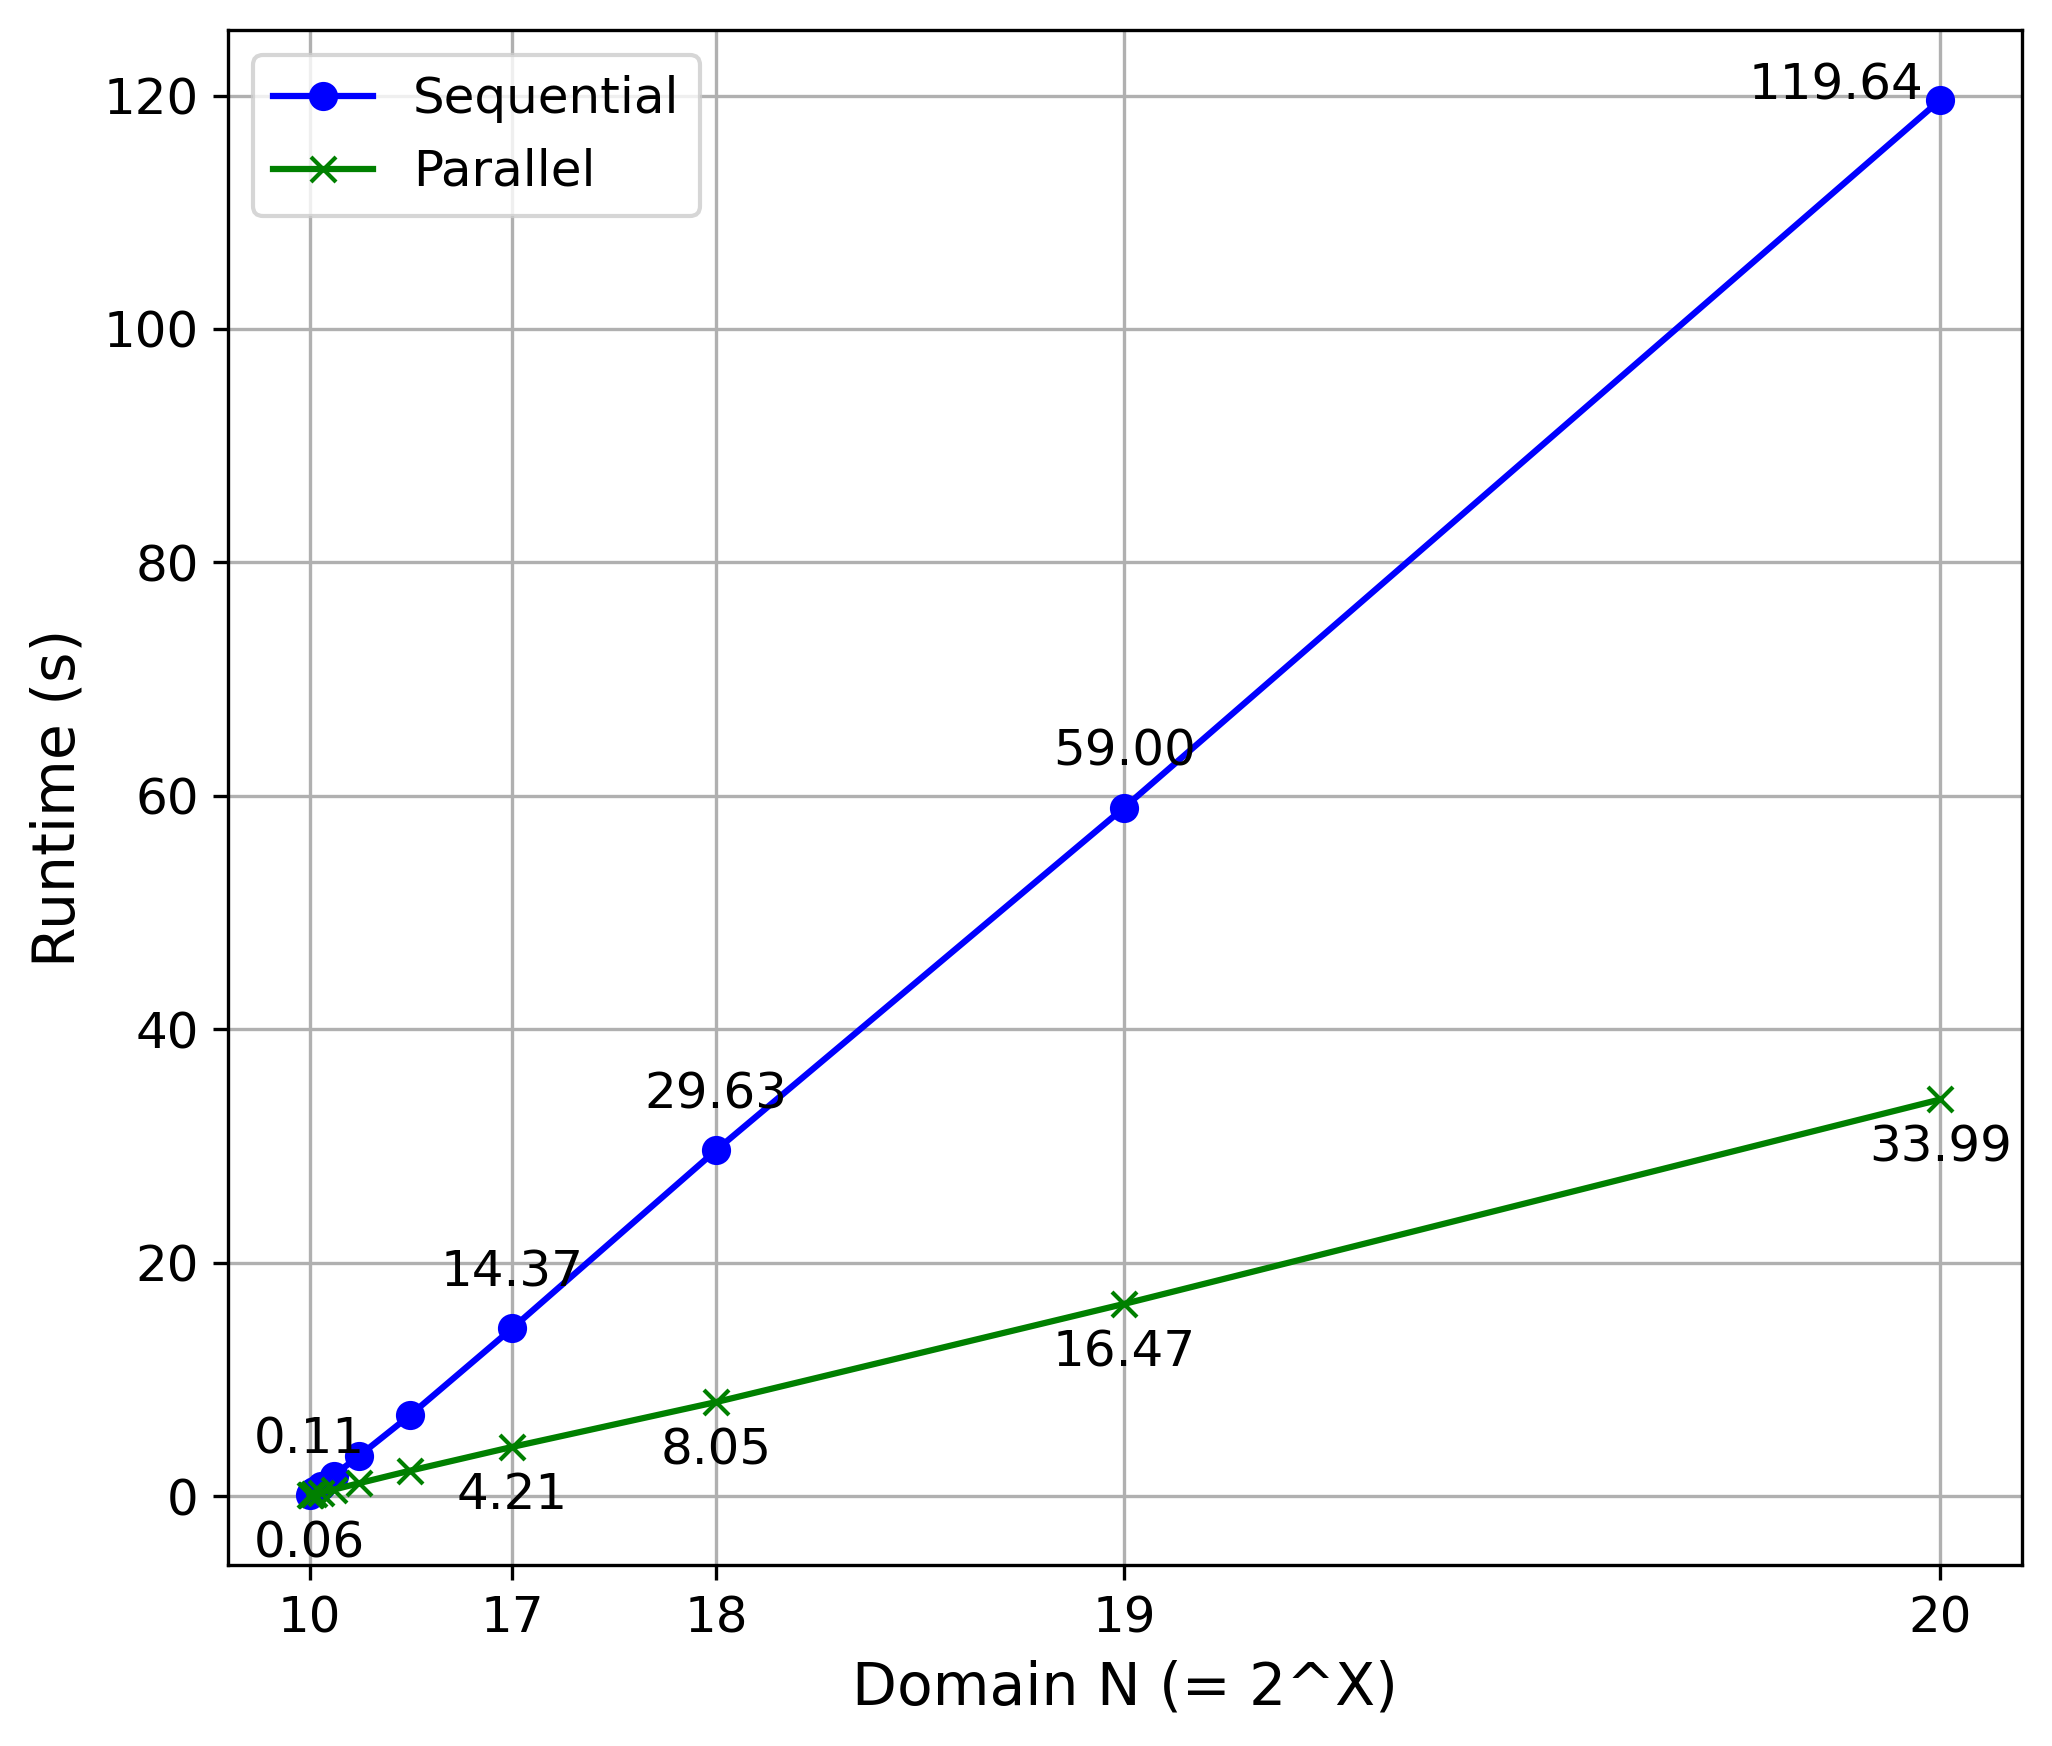
\includegraphics[scale=0.49]{images/plots/full_eval_t16.png}
        \caption{$p = \tau = 16$}
    \end{subfigure}
    \hspace{0em}
    \begin{subfigure}[b]{0.5\textwidth}
        \centering
        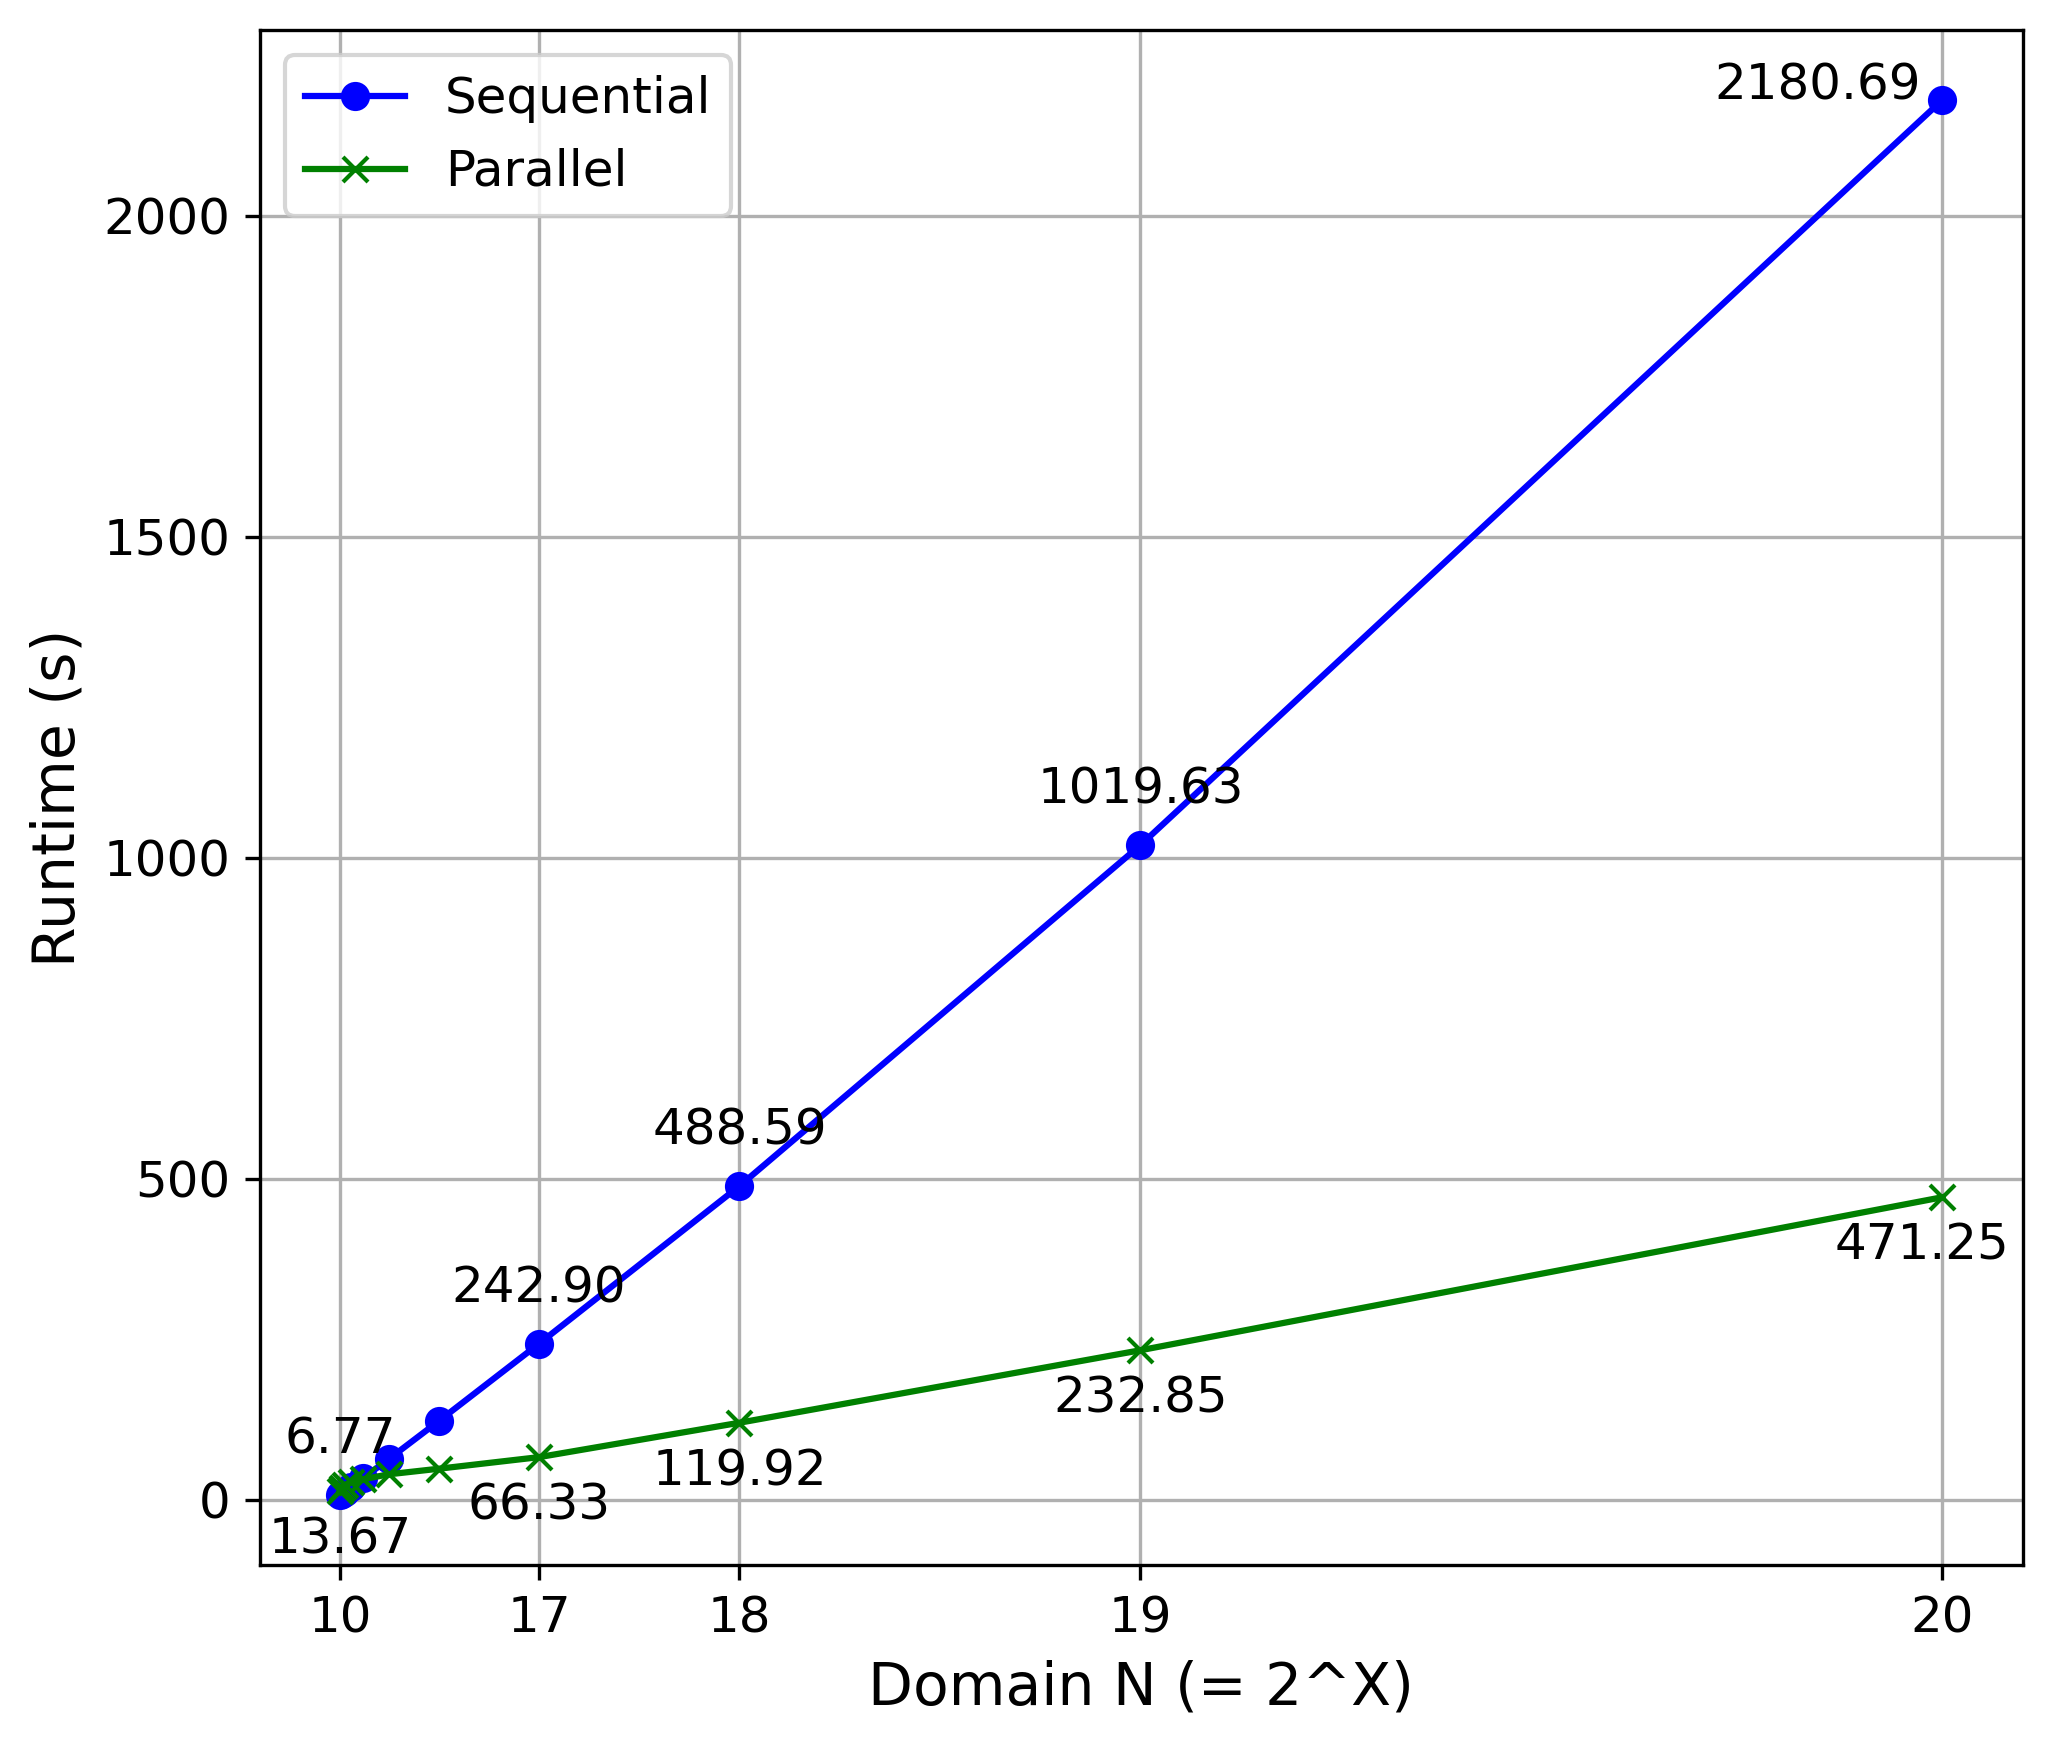
\includegraphics[scale=0.49]{images/plots/full_eval_t256.png}
        \caption{$p =\ tau^2 = 256$}
    \end{subfigure}
    \caption{Comparison of sequential and parallel processing of \texttt{DSPF.FullEval}$_N^p$ for $t=16$}
    \label{fig:fullEvalChart}
\end{figure}

\subsection{Operations on Polynomials of High Degree}
\label{subsec:evalOpOnHighDegreePoly}
In the following, we evaluate the runtime of our polynomial arithmetic implementation, specifically optimized for the PCG use case, where support for high-degree polynomial operations is needed. We evaluate the techniques proposed in Section \ref{sec:polyOperationsImpl} for polynomials of up to degree $2^{20}$. These include the Fast Fourier Transform (FFT), sparse polynomial multiplication, and Horner's method. The results indicate that the PCG construction benefits significantly from the strategic use of the techniques used. Without these optimizations, the PCG would not be practical within reasonable time constraints.

\subsubsection{Dense Multiplication}
Dense degree $N$ polynomials possess non-zero coefficients for all terms ranging from the constant to $x^N$. As detailed in Section \ref{subsec:multviaFFT}, their naive multiplication has a computational complexity of $O(N^2)$. On the contrary, the Fast Fourier Transform (FFT) optimizes this operation to $O(N \log N)$. In Figure \ref{fig:polyMultNaiveVsFFT} we present benchmarks for both approaches for $N\in \{2^{10}, ..., 2^{20}\}$. The results confirm the stark difference in scaling: The naive approach demonstrates significantly worse performance compared to the quasilinear runtime achieved by the FFT. The difference between both approaches underlines the importance of using FFT for high-degree polynomial multiplications and, therefore, the PCG implementation.

\begin{figure}[t]
    \centering
    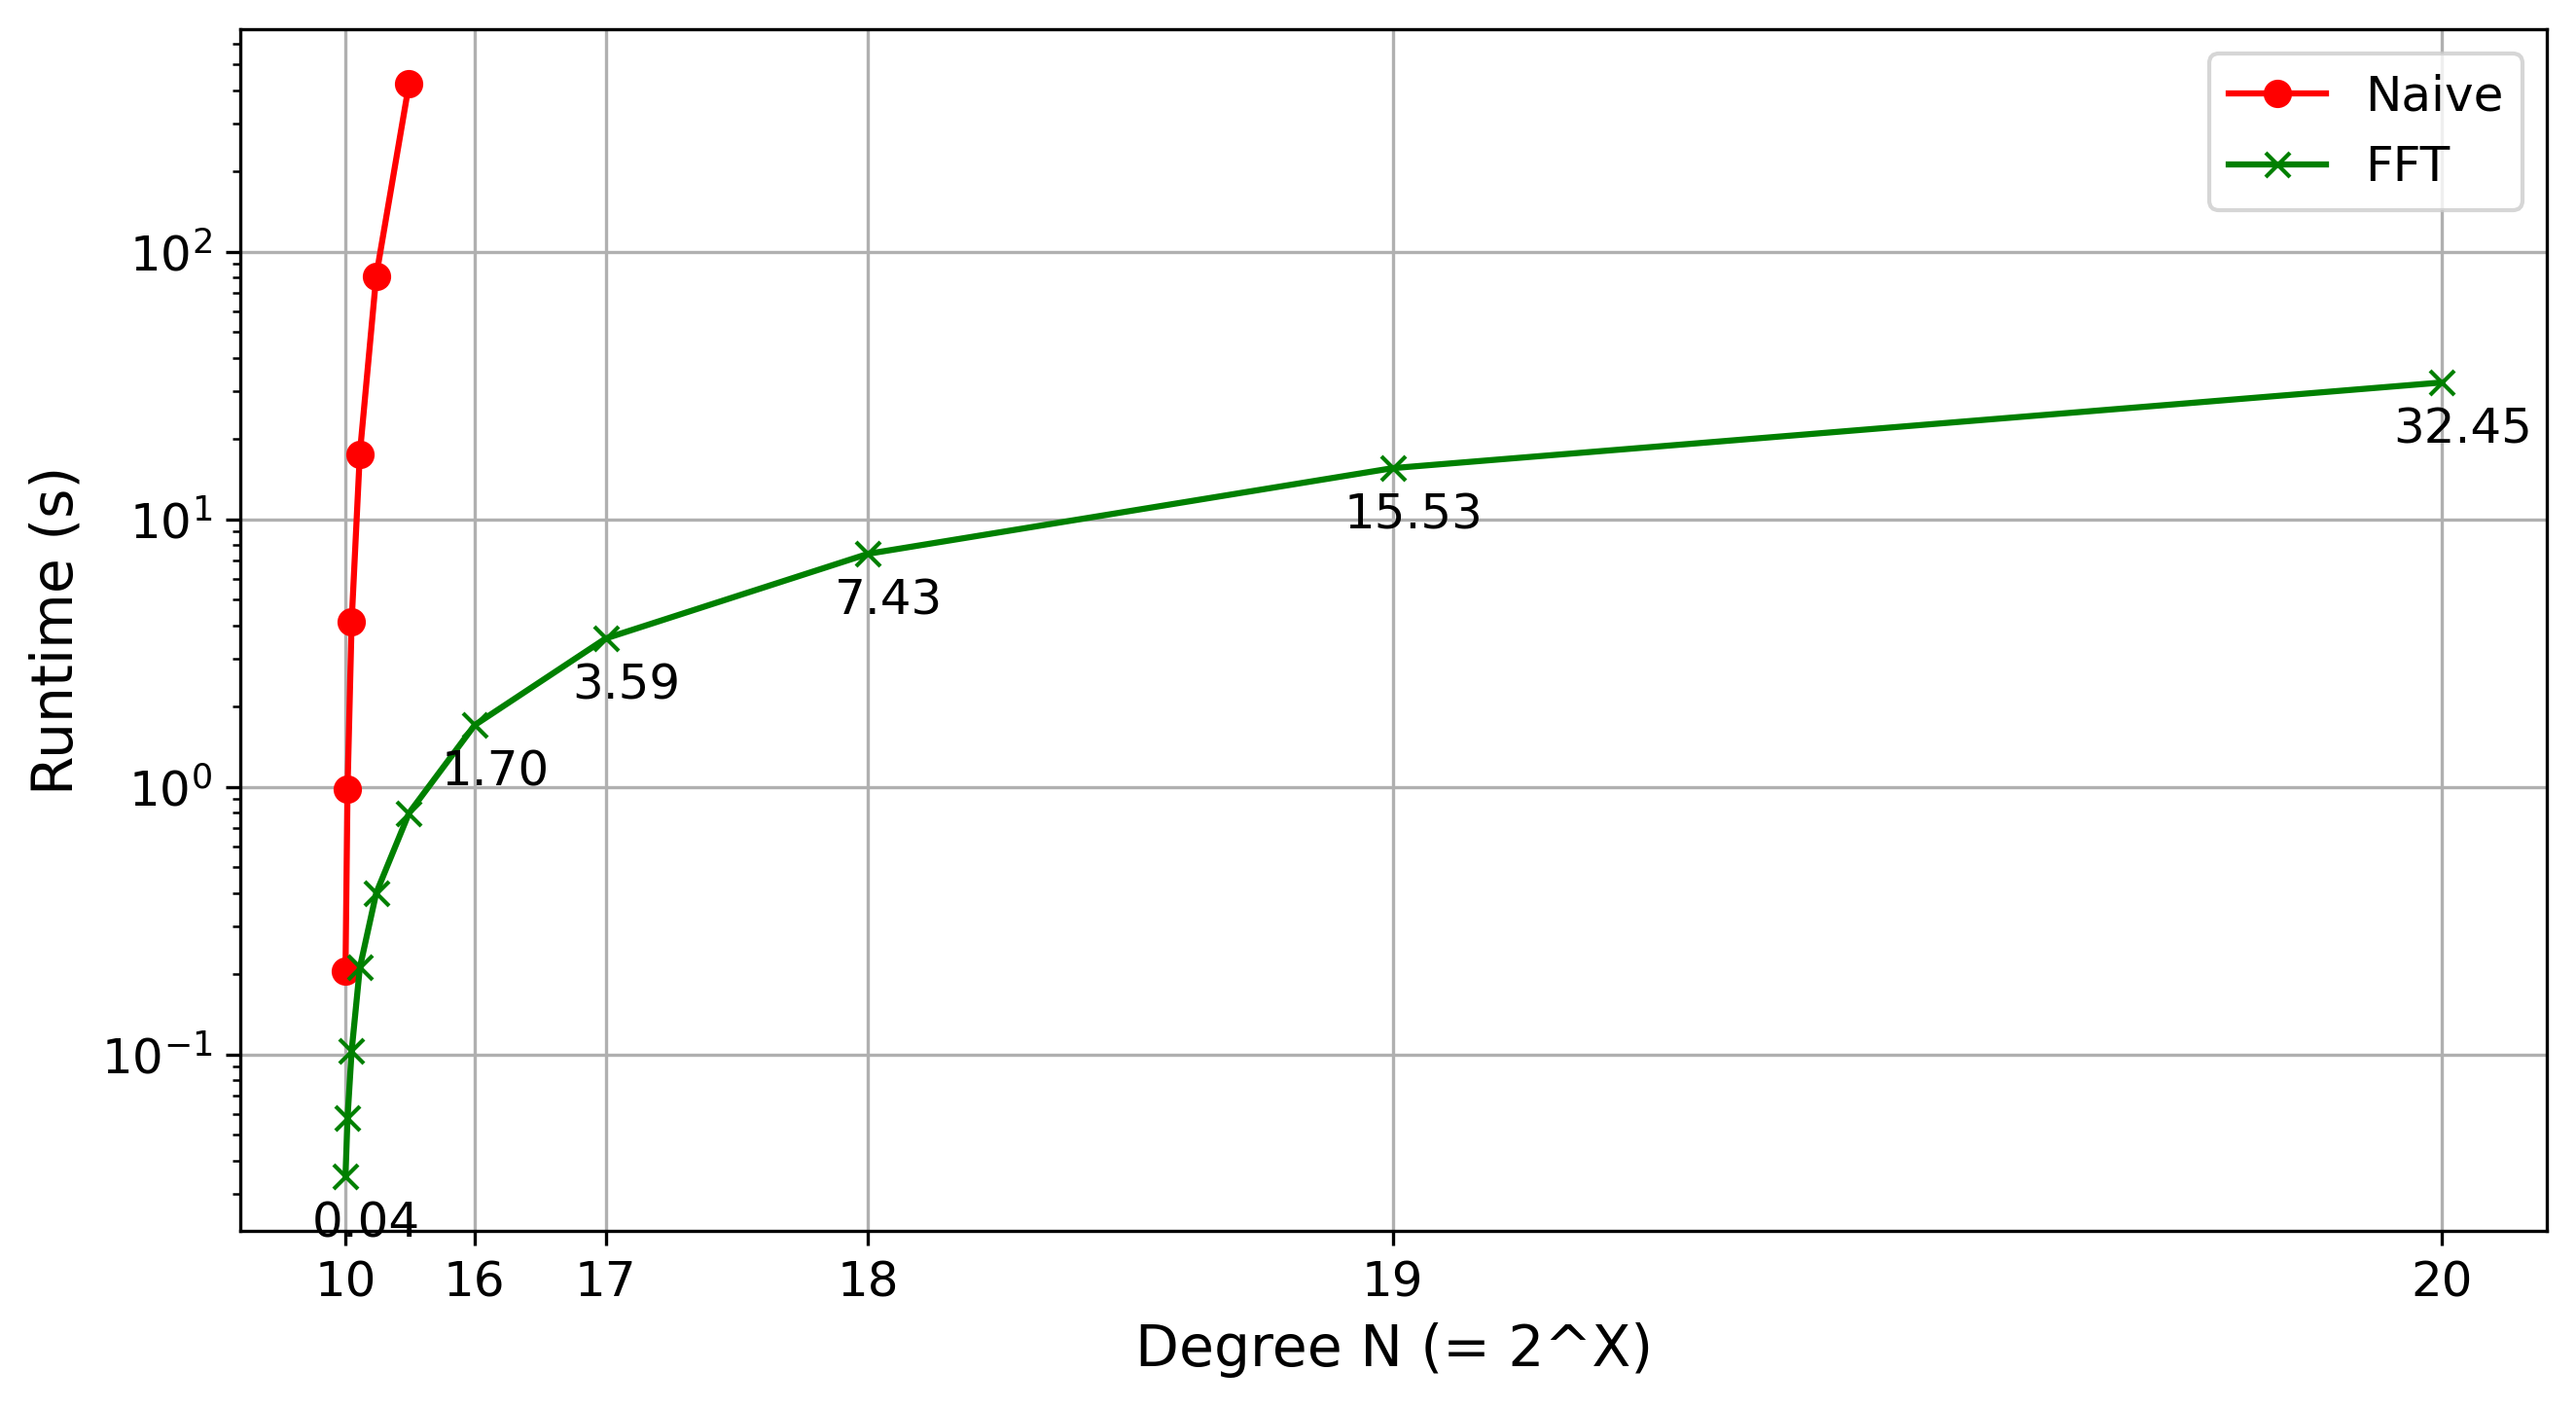
\includegraphics[scale=0.49]{images/plots/poly_mult.png}
    \caption{Comparing approaches to polynomial multiplication of two dense degree $N$ polynomials}
    \label{fig:polyMultNaiveVsFFT}
\end{figure}

\subsubsection{Sparse Multiplication}
Sparse polynomials of degree $N$ possess only a few non-zero coefficients within the terms ranging from the constant to $x^N$. In Section \ref{subesec:exploitingSparsity}, we claim that, for certain scenarios, naive multiplication of sparse polynomials could outperform the FFT when zero-coefficient multiplications are efficiently handled. Figure \ref{fig:naiveVsFFTSparsePolys} validates this claim by benchmarking the multiplication of polynomials with varying sparsity for degrees $N=2^{15}$ and $N=2^{18}$. As the complexity of FFT depends solely on the degree of the result, its runtime remains constant for a fixed $N$.  Conversely, the naive approach scales quadratically with sparsity but exhibits significantly lower runtimes for very sparse polynomials. Importantly, the higher the degree $N$, the wider the sparsity range where the naive approach outperforms FFT. In practice, accounting for this in the PCG implementation poses a significant performance increase as the LPN error polynomials are chosen $\tau$-sparse. When we account for $\tau=16$ and $N=2^{18}$, a naive multiplication takes only a few ms instead multiple seconds using FFT.

\begin{figure}[t]
    %\centering
    \hspace{-1em}
    \begin{subfigure}[b]{0.5\textwidth}
        \centering
        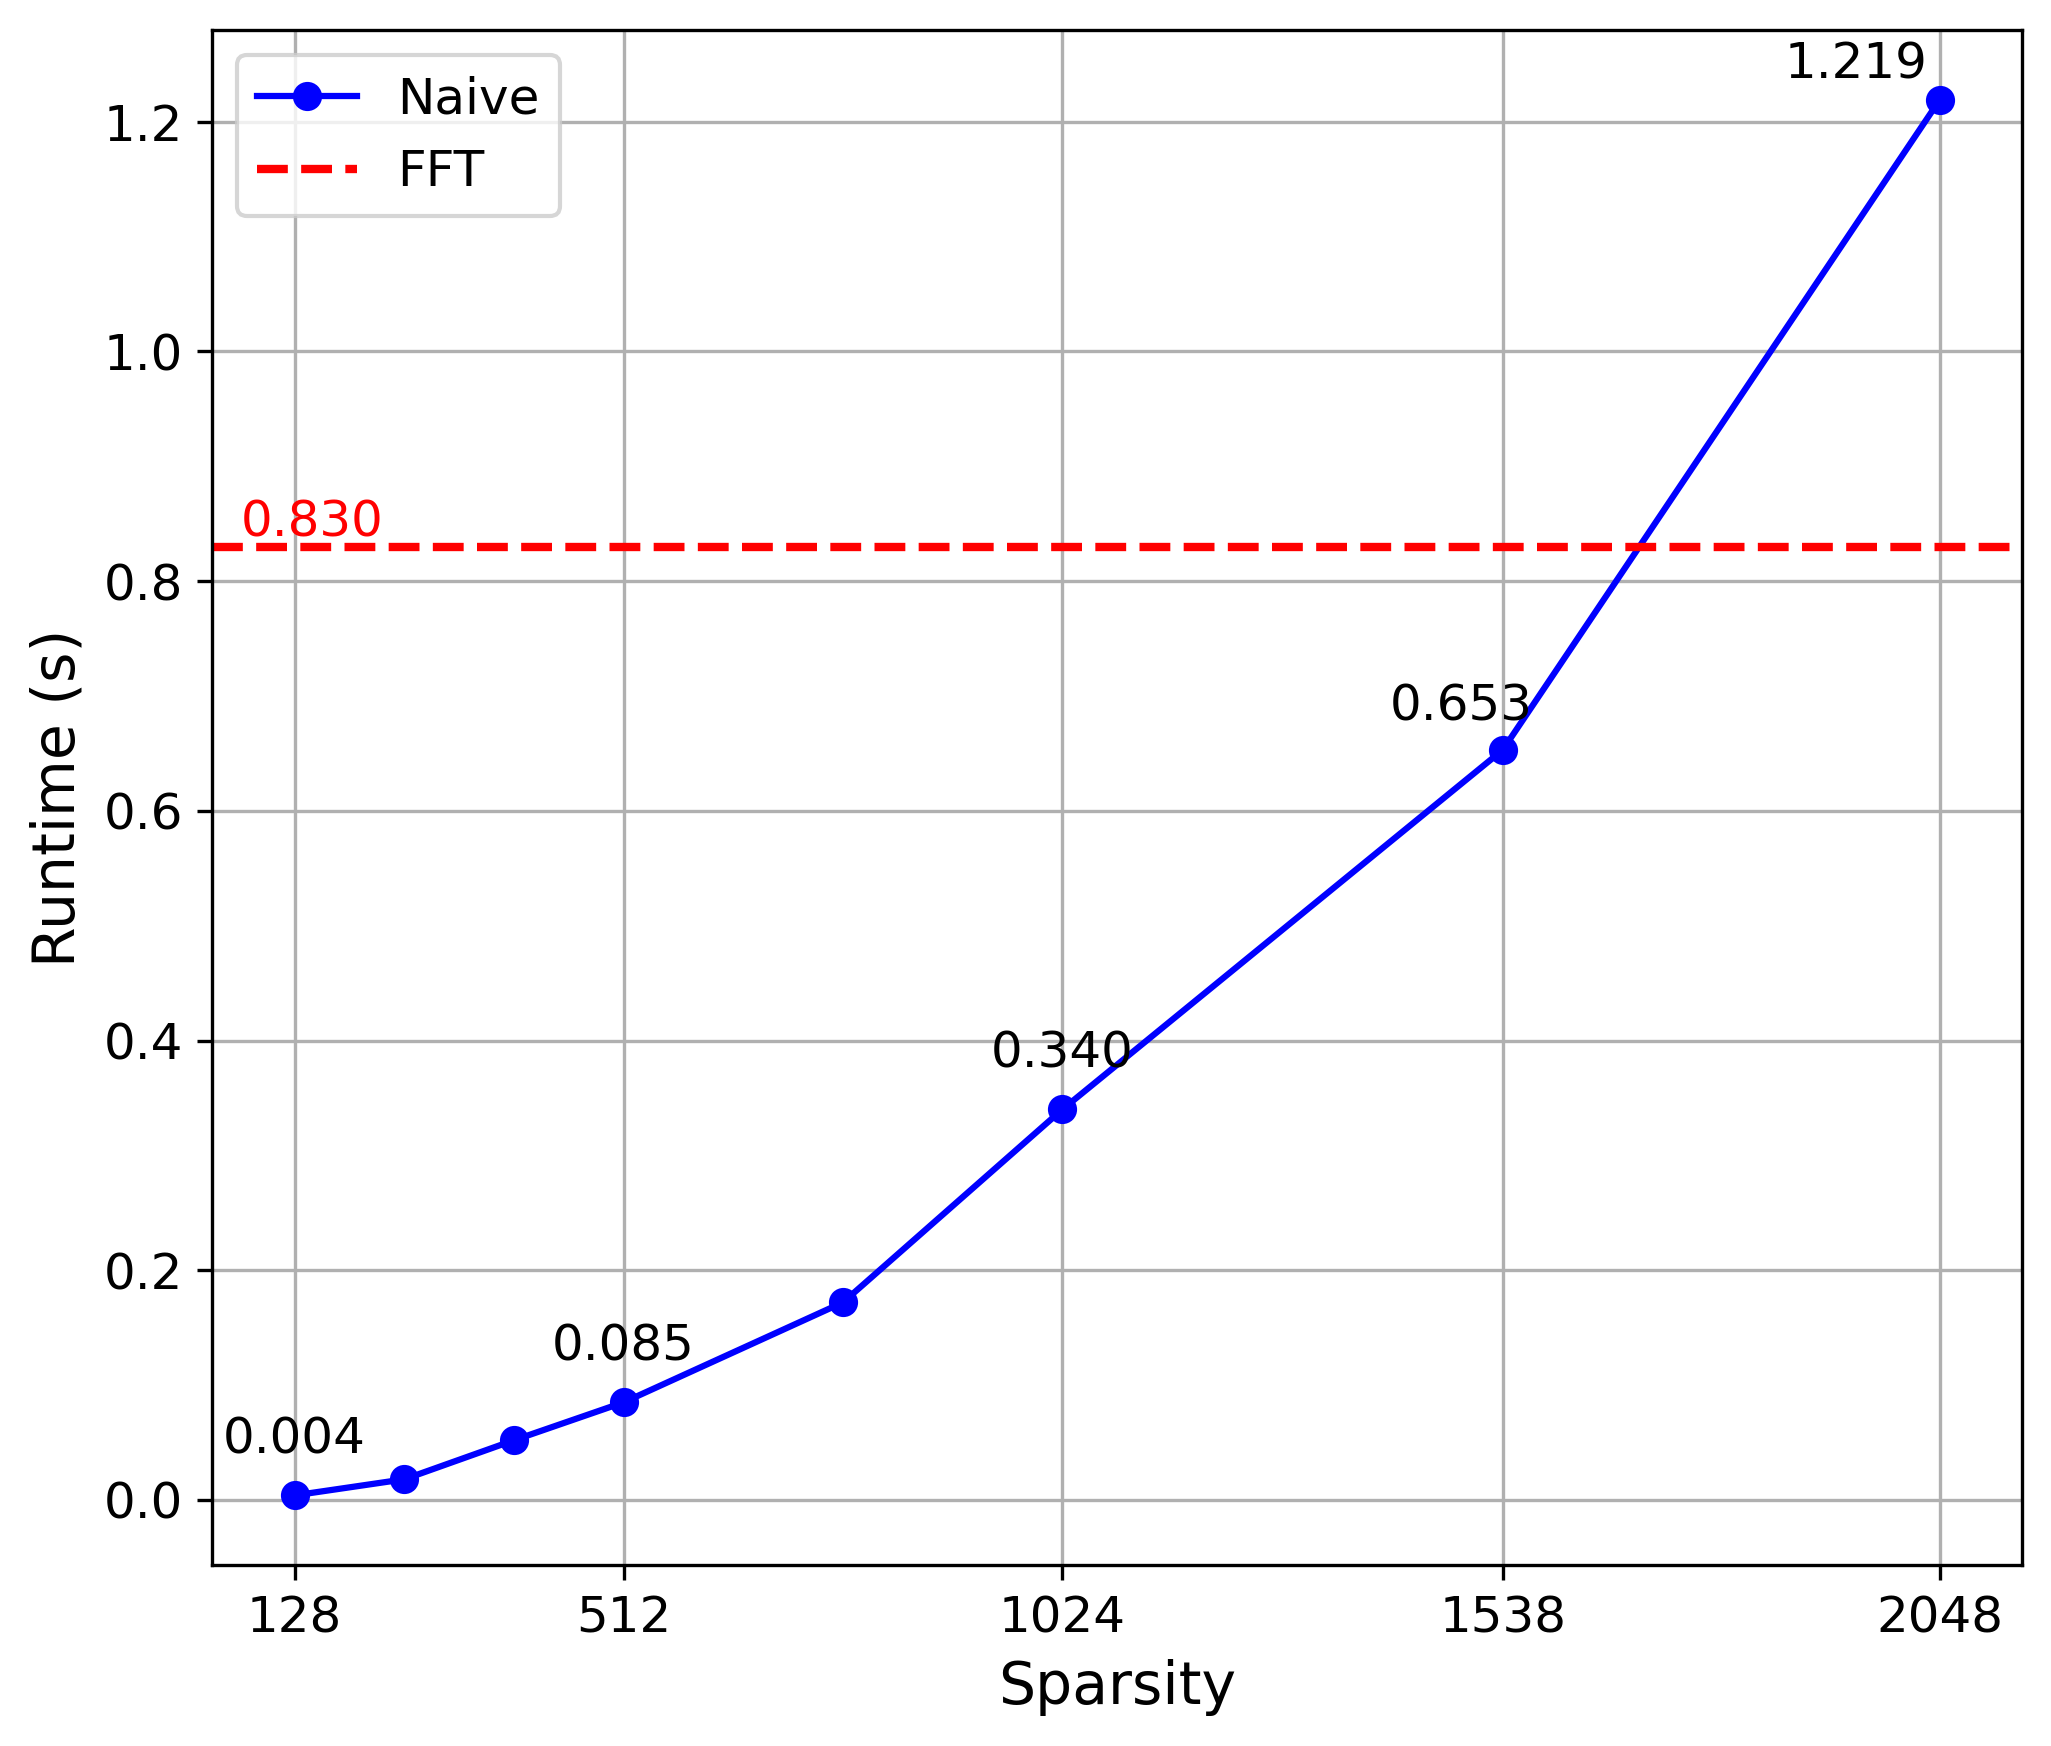
\includegraphics[scale=0.49]{images/plots/poly_mult_sparse_N15.png}
        \caption{$N=2^{15}$}
    \end{subfigure}
    \hspace{0em}
    \begin{subfigure}[b]{0.5\textwidth}
        \centering
        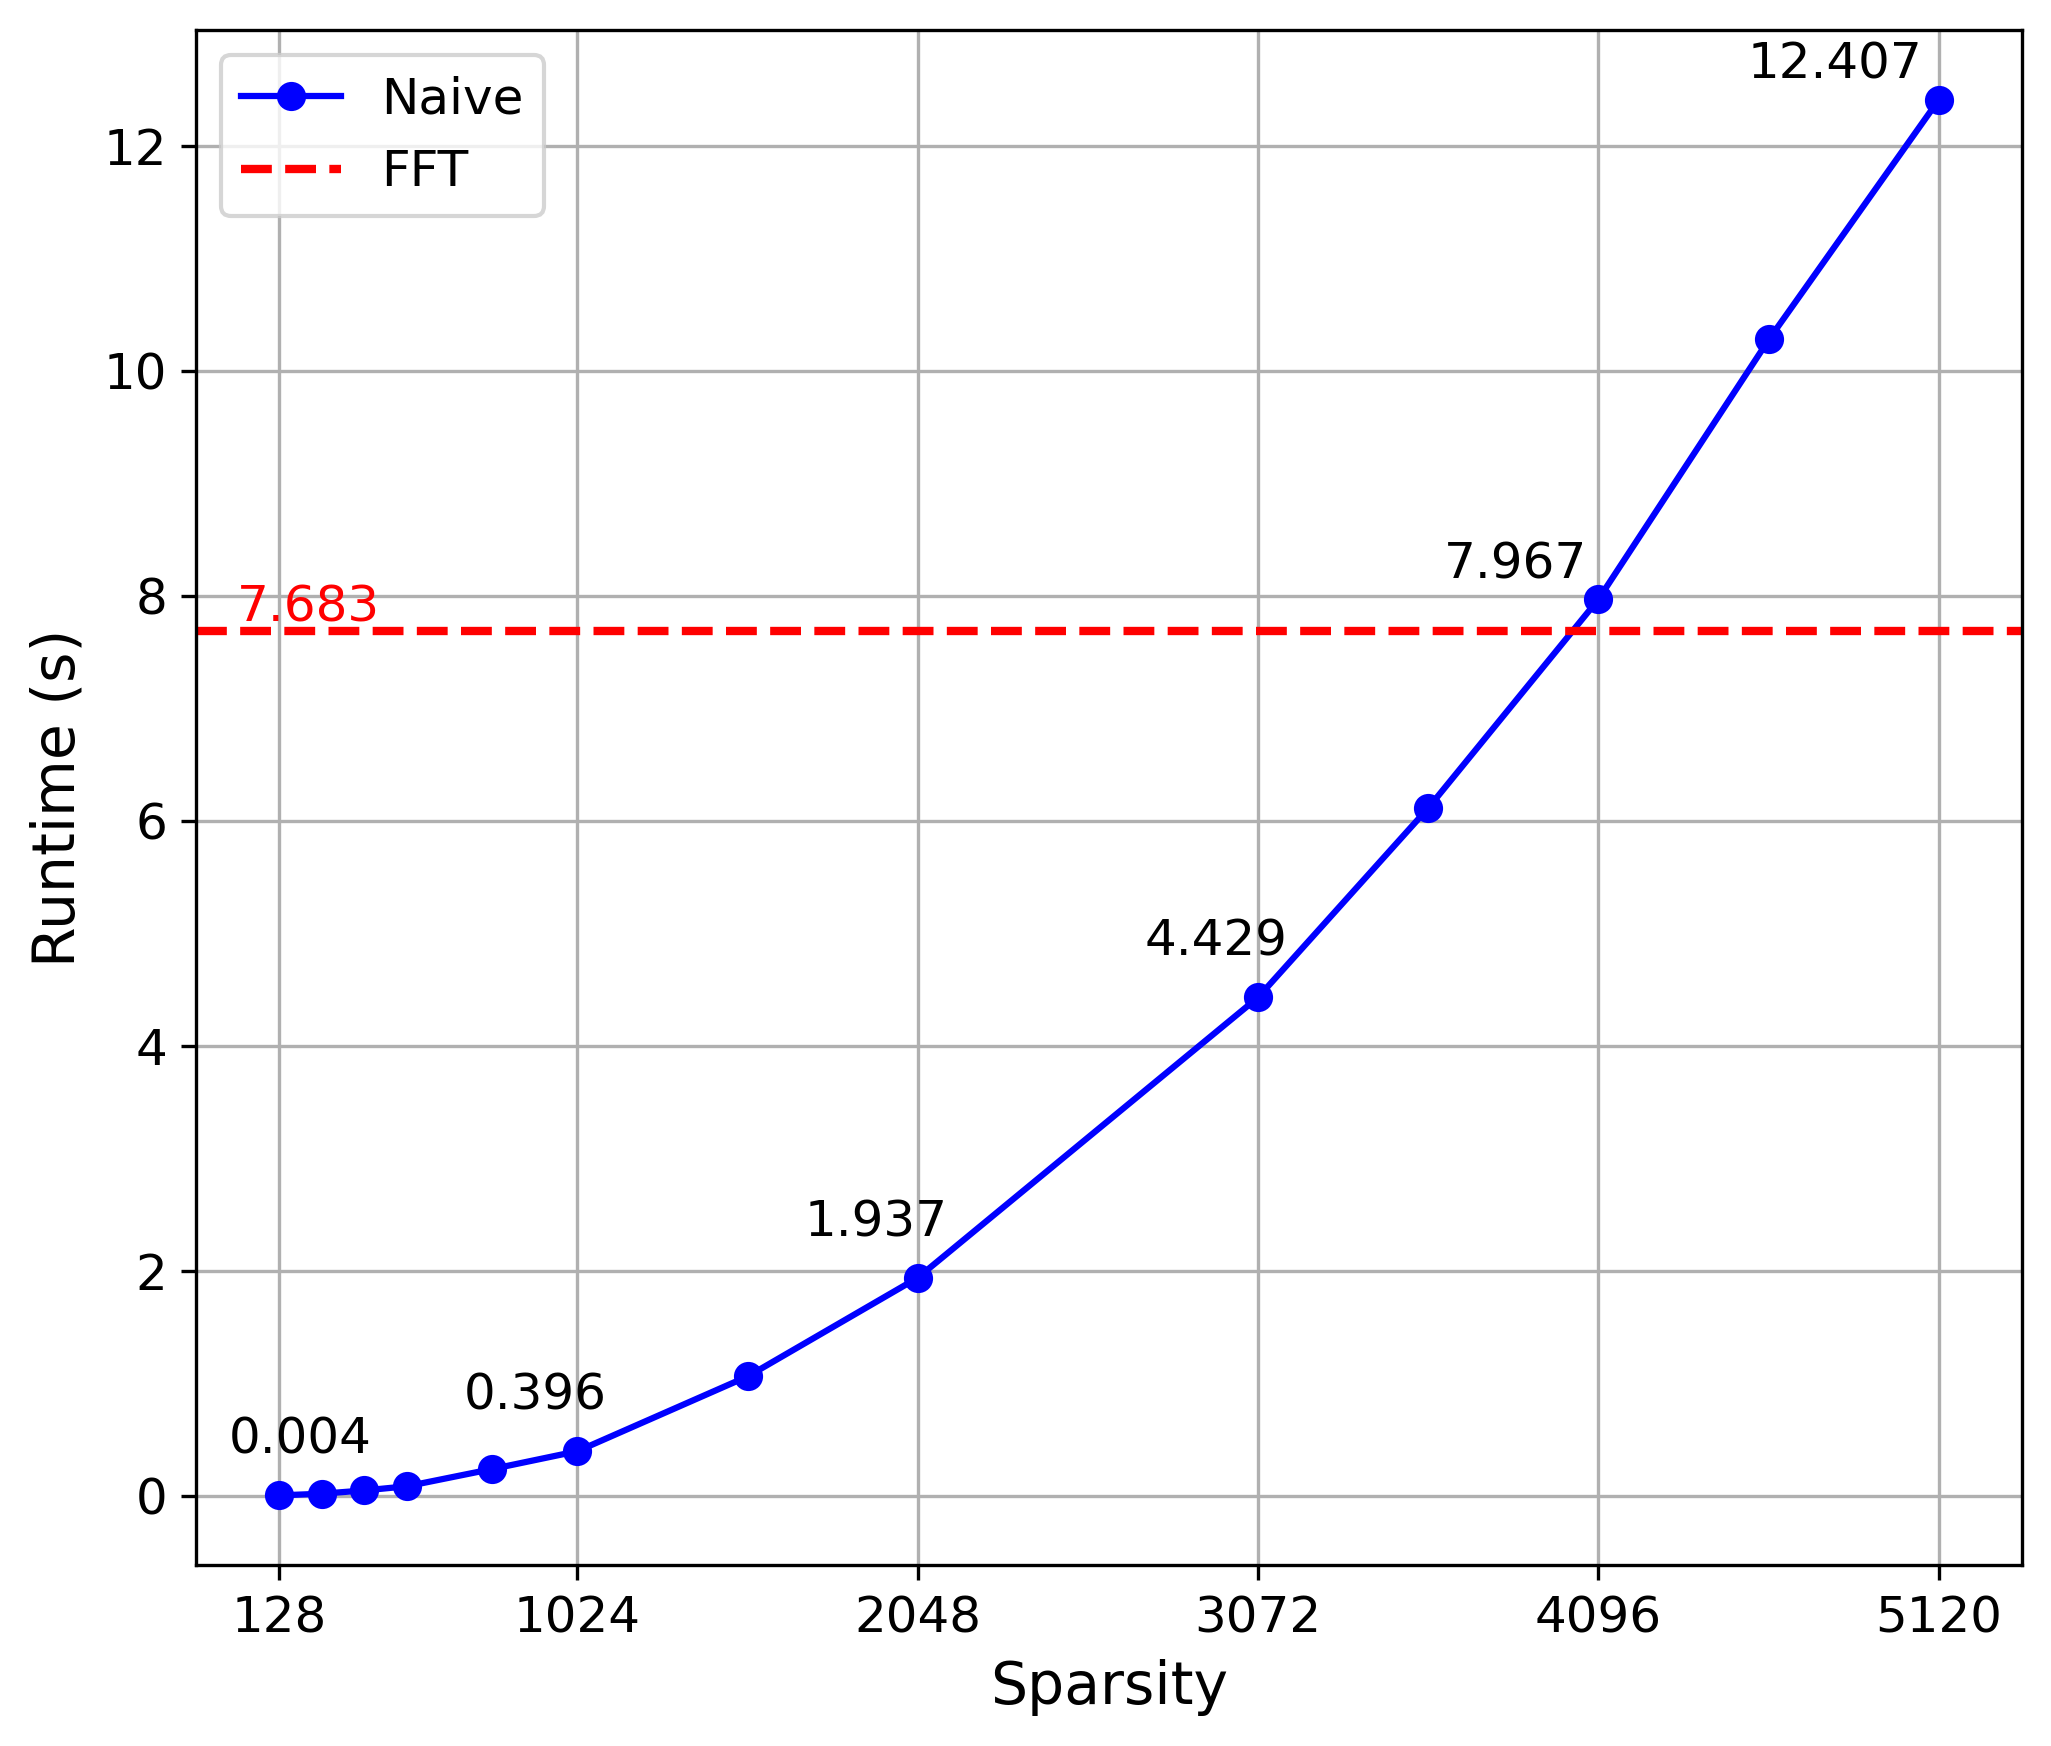
\includegraphics[scale=0.49]{images/plots/poly_mult_sparse_N18.png}
        \caption{$N=2^{18}$}
    \end{subfigure}
    \caption{Comparing approaches to polynomial multiplication of two sparse degree $N$ polynomials}
    \label{fig:naiveVsFFTSparsePolys}
\end{figure}

\subsubsection{Evaluation}
In Section \ref{subsec:horner}, we outline how Horner's method optimizes polynomial evaluation to achieve linear $O(N)$ complexity, a significant improvement over the naive quadratic approach. To validate this, we present benchmarks for evaluating polynomials of degree $N \in \{2^{11}, ..., 2^{20}\}$ in Figure \ref{fig:polyEvalBench}. As expected, the naive approach shows worse performance, especially as $N$ increases. Horner's method demonstrates a clear linear runtime increase, enabling the evaluation of a degree $N=2^{20}$ polynomial at a specific position in approximately 165ms. However, after PCG expansion, $N$ individual position needs to be evaluated on (multiple) polynomials to extract all (V)OLE correlations. This underscores the importance of polynomial evaluation for the PCG.
\\\\
\textbf{Parallelization.} To address a potential bottleneck, we explore parallelization. Unlike parallelizing multiple evaluations, our strategy directly enhances performance for single-point evaluations – potentially beneficial if storage complexity is a concern and parties split the ring on demand (cf. Section \ref{sec:fxconsiderationsImpl}). Our parallelized implementation of Horner's method achieves a near-10x speedup, demonstrating good hardware utilization. This reduces the evaluation time for a degree $N=2^{20}$ polynomial to 17.7ms, down from 165ms.

\begin{figure}[t]
    \centering
    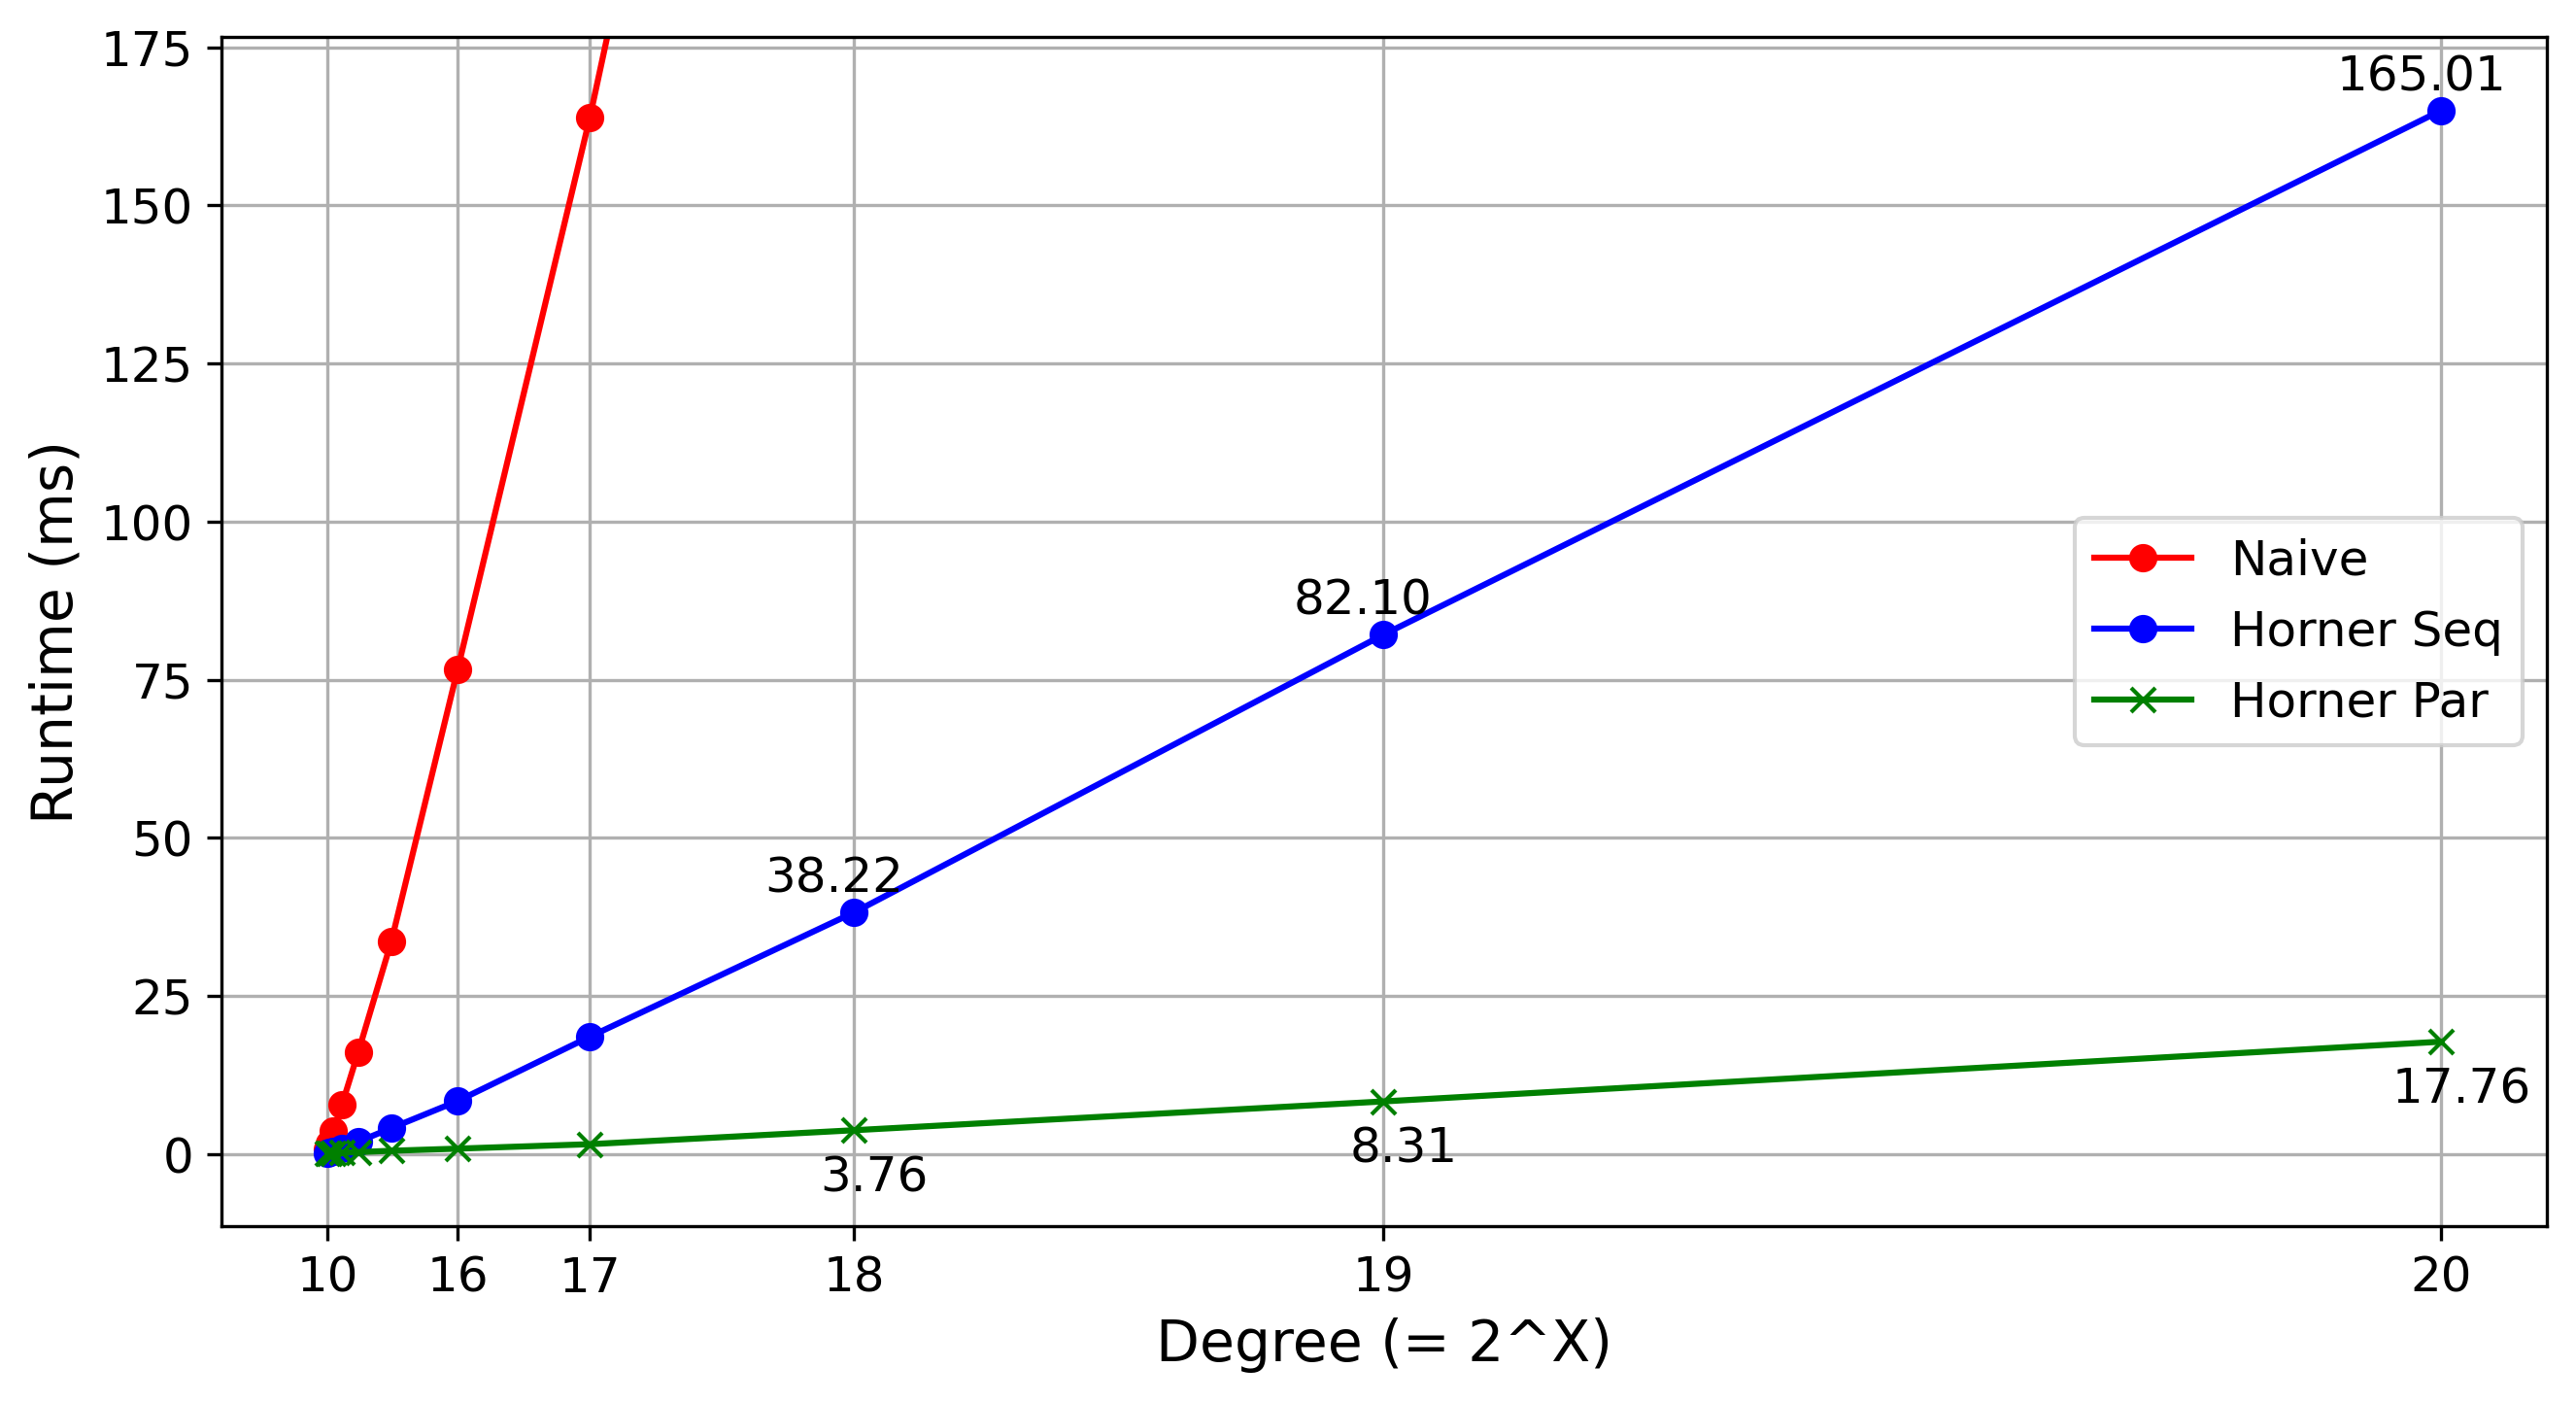
\includegraphics[scale=0.49]{images/plots/poly_eval.png}
    \caption{Comparing approaches to polynomial evaluation of a dense degree-$N$ polynomial}
    \label{fig:polyEvalBench}
\end{figure}


\subsection{Computing Roots of Unity}
\label{subsec:evalRootOfUnity}
In the following, we evaluate our implementation for computing all roots of unity for the $2N$-th cyclotomic polynomial. As outlined in Section \ref{sec:fxconsiderationsImpl}, we implemented two approaches: the naive method directly iterates over Equation \ref{eq:root_main_equasion} to generate all roots of unity, while the optimized approach leverages a Horner inspired technique to reuse exponentiations for improved efficiency. The benchmarks for $N=\{2^{15}, ..., 2^{20}\}$ (Figure \ref{fig:ComparingRootOfUnityAp}) show that the optimized approach scales linearly. This is beneficial for PCG construction, as it does not negatively affect the time required per (V)OLE correlation for higher PCG domains. Note also that we achieve a significant performance improvement of about 11x over the naive method.

\begin{figure}[t]
    \centering
    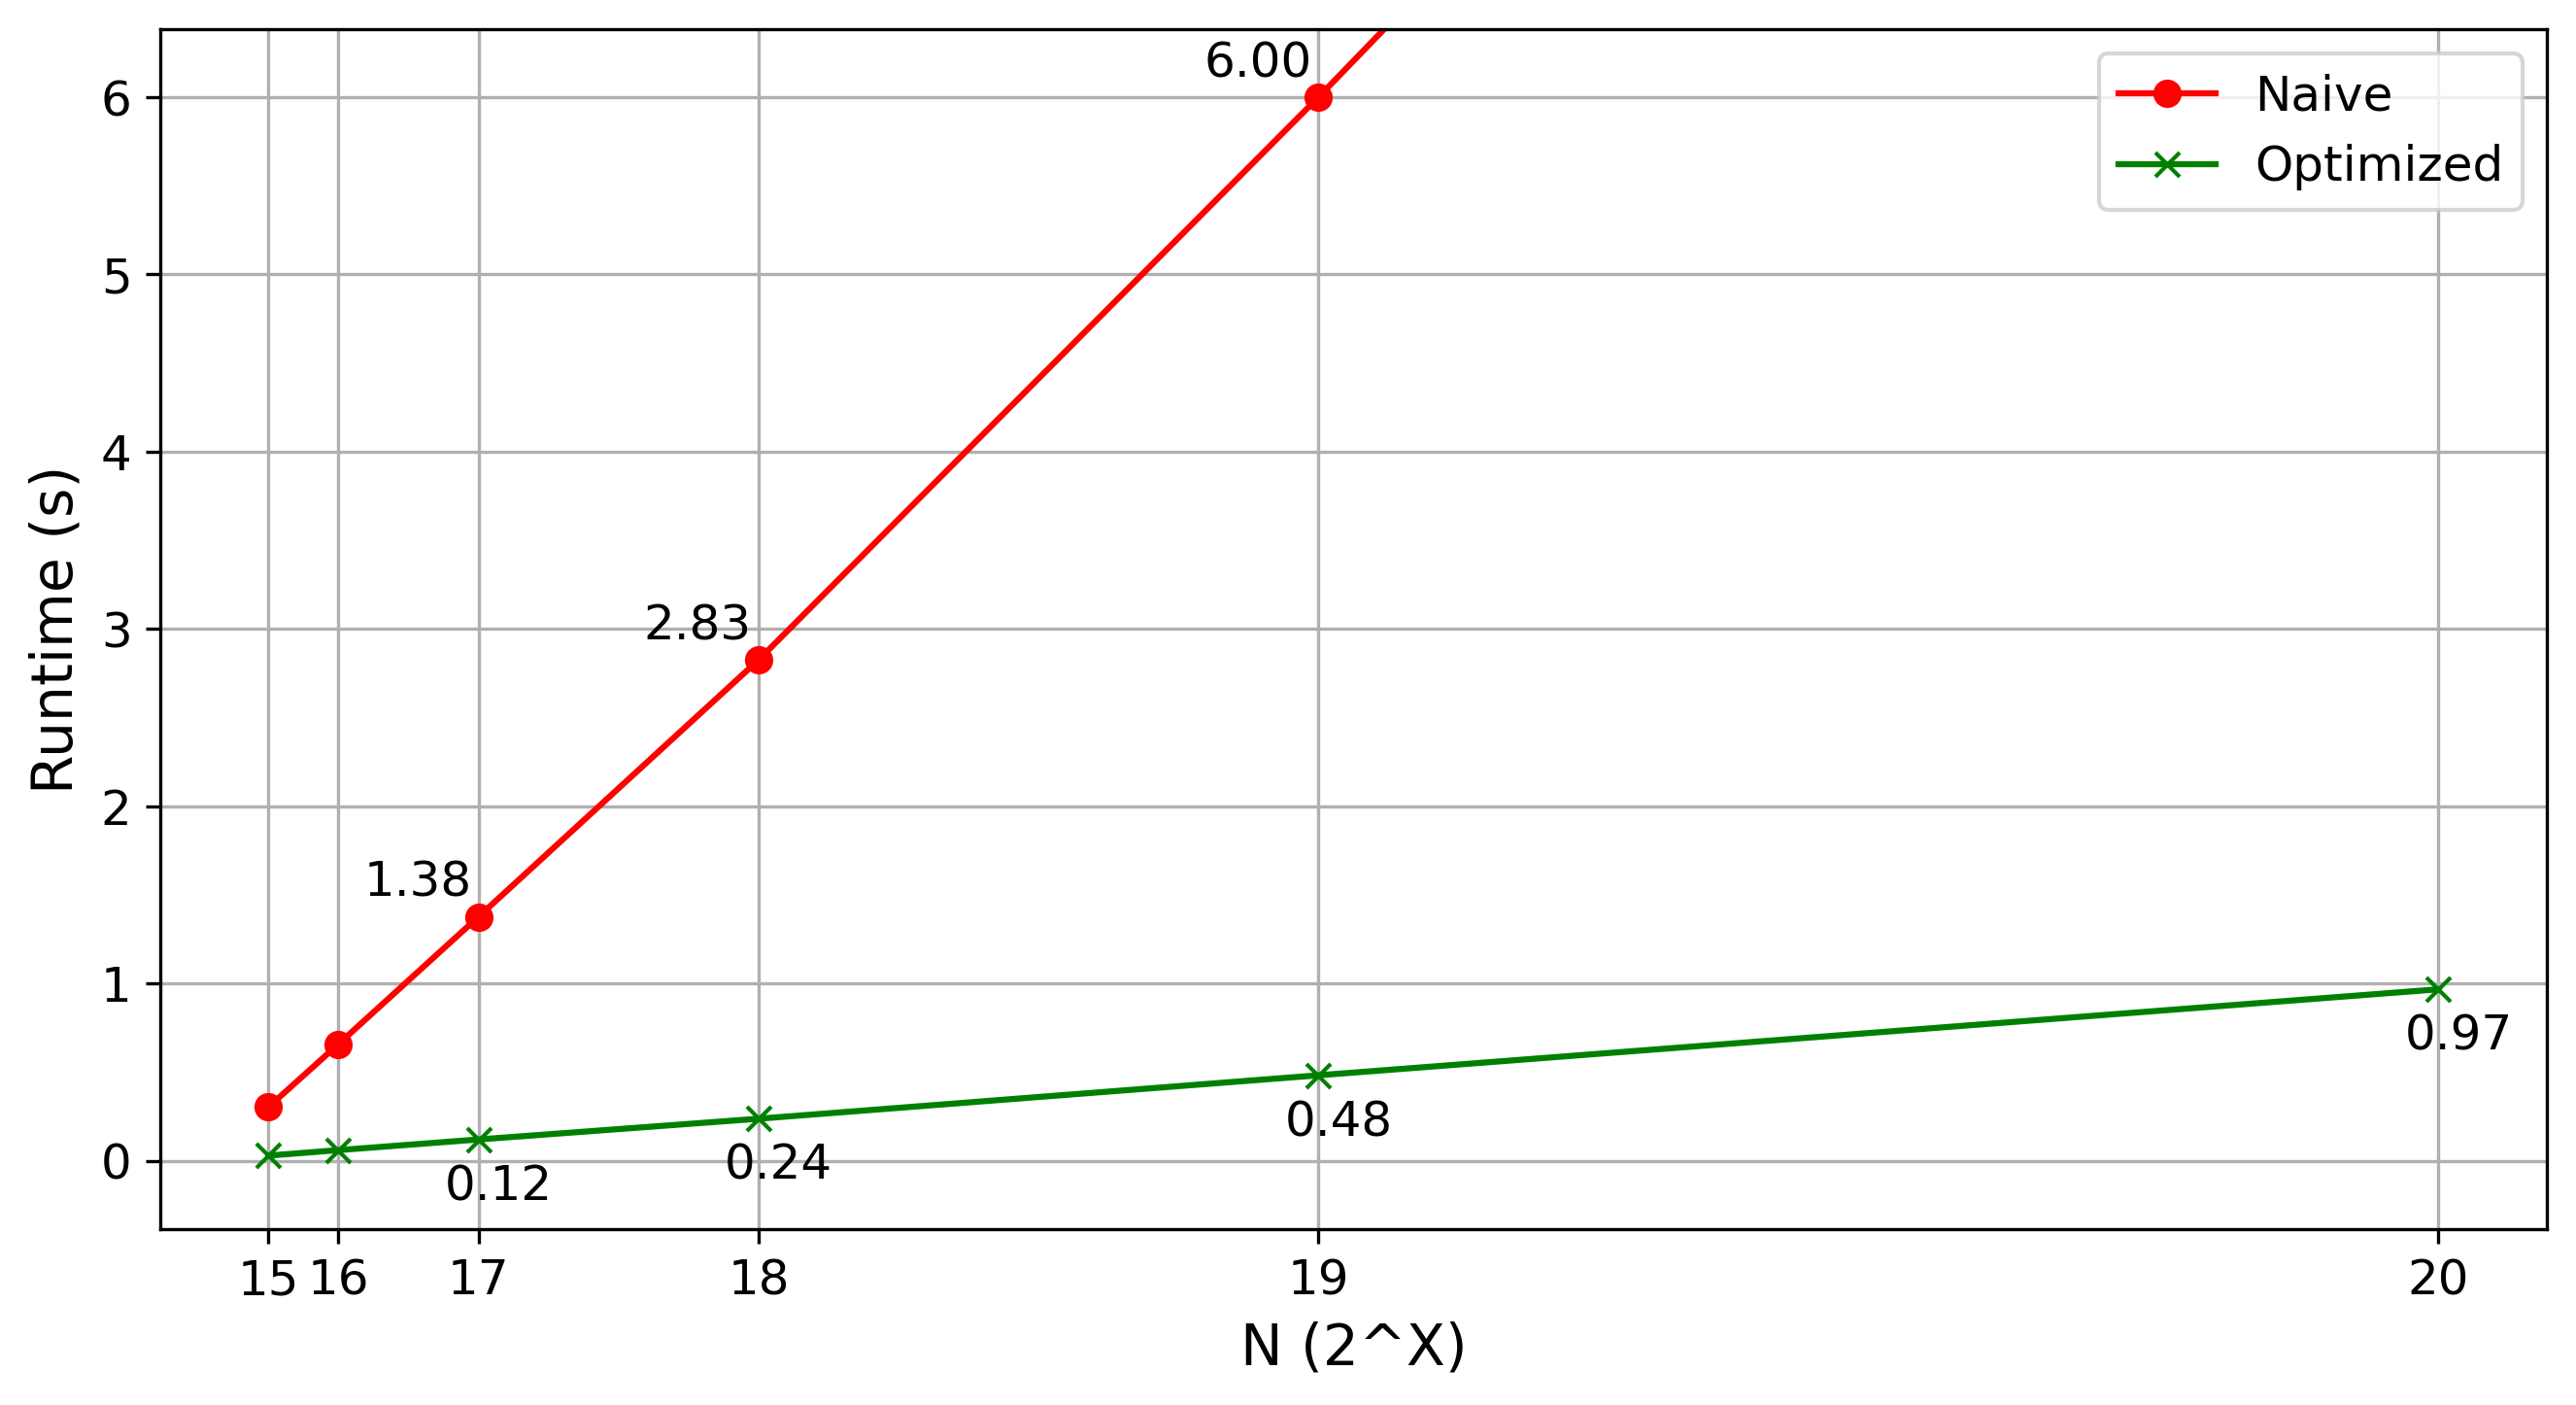
\includegraphics[scale=0.49]{images/plots/gen_roots.png}
    \caption{Comparing approaches to generate all \textit{roots of unity} for the $2N$-th cyclotomic polynomial}
    \label{fig:ComparingRootOfUnityAp}
\end{figure}


\section{PCG Construction}
In this section, we evaluate the PCG construction presented in Section \ref{subsec:VOLEConstruction} for different domains $N$. We choose the LPN parameters to be $(c,\tau)=(4,16)$ which achieve $128$-bit security, as reported by Boyle et al. \cite{boyle2020efficient}. 
% Benchmarks are conducted for domain sizes $N\in\{2^{10}, ..., 2^{18}\}$. 

\subsection{Generation}
\label{subsec:evalGen}
Figure \ref{fig:ComparingPCGGeneration} presents the runtime of PCG seed generation, particularly when using a trusted dealer. This contrasts with the higher overhead of distributed generation algorithms, which are not part of this work. It is worth noting that distributed generation alternatives exist, but they introduce significant performance tradeoffs.
\\\\
The VOLE construction requires four calls to \texttt{DSPF$^{t}_{N}$.Gen}. With $t=16$, this translates into 64 underlying DPF calculations (cf. Section \ref{subseq:constructingTBDSPFs}). On the contrary, the OLE construction performs 16 calls to \texttt{DSPF$^{\tau^2}_{2N}$.Gen}, demanding a significantly higher 4096 DPF computations. This 64x increase in DPFs aligns well with the benchmark results. For $N=2^{18}$, the OLE runtime of 0.44s is approximately 68 times longer than the VOLE's 0.0064s. Interestingly, the domain size $N$ has a relatively minor impact on generation time. This comes from the tree-based approach used within the underlying DPFs. Doubling $N$ leads to a roughly constant increase in operations (proportional to $\tau$ or $\tau^2$), due to the fixed value of $\tau$. 

\begin{figure}[t]
    \centering
    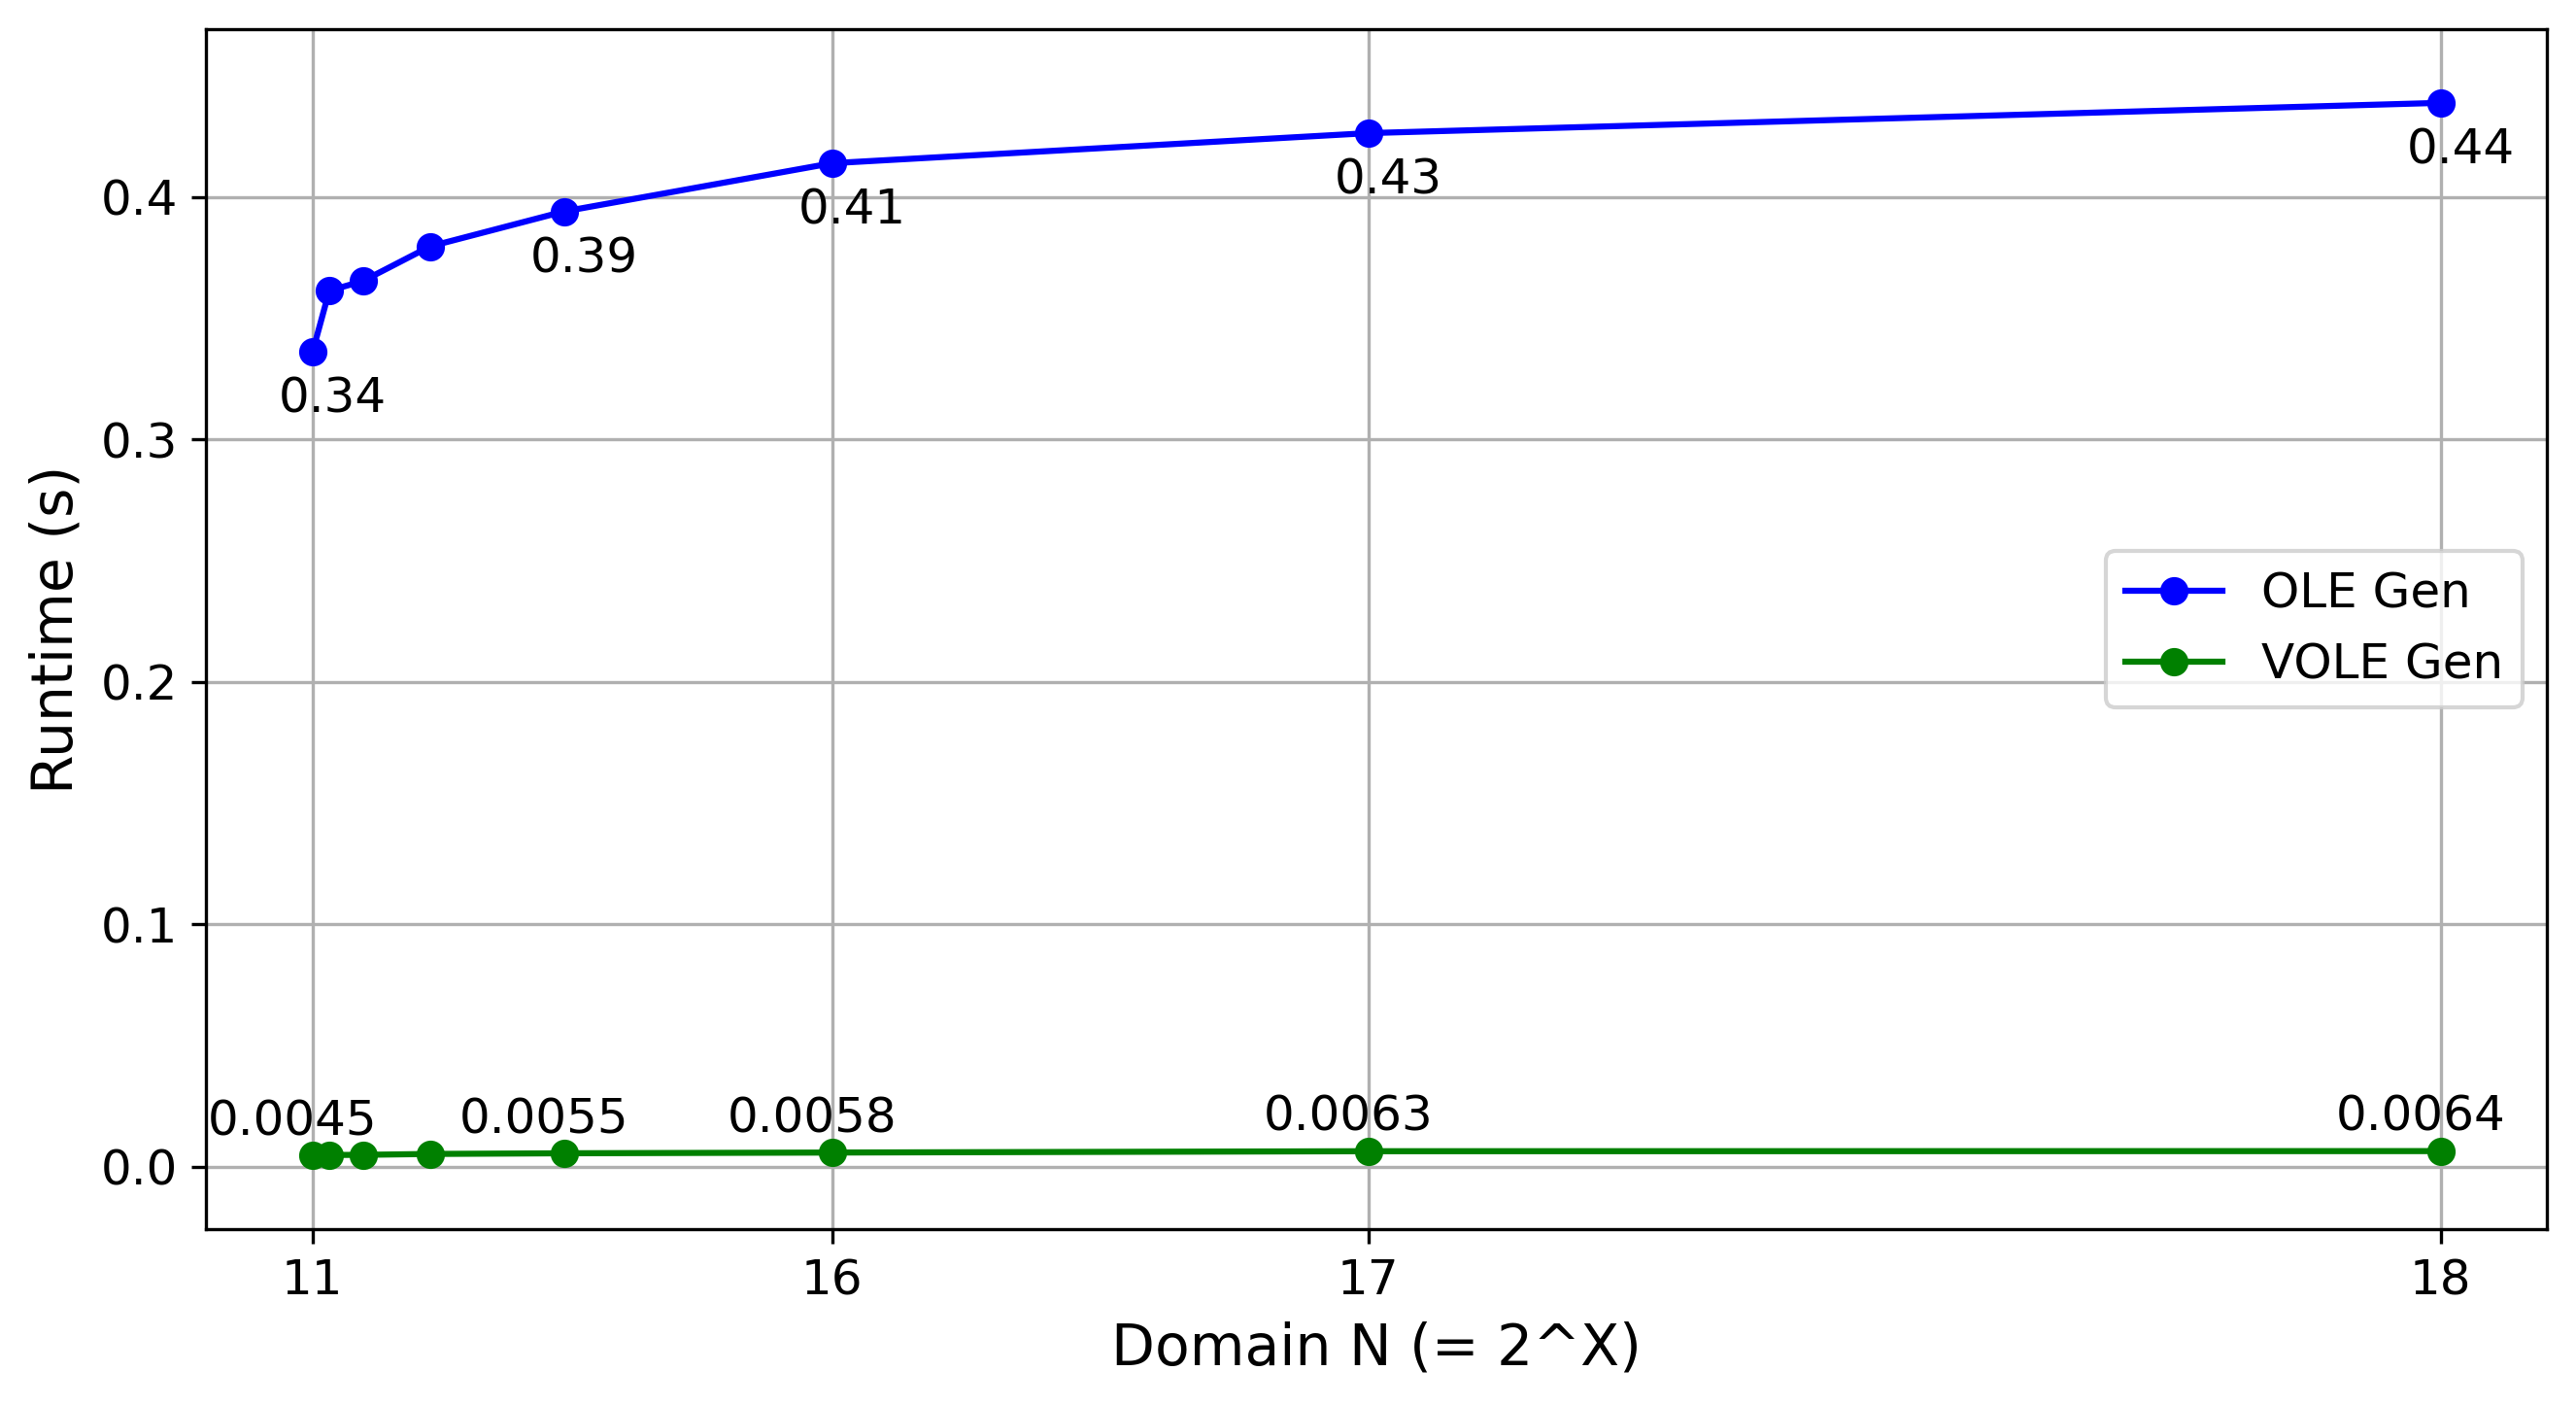
\includegraphics[scale=0.49]{images/plots/pcg_gen.png}
    \caption{Comparing the PCG expansion OLE and VOLE}
    \label{fig:ComparingPCGGeneration}
\end{figure}

\subsection{Expansion}
\label{subsec:evalExpansionVOLE}
We present the runtimes of the PCG constructions relative to the amount of (V)OLE correlation they generate in Figure \ref{fig:ComparingPCGExpansion}. This figure also separately visualizes the added cost of extracting correlations (splitting the ring elements) via polynomial evaluation on a root of unity. Observe the quasilinear scaling for both OLE and VOLE constructions with respect to $N$. As discussed previously, this primarily stems from the quasilinear nature of polynomial multiplication using FFT, despite achieving linearity in other building blocks. It is worth emphasizing that compared to the expansion itself, our optimized computation of roots of unity adds negligible overhead. For example, with $N=2^{18}$, this step adds only 0.24 ms per correlation. Therefore, this is not part of our evaluation.
\\\\
We observe a nearly exponential runtime increase in OLE construction for small $N$, transitioning to the expected quasilinear increase as $N$ grows. We identify this behavior as an effect of the parallelization overhead that dominates in small domains. As $N$ increases, the parallelization setup cost amortizes, revealing the construction's expected quasilinear runtime. The same applies to the VOLE construction, but is less visible due to the figures scaling. Notably, the VOLE construction scales more favorably than OLE construction, exhibiting a near-linear runtime. Several factors explain this:

\begin{itemize}
    \item \textbf{Reduced Multiplications:} With $c=4$, the VOLE construction requires only $8$ polynomial multiplications compared to OLE's $24$. Since multiplications (via FFT) drive the quasilinear runtime, their reduced usage in the VOLE construction yields a runtime closer to the complexity of other primitives.
    
    \item \textbf{Lower Degrees:} The multiplications of the VOLE construction operate on degree-$N$ polynomials, while a significant portion of OLE constructions multiplications involve degree-$2N$ polynomials. As FFT complexity becomes closer to linear for smaller degrees, this further reduces its overall impact in the VOLE construction.
    
    \item \textbf{Exploiting Sparsity:} The VOLE construction involves more sparse polynomial multiplications. Here, our optimized approach strategically selects the more efficient naive method, further improving performance.
\end{itemize}

\begin{figure}[t]
    \centering
    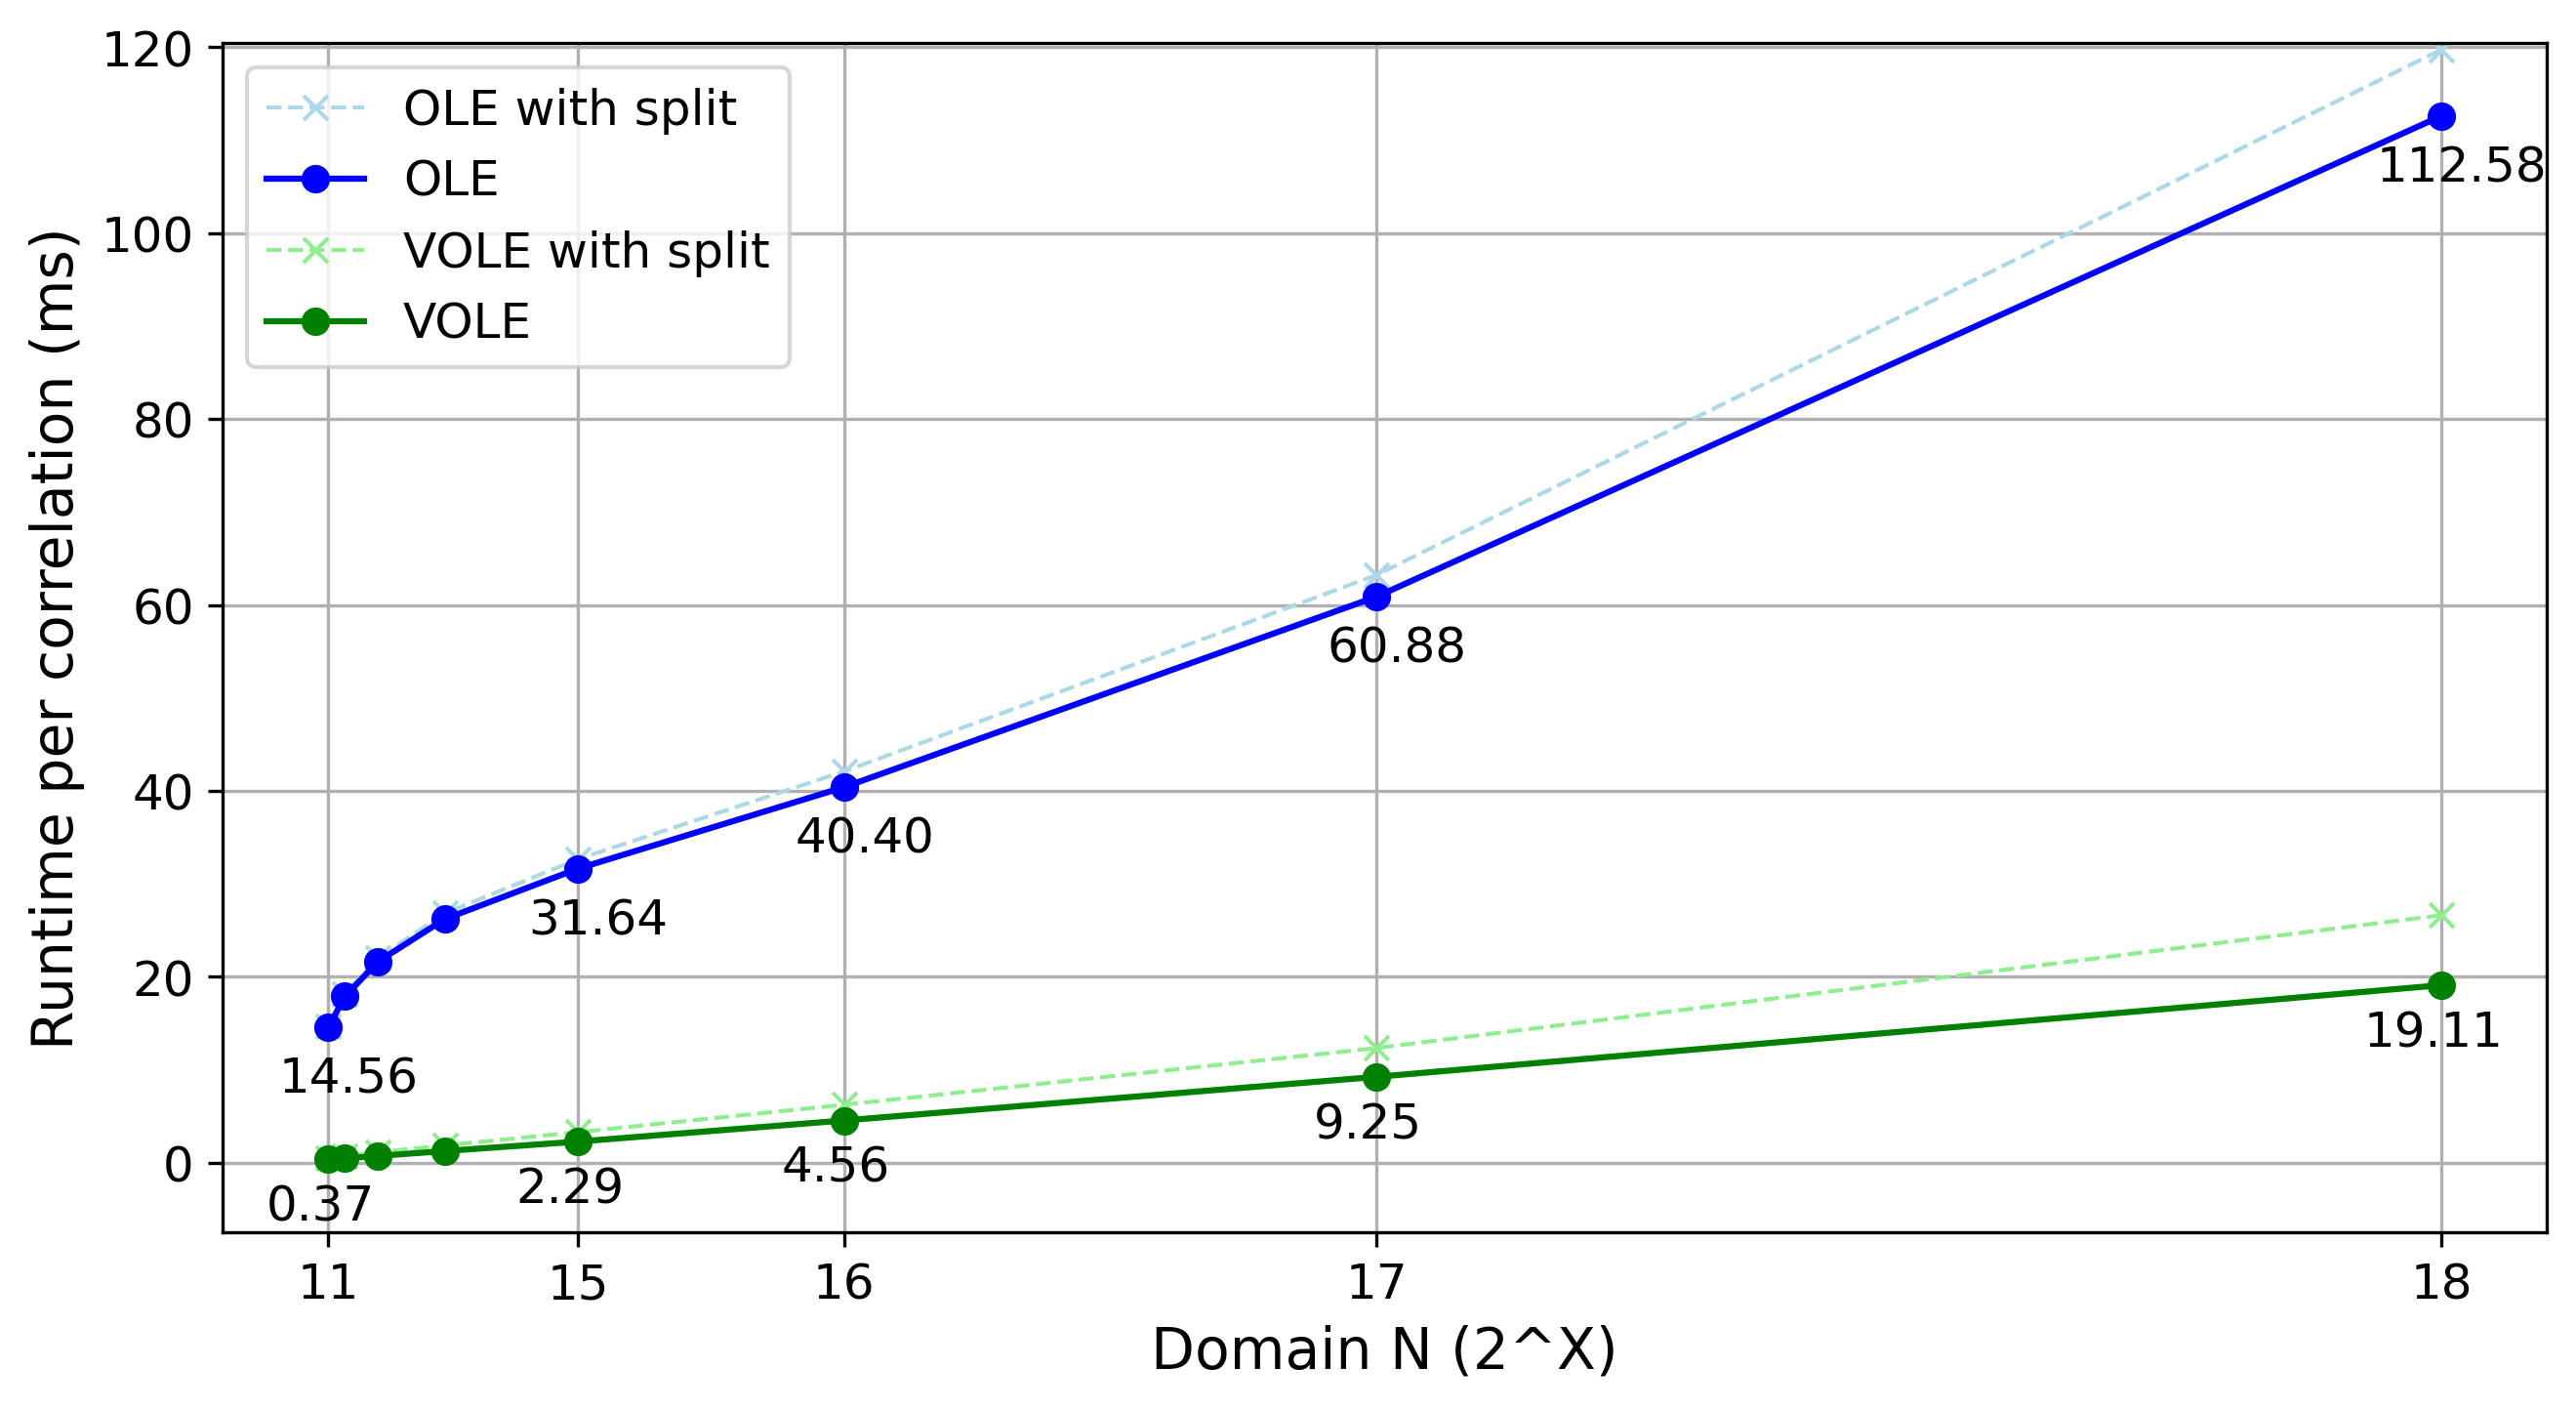
\includegraphics[scale=0.49]{images/plots/pcg_eval.png}
    \caption{Runtime comparison of the PCG expansion for OLE and VOLE over $N$}
    \label{fig:ComparingPCGExpansion}
\end{figure}

\textbf{Splitting the Ring:} Note that the (V)OLE constructions do not include the splitting of the ring elements. However, since this is a crucial practical step, we include the overhead it introduces in Figure \ref{fig:ComparingPCGExpansion} separately. Our parallelized optimizations of Horner's method for polynomial evaluation yield noticeable benefits, resulting in a moderate overhead for the constructions. At $N=2^{18}$, the increase is 39.35\% for VOLE and only 6.34\% for OLE. While the absolute runtime for this operation is identical in both cases, the proportional increase is higher for the VOLE construction due to its lower overall runtime. Therefore, we find that further optimizations would be valuable, particularly to reduce the overhead associated with ring splitting in the VOLE case.
\\\\
\textbf{Full Domain Evaluation:} Processing DSPF full domain evaluations contributes significantly to the overall runtime of the OLE construction, with less of an impact on the VOLE construction. This is analogous to the PCG seed generation described in Section \ref{subsec:evalGen}. Observe the following for LPN-Parameters $(c,\tau)=(4,16)$:
\begin{itemize}
\item OLE Construction: Employs 16x \texttt{DSPF$^{\tau^2}_{2N}$.FullEval}, which implies 4096 DPF full domain evaluation on domain $2N$.
\item VOLE Construction: Utilizing 4x \texttt{DSPF$^{\tau}_{N}$.FullEval}, which implies only 64 DPF full domain evaluation on (smaller) domain $N$.
\end{itemize}
This disparity, coupled with the higher frequency of polynomial multiplication, provides a clear explanation for the longer runtime and worse scaling of the OLE construction. Although we observe these attributes, we believe that the quasilinear performance of both constructions is practical and present an application in Chapter \ref{chapter:PCGforBBSPlus}.
\\\\
\textbf{Profiling:} We suggested that FFT-based polynomial multiplications are the primary runtime bottleneck of the PCG constructions. Although this is indeed the case for large $N$, we found that the (relative) impact of the FFT varies and applies differently on the OLE and VOLE construction. To quantify this behavior, we profile the runtime distribution between generating ring elements (where FFT is used) and the DSPF full domain evaluations in Figure \ref{fig:runtimeAllocationComparision}. We observe that for the OLE construction, the quasilinearity of the FFT becomes dominant only for larger $N$. This is also due to the fact that the runtime required for the (large) DSPF full domain evaluations is quite high to begin with, which is less the case for the smaller DSPF domains in the VOLE case as described before. Simultaneously, this is the reason why the FFT is more dominant for smaller $N$ in the VOLE construction. Recall from Section \ref{subsec:evalDspfFullDomain} that the advantage of parallelizing the full domain evaluation for the OLE case increases with larger $N$ compared to the VOLE case. We recognize this effect here, as the increase in the dominance of the FFT increases steadily for OLE, but flattens out for VOLE. Ultimately, the quasilinear nature of the FFT implies that its relative share of the runtime will approach 100\% in both constructions if $N$ is large enough.

\begin{figure}[t]
    %\centering
    \hspace{-1em}
    \begin{subfigure}[b]{0.5\textwidth}
        \centering
        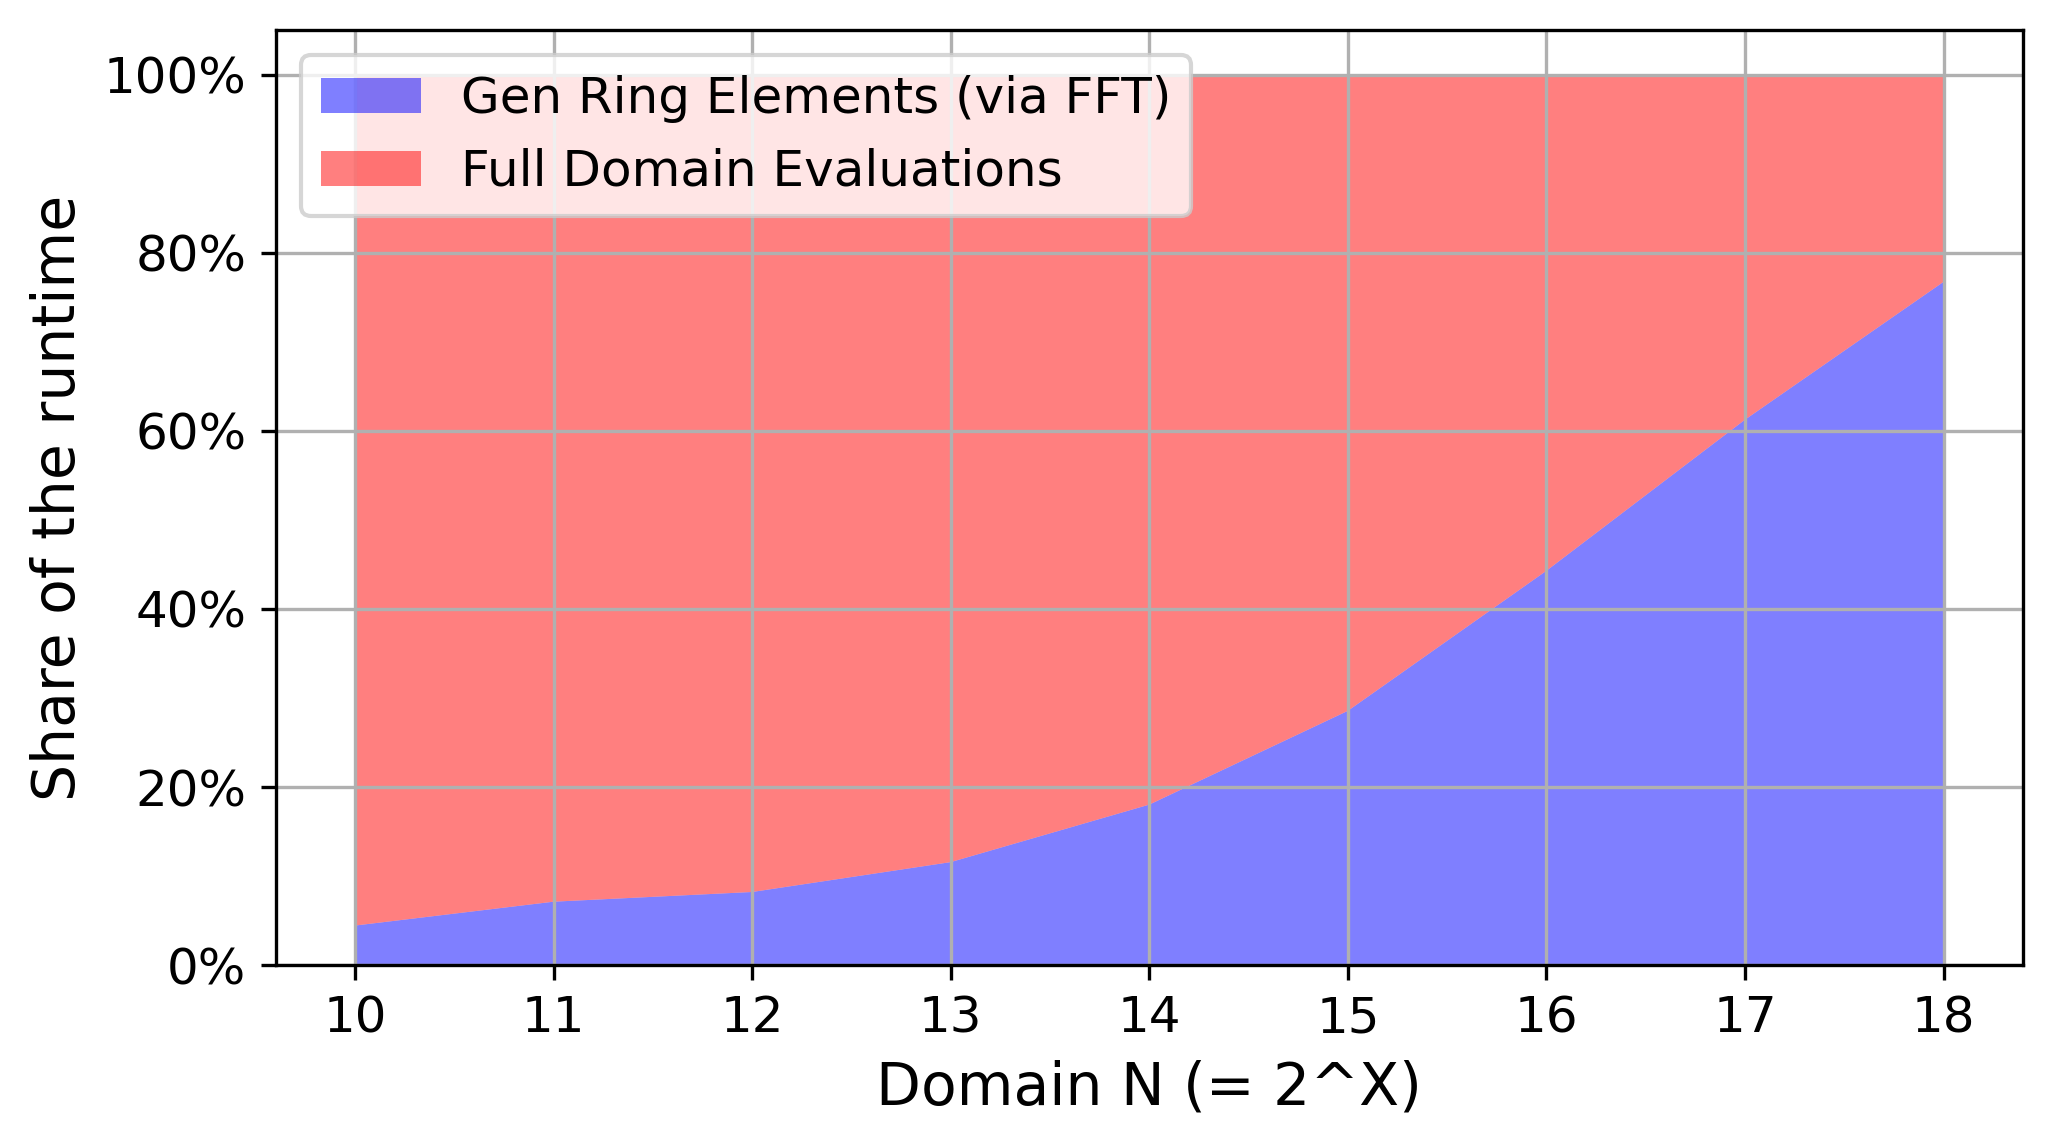
\includegraphics[scale=0.49]{images/plots/ole_percentage_dist.png}
        \caption{OLE construction}
    \end{subfigure}
    \hspace{0em}
    \begin{subfigure}[b]{0.5\textwidth}
        \centering
        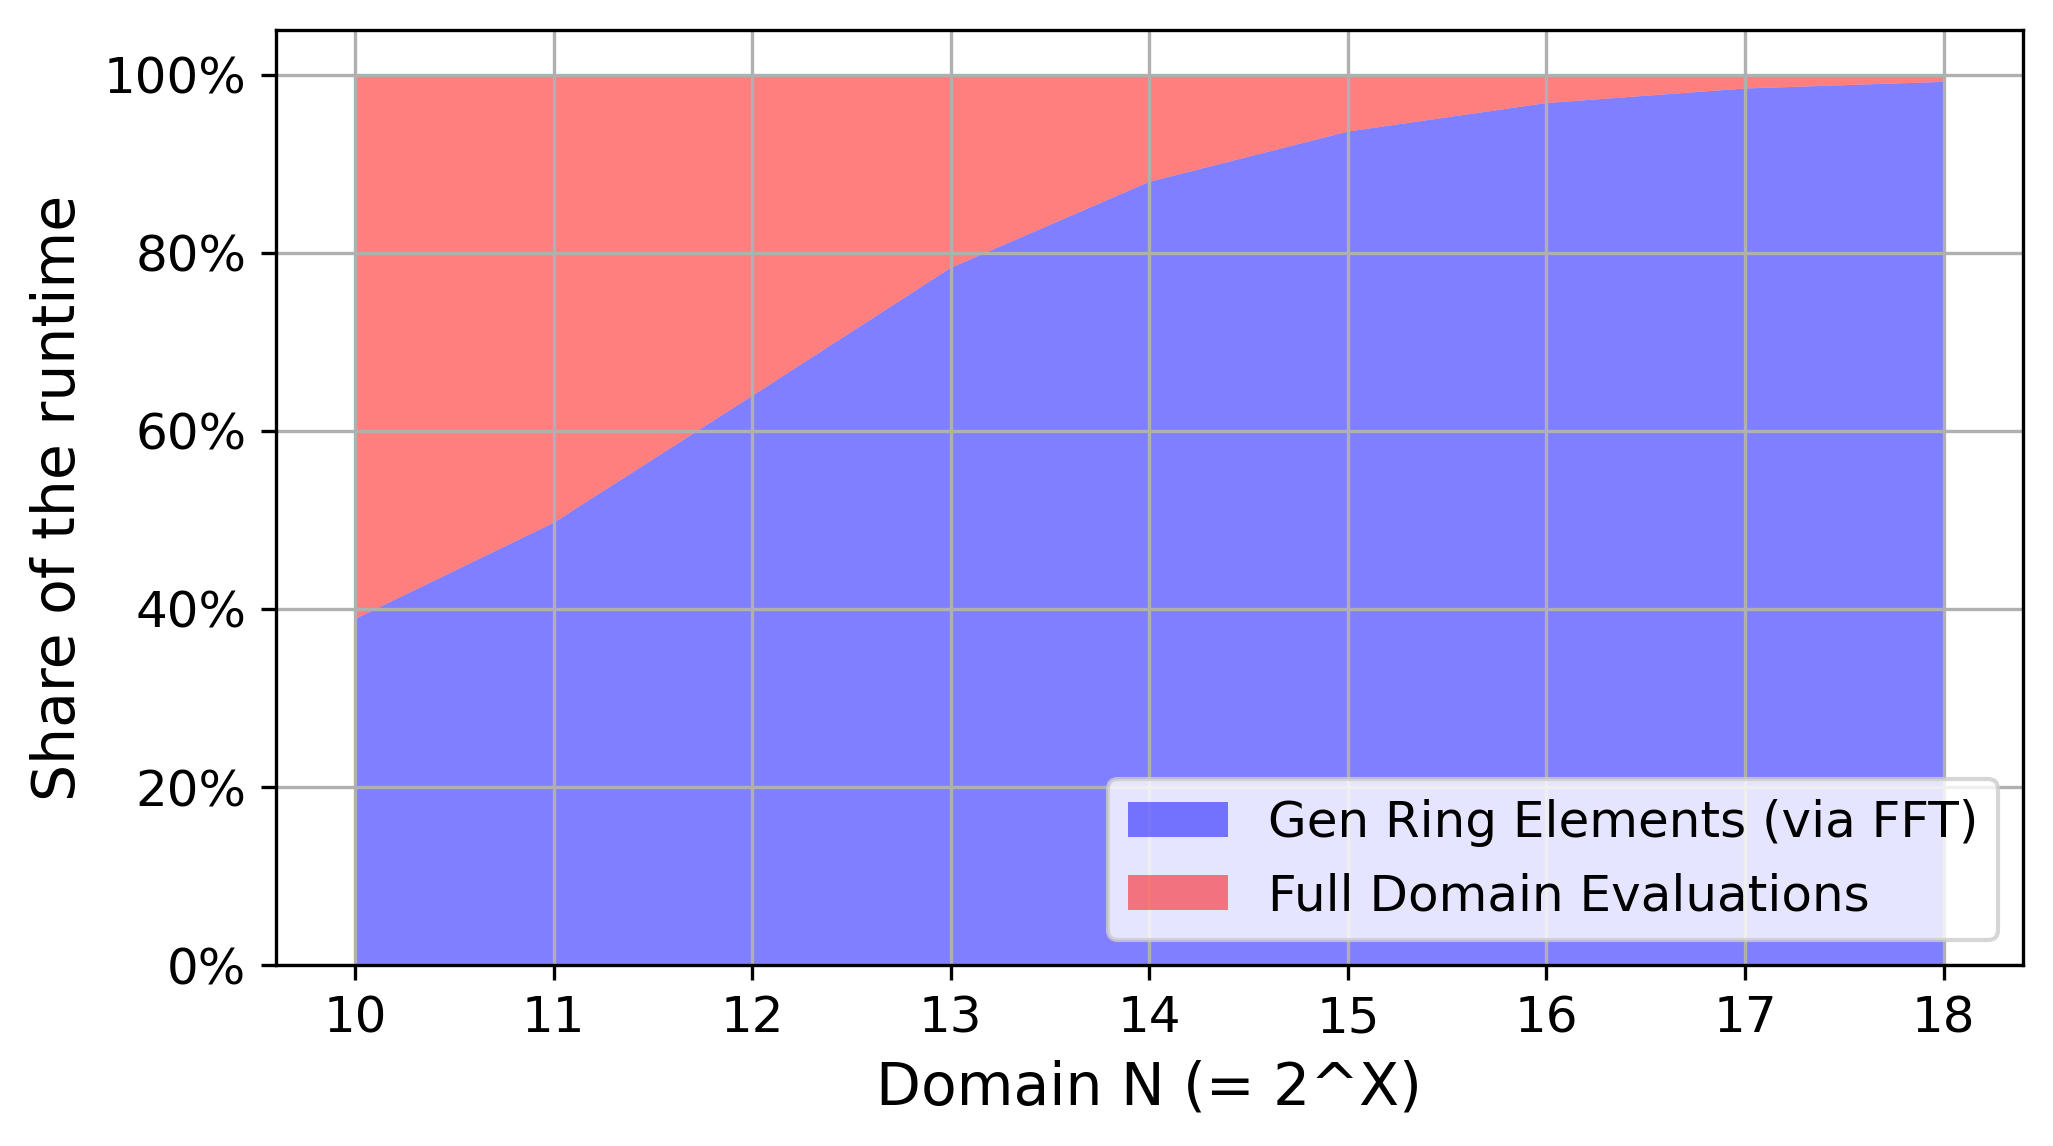
\includegraphics[scale=0.49]{images/plots/vole_percentage_dist.png}
        \caption{VOLE construction}
    \end{subfigure}
    \caption{Comparing runtime allocation of \texttt{PCG.Expand} over $N$}
    \label{fig:runtimeAllocationComparision}
\end{figure}


        \chapter{PCG for Threshold BBS+}
In this chapter, we recall and evaluate an application for PCGs in regard to realizing a threshold signature scheme (Definition \ref{def:tss}) based on BBS+ (Construction \ref{definition:bbs+}). Recent threshold BBS+ schemes \cite{gennaro2019fully, doerner2023threshold} necessitate interaction among parties during signing, resulting in communication overhead that leads to latency, especially in scenarios where the signing parties are geographically dispersed. Faust et al. \cite{cryptoeprint:2023/1076} address this limitation with a threshold BBS+ scheme that strategically divides the signing process into two phases: an interactive \textit{offline} preprocessing phase generating message-independent presignatures and a non-interactive \textit{online} signing phase where presignatures are used without further communication between signers. Besides achieving sublinear communication complexity in the offline phase, the essential advantage of this approach is the trade-off it offers. Shifting computationally demanding operations to the offline phase enables a highly efficient online signing process. This flexibility is beneficial for real-world applications that deal with variable utilization patterns and/or geographically dispersed parties, allowing presignature generation during low-demand periods to then enable rapid signature creation during peak system load. 
\\\\
We begin by recalling the threshold BBS+ scheme by Faust et al. \cite{cryptoeprint:2023/1076}. We explain how the scheme thresholdizes standard BBS+ to achieve applicability of PCGs, such that their expansion enables the offline preprocessing phase. Then, we present a complete construction for the $n$-out-of-$n$ case based on the PCG for (V)OLE from Section \ref{sec:construction}. Further, we show the necessary adaptions to realize the threshold $\tau$-out-of-$n$ case. Finally, we implement both cases, provide benchmarks to evaluate the construction, and derive implications for the efficiency of the online phase. 

\section{Thresholdization}
Refer to Construction \ref{definition:bbs+} for the standard BBS+ signature scheme. For simplicity, we focus on the $n$-out-of-$n$ scenario. Therefore, the key generation (\texttt{\textup{KeyGen}}) can be distributed via additive secret sharing. For an $\tau$-out-of-$n$ scenario, Shamir's Secret Sharing  \cite{shamir1979share} (which employs Lagrange interpolation) would be utilized. Notice that for adapting the signing (\texttt{\textup{Sign}}), the main difficulty lies in distributing the computation of Equation \ref{eq:BBS+standardA}.

\begin{equation}
A := \left( g_1\cdot h_0^s\cdot \prod_{\ell \in [k]} h_{\ell}^{m_{\ell}} \right)^{\frac{1}{x+e}}.
\label{eq:BBS+standardA}
\end{equation}

For realizing the non-interactive online phase, the thresholdization must be able to create message-independent presignatures for $A$ while preventing the disclosure of the secret key (shares of) $x$ during the computation of the inverse of $(x+e)$. This challenge is similar to those faced in other signature schemes that depend on exponentiation, such as ECDSA. Commonly, solving this involves calculating and revealing a value $B = M^a$ and $\delta = a\cdot x$ for a randomly chosen blinding value $a$. The signature of the massage $M^{1/x}$ can then be computed through $B$ without revealing $x$, since $M^{1/x} = B^{1/\delta}$. This is suitable for message-independent presignatures, as $\delta$ remains independent of $M$. This idea is applied in the following:
\\\\
\textbf{BBS+ presignature tuples.} For a $n$-out-of-$n$ setting, secret key $x$ and random blinding factor $a$, we define a BBS+ presignature $\varphi_i$ held by party $P_i$ as a tuple $(a_i,e_i,s_i,\delta_i,\alpha_i) \in \mathbb{Z}^5_q$, such that the following correlations hold

\begin{equation}
\begin{array}{l}
\delta=\sum\limits_{i \in[n]} \delta_i=a(x+e), \quad
\sum\limits_{i \in[n]} \alpha_i=as, \\
a=\sum\limits_{i \in[n]} a_i, \quad e=\sum\limits_{i \in[n]} e_i, \quad s=\sum\limits_{i \in[n]} s_i.
\end{array}
\label{eq:req_correlations}
\end{equation}

Assuming the existence of BBS+ presignature tuples $\varphi_i$, we recall the following $n$-out-of-$n$ TSS:

\begin{construction}[\textbf{$n$-out-of-$n$ Threshold BBS+}]
\label{construction:noutofnTRBBSPlus}
Extending from Construction \ref{definition:bbs+}, let $P_0, \ldots, P_{n-1}$ denote the parties involved, each holding an array of $N$ independent presignatures $\varphi_{i}[1], \ldots, \varphi_{i}[N]$ for party $P_i$. The $n$-out-of-$n$ BBS+ TSS includes the following polynomial-time algorithms:
\begin{itemize}
    \item \texttt{\textup{ThreshKeyGen($1^\lambda$)}}: For a security parameter $\lambda$, sample a secret $x \stackrel{\$}{\leftarrow} \mathbb{Z}_p^*$, compute $y = g_2^x$, and split $x$ as shares ${sk_0, \ldots, sk_{n-1}}$ via a secret sharing scheme. Each party $i$ receives $(pk, sk_i)$.
    \item \texttt{\textup{ThreshSig$_{\varphi_{i}[j]}$($\{m_{\ell}\}_{\ell \in [k]}$)}}: Given secret share $sk_i$ and the \(j\)-th pre-signature $\varphi_{i}[j] = (a_i,e_i,s_i,\delta_i,\alpha_i)$, compute $A_i = h_0^{\alpha_i} \cdot \left( g_1\prod_{\ell \in [k]} h_{\ell}^{m_{\ell}} \right)^{a_i}$ and return partial signature $\sigma_i = (A_i, \delta_i, e_i, s_i)$.
    
    \item \texttt{\textup{CombineSig($\{\sigma_{i}\}_{i \in [n]}$)}}: Combine all partial parital signatures $\{\sigma_{i}\}_{i \in [n]}$ by reconstructing $\delta, e, s$ additively and computing $A = (\prod_{i \in [n]} A_i)^{\frac{1}{\delta}}$ to output $\delta = (A, e, s)$.
    
    \item \texttt{\textup{Verify}}$_{pk}$$(\{m_{\ell}\}_{\ell \in [k]}, \sigma)$: Parse the signature $\sigma = (A, e, s)$ and public key $pk = y$ to output 1 iff $e(A, y \cdot g_2^e) = e(g_1\cdot h_0^s \cdot \prod_{\ell \in [k]} h_{\ell}^{m_{\ell}}, g_2)$.
\end{itemize}
\end{construction}

We observe that \texttt{\textup{CombineSig}} produces a tuple $(A, e, s)$ that represents a valid BBS+ signature as shown in Equation \ref{eq:thresholdBBSplusCorrectness}. Notice that the blinding factor $a$ cancels out. Therefore, the original \texttt{\textup{Verify}} functionality of BBS+ outputs $1$.

\begin{equation}
    A = (\prod_{i \in [n]} A_i)^{\frac{1}{\delta}} = \left( h_0^{as}\cdot (g_1\cdot \prod_{\ell \in [k]} h_{\ell}^{m_{\ell}})^a \right)^{\frac{1}{a(x+e)}} = \left( g_1\cdot h_0^{s}\cdot \prod_{\ell \in [k]} h_{\ell}^{m_{\ell}} \right)^{\frac{1}{x+e}}
\label{eq:thresholdBBSplusCorrectness}  
\end{equation}

Intuitively, the scheme fulfills the \textit{unforgability} property of a TSS (Section \ref{prelim:thresholdSignatures}) as long as no $j$th round of presignatures $\varphi_{0}[j], \ldots, \varphi_{n-1}[j]$ for $j \in [N]$  is used more than once. On the one hand, $a$ and therefore also $\alpha$ and secret $x$ cannot be derived from any (set of) partial signature $\sigma_i$. On the other hand, if each $j$th round of presignatures is independent of any other round $r$ for $r \neq j$ an adversary cannot learn anything from observing valid (partial) signatures.

\section{Offline Preprocessing Phase}
We recalled the construction of a non-interactive $n$-out-of-$n$ BBS+ TSS from \cite{cryptoeprint:2023/1076}, assuming the existence of a message-independent presignature database that satisfies two criteria: (1) each set of presignatures satisfies the specified correlations (cf. Equation \ref{eq:req_correlations}), and (2) each set is computationally indistinguishable from all others so that forgery of unused (partial) presignatures is not possible. These are attributes a PCG (Definition \ref{def:PCGprelim}) can fulfill, as it can securely produce pseudorandom distributions that are correlated in some pre-defined way. Criteria (1) follows from the PCGs \textit{correctness} property, and criteria (2) from the PCGs \textit{security} property.
\\\\
\textbf{Correlations.} Notice that the correlations of BBS+ presignature tuples can be decomposed into two OLE and one VOLE correlation. Specifically, the correlation $\alpha = as$ can be realized as an OLE correlation by assuming that $a$ and $s$ are already additively shared among the parties. Each party $i$, for $i, j \in [n]$, then receives shares of the cross-terms $a_is_j$ (for $i \neq j$) represented as  $a_is_j = z_{(i,j)}^i+z_{(i,j)}^j$. Here, $z_{(i,j)}^i$ denotes the share held by party $i$ and $z_{(i,j)}^j$ denotes the share held by party $j$. Note that party $i$ can compute the term $a_is_i$ locally. Finally, each party $i$ can construct its additive share of $\alpha = \sum_{i\in [n]}\alpha_i$ as in Equation \ref{eq:additiveShareAlpha}:

\begin{equation}
  \alpha_i=a_is_i + \sum_{j \in [n]\backslash \{i\}}{z_{(i,j)}^i} + \sum_{j \in [n]\backslash \{i\}}z_{(j,i)}^i.
  \label{eq:additiveShareAlpha}
\end{equation}

This also works for the other correlations. Notice, that $\delta = a(x+e)$ can be split into an OLE correlation $\delta^0 = ae$ and a VOLE correlation $\delta^1 = ax$, where the secret $x$ is invariant, allowing us to express $\delta$ as the sum $\delta = \delta^0 + \delta^1$. Since there are no other requirements, we can utilize the PCG constructions for (V)OLE correlations introduced in Section \ref{sec:construction} to construct a PCG for BBS+ presignature tuples.

\subsection{PCG Construction for BBS+}
The basic idea behind combining the (V)OLE constructions of Section \ref{sec:construction} for connecting multiple correlations is that we let the individual PCG instantiations share LPN error vectors strategically. Simultaneously, the LPN error vectors themselves can be utilized as additive shares of $a$, $e$, and $s$. We present the PCG construction for BBS+ presignature tuples (Equation \ref{eq:req_correlations}) in Construction \ref{construction:PCGforBBS+}. Our construction is derived from the PCG proposed by Abram et al. \cite{abram2022low} for their non-interactive threshold ECDSA scheme.
\\\\
\textbf{Seed Generation.} For PCG.Gen$_{\texttt{BBS+}}$, we begin with sampling additive secret key shares $sk_i$. We also sample LPN error vectors for every party. Each set of error vectors represents a seed for an additive share of the targeted base parameter $a \sim (\boldsymbol{\omega}, \boldsymbol{\beta})$, $e \sim (\boldsymbol{\eta}, \boldsymbol{\gamma})$, $s \sim (\boldsymbol{\phi}, \boldsymbol{\epsilon})$. In step 3, we initiate the VOLE PCG, for which $sk_i$ serves as the constant parameter. Notice that we multiply the $j$th parties secret share $sk_j$ with $\boldsymbol{\beta}_i$ as we realize a secret share for all cross-term $a_i\cdot sk_j$. For $a_i\cdot sk_i$ a distribution is unnecessary as party $i$ holds all necessary parts. In step 4, we initiate the PCG for OLE for all cross-terms. Notice here how the LPN error vectors of $a$, $(\boldsymbol{\omega}, \boldsymbol{\beta})$ are used for both initiations. This embeds to the relation of the correlations ($\delta_0 = a\cdot e$ and $\alpha = a\cdot s$) the individual PCGs can be expanded for. Ultimately, the seeds that include the party's respective secret key share, the LPN error vectors, and the DSPF keys are returned.
\\\\
\textbf{Seed Expansion.} For PCG.Expand$_{\texttt{BBS+}}$, we begin by reconstructing the LPN error polynomials from the seed. In step 2, each party computes its share of the VOLE correlation by adding its known adjacent term with all shares of the cross-terms. Notice that both directions of the cross-terms need to be evaluated from the DSPF. Similarly, in step 3, the OLE correlations are being evaluated. All parameters are then interpreted as vectors of polynomials. Analogusly to the PCG construction for (V)OLE, computing the inner product of those polynomials with public parameter $a$, then yields ring elements in $R_p$ that adheres to the specified correlations. In order to extract individual BBS+ pairs in $\mathbb{Z}_{p}$, the ring elements need to be split via evaluation on a common root of unity as described in Section \ref{subseq:realtiontofx}.

\begin{specialconstruction}{PCG for BBS+ Presignature Tuples}
\label{construction:PCGforBBS+}
\vspace{1em}

Let $\lambda$ be the security parameter, $(t,c)$ the parameters of the $R^c$-LPN$_t$ assumption, and $p$ the modulus. We denote $N$ as the domain of the PCG. Further, let $R_p:=\mathbb{Z}_{p}[X]/(F(X))$ be a ring for a degree $N$ polynomial $F(X) \in \mathbb{Z}_{p}[X]$ and $\boldsymbol{a} = (1, a_2, ..., a_c)$ for $a_2, ...,a_c \in R_p$ be a public input.

\vspace{1em}

\textbf{PCG.Gen$_{\texttt{BBS+}}(1^\lambda)$:}

\begin{algorithmic}[1]
\State Sample key shares $\mathrm{sk}_{i} \stackrel{\$}{\leftarrow} \mathbb{Z}_{p}$ for every $i \in [n]$.
\State For every $i \in [n], r \in [c]$, sample $\boldsymbol{\omega}_{i}^{r}, \boldsymbol{\eta}_{i}^{r}, \boldsymbol{\phi}_{i}^{r} \stackrel{\$}{\leftarrow} [N]^{t}$ and $\boldsymbol{\beta}_{i}^{r}, \boldsymbol{\gamma}_{i}^{r}, \boldsymbol{\epsilon}_{i}^{r} \stackrel{\$}{\leftarrow} [\mathbb{Z}_{p}]^{t}$ uniformly at random.
\State For every $i, j \in [n]$ with $i \neq j, r \in [c]$, compute
\begin{align*}
& \left(U_{i, j}^{r, 0}, U_{i, j}^{r, 1}\right) \stackrel{\$}{\leftarrow} \texttt{DSPF}_{N}^{t}.\texttt{Gen}\left(\mathbbm{1}^{\lambda}, \boldsymbol{\omega}_{i}^{r}, \mathrm{sk}_{j} \cdot \boldsymbol{\beta}_{i}^{r}\right).
\end{align*}
\State For every $i, j \in [n]$ with $i \neq j, r, s \in [c]$, compute
\begin{align*}
& \left(C_{i, j}^{r, s, 0}, C_{i, j}^{r, s, 1}\right)\stackrel{\$}{\leftarrow} \texttt{DSPF}_{2N}^{t^{2}}.\texttt{Gen}\left(\mathbbm{1}^{\lambda}, \boldsymbol{\omega}_{i}^{r} \boxplus \boldsymbol{\eta}_{j}^{s}, \boldsymbol{\beta}_{i}^{r} \otimes \boldsymbol{\gamma}_{j}^{s}\right), \\
& \left(V_{i, j}^{r, s, 0}, V_{i, j}^{r, s, 1}\right) \stackrel{\$}{\leftarrow} \texttt{DSPF}_{2N}^{t^{2}}.\texttt{Gen}\left(\mathbbm{1}^{\lambda}, \boldsymbol{\omega}_{i}^{r} \boxplus \boldsymbol{\phi}_{j}^{s}, \boldsymbol{\beta}_{i}^{r} \otimes \boldsymbol{\epsilon}_{j}^{s}\right).
\end{align*}
\State For every $i \in [n]$, output the seed
\begin{align*}
\kappa_{i} \leftarrow\left(\mathrm{sk}_{i},\left(\boldsymbol{\omega}_{i}^{r}, \boldsymbol{\eta}_{i}^{r}, \boldsymbol{\phi}_{i}^{r}\right)_{r \in [c]},\left(\boldsymbol{\beta}_{i}^{r}, \boldsymbol{\gamma}_{i}^{r}, \boldsymbol{\epsilon}_{i}^{r}\right)_{r \in [c]},\left(U_{i, j}^{r, 0}, U_{j, i}^{r, 1}, C_{i, j}^{r, s, 0}, C_{j, i}^{r, s, 1}, V_{i, j}^{r, s, 0}, V_{j, i}^{r, s, 1}\right)_{\substack{j \neq i \\ r, s \in [c]}}\right).
\end{align*}
\end{algorithmic}

\vspace{1em} % Space before the next part

\textbf{PCG.Expand$_{\texttt{BBS+}}(\sigma, \kappa_\sigma)$:}

\begin{algorithmic}[1]
\State For every $r \in [c]$, define the degree $< N$, $t$-sparse LPN polynomials:
\begin{align*}
u_{i}^{r}(X):= \sum_{l \in [t]} \beta_{i}^{r}[l] \cdot X^{\omega_{i}^{r}[l]}, \quad  v_{i}^{r}(X):= \sum_{l \in [t]} \gamma_{i}^{r}[l] \cdot X^{\eta_{i}^{r}[l]}, \quad  k_{i}^{r}(X):= \sum_{l \in [t]} \epsilon_{i}^{r}[l] \cdot X^{\phi_{i}^{r}[l]}.
\end{align*}
\State For every $r \in [c]$, compute:
\begin{align*}
& \widetilde{u}_{i}^{r} \leftarrow \mathrm{sk}_{i} \cdot u_{i}^{r}+\sum_{j \neq i}\left(\texttt{DSPF}_{N}^{t}.\texttt{FullEval}\left(U_{i, j}^{r, 0}\right)+\texttt{DSPF}_{N}^{t}.\texttt{FullEval}\left(U_{j, i}^{r, 1}\right)\right).
\end{align*}

\State For every $r, s \in [c]$, compute
\begin{align*}
& w_{i}^{r, s} \leftarrow u_{i}^{r} \cdot v_{i}^{s}+\sum_{j \neq i}\left(\texttt{DSPF}_{2N}^{t^{2}}.\texttt{FullEval}\left(C_{i, j}^{r, s, 0}\right)+\texttt{DSPF}_{2N}^{t^{2}}.\texttt{FullEval}\left(C_{j, i}^{r, s, 1}\right)\right), \\
& m_{i}^{r, s} \leftarrow u_{i}^{r} \cdot k_{i}^{s}+\sum_{j \neq i}\left(\texttt{DSPF}_{2N}^{t^{2}}.\texttt{FullEval}\left(V_{i, j}^{r, s, 0}\right)+\texttt{DSPF}_{2N}^{t^{2}}.\texttt{FullEval}\left(V_{j, i}^{r, s, 1}\right)\right).
\end{align*}

\State Define the vectors of polynomials $\boldsymbol{u}_{i} := (u_{i}^{0}, \ldots, u_{i}^{c-1})$, and similarly for $\boldsymbol{v}_{i}$, $\boldsymbol{k}_{i}$, and $\widetilde{\boldsymbol{u}}_{i}$.

\State Let $\boldsymbol{w}_{i} := (w_{i}^{0,0}, \ldots, w_{i}^{c-1,0}, w_{i}^{0,1}, \ldots, w_{i}^{c-1,1}, \ldots, w_{i}^{c-1, c-1})$, and similarly for $\boldsymbol{m}_{i}$.

\State Compute the final polynomials
\begin{align*}
a_{i} & \leftarrow \left\langle\boldsymbol{a}, \boldsymbol{u}_{i}\right\rangle, & 
s_{i} & \leftarrow \left\langle\boldsymbol{a}, \boldsymbol{v}_{i}\right\rangle, &
e_{i} & \leftarrow \left\langle\boldsymbol{a}, \boldsymbol{k}_{i}\right\rangle, \\
\alpha_{i} & \leftarrow \left\langle\boldsymbol{a} \otimes \boldsymbol{a},  \boldsymbol{w}_{i}\right\rangle, & 
\delta_{i}^{0} & \leftarrow \left\langle\boldsymbol{a} \otimes \boldsymbol{a},  \boldsymbol{m}_{i}\right\rangle, & 
\delta_{i}^{1} & \leftarrow \left\langle\boldsymbol{a},  \widetilde{\boldsymbol{u}}_{i}\right\rangle, \\
& & & & \delta_{i} & \leftarrow \delta_{i}^{0} + \delta_{i}^{1}
\end{align*}
in $\mathbb{F}_{q}[X] / (F(X))$. Output $\left(\alpha_{i}, \mathrm{sk}_{i}, a_{i}, s_{i}, e_{i}, \delta_{i}\right)$.
\end{algorithmic}
\end{specialconstruction}



\subsubsection{Expansion Complexity}
Although the BBS+ presignature tuples only contain two OLE and one VOLE correlation, the presented PCG primitives for (V)OLE (cf. Section \ref{sec:construction}) realize these correlations for two parties. Therefore, we would need to instantiate significantly more primitives for additional parties; each new party requires additional cross-terms. Naively, for $n$ parties, the PCG for BBS+ would consist of $n^2-1$ individual VOLE PCGs and $2\cdot(n^2-1)$ OLE PCGs. This suggests a potentially quadratic scaling. However, notice that Construction \ref{construction:PCGforBBS+} intertwines the individual primitives. Recall from Section \ref{subsec:evalExpansionVOLE} that generating ring elements dominates the runtime in the (V)OLE PCG, especially for large $N$. By directly summing the full domain evaluations (step 2/3), we mitigate this to generate only five ring elements (step 6), independent of the number of parties ($n$). Since ring element generation involves superlinear FFT while full domain evaluations are linear, our construction's overall complexity remains superlinear with respect to the domain size $N$. For $n$ on the other hand, we notice that each additional party adds six full domain evaluations to the expansion. Therefore, Construction \ref{construction:PCGforBBS+}'s computational complexity is superlinear for domain $N$, and linear for the participating parties $n$. Section \ref{sec:evalBBSPlusPCG} provides a detailed evaluation of how this complexity transfers to the implementation.

\subsection{Threshold Setting}
\label{subsec:tauoutofnSetting}
In particular, the summation of the full domain evaluations in step 2/3 hinders compatibility with the $\tau$-out-of-$n$ setting, for threshold $\tau < n$. In this setting, parties require only specific cross-term subsets determined by the current signer set. Direct summation prevents this selective use. Furthermore, summing all cross-terms together impedes interpolation on secret key shares when employing methods like Shamir's Secret Sharing \cite{shamir1979share}.  
\\\\
\textbf{Solution.} We can solve this by individually computing the full domain evaluations and generating a ring element (via $a$) for each. This allows parties to evaluate only the needed ring elements and subsequently interpolate the secret shares according to the signer set. Finally, they can combine all parts to obtain a valid BBS+ tuple. Note that each full domain evaluation must be stored individually for the VOLE component (step 2). However, the forward and backward evaluations can be summed directly in the OLE case (step 3) since interpolation isn't required there. This solution does come with drawbacks. First, there is increased storage overhead since all intermediate results (in form or additional ring elements) need to be retained. Second, computational overhead arises during the expansion due to the need of generating significantly more ring elements (one for each cross-term). We analyze the severity of these computational drawbacks in the following section. Note that, depending on the signer set, the ring elements can be recombined before being split. Therefore, there is no overhead at this point, except for a few (negligible) additions determined by $\tau$. Otherwise, $\tau$ has no influence on the complexity of this approach.

\section{Evaluation}
\label{sec:evalBBSPlusPCG}
In this section, we evaluate our implementation of the PCG for BBS+ Presignature Tuples presented in Construction \ref{construction:PCGforBBS+}, which realizes the offline pre-processing phase of Faust et al.'s non-interactive threshold BBS+ scheme \cite{cryptoeprint:2023/1076}. We start with the $n$-out-of-$n$ setting and compare its performance over different amounts of parties $n$ and domain choices $N$. Further, we evaluate our implementation of the $\tau$-out-of-$n$ setting. We validate that both settings stay superlinear (regarding domain $N$) driven through FFT for generating the ring elements and that an increase in participating parties only comes with a linear increase in runtime. This behavior implies that the PCG is practical for realizing an offline pre-processing phase for Construction \ref{construction:noutofnTRBBSPlus}. We find that the adaption to the $\tau$-out-of-$n$ setting strengthens the superlinearity of the approach, therefore only introducing a manageable overhead. Furthermore, we identify areas of improvement and verify the efficiency of the implementation by comparing our runtimes to \cite{abram2022low}. Finally, we recall the assessment of the online phase from \cite{cryptoeprint:2023/1076} and apply findings of our evaluation.
\\\\
\textbf{Setup.} We employ the same benchmarking setup previously introduced in Chapter \ref{chapter:evaluation}, utilizing a Xeon Gold 5120 CPU @ 2.20GHz with 14 cores and 64GB of RAM. We maintain the optimizations and parallel processing techniques discussed in Chapter \ref{chapter:ImplementingPCGs} and again choose LPN parameters $(c,t)=(4,16)$, as suggested by Boyle et al. \cite{boyle2020efficient}. Because of the complexity of the benchmarks and the large number of repetitions within the constructions, we limit our benchmark execution to a single run for each parameter configuration.

\subsection{$n$-out-of-$n$}
We evaluate our implementation of the $n$-out-of-$n$ setting for parties $n\in \{2, ..., 10\}$ and domains $N\in \{2^{11}, ...,2^{19}\}$ in Figure \ref{fig:BBSnoutofn}. As expected, we observe a superlinear runtime increase with respect to the domain size $N$ for all party counts. Concurrently, runtime increases linearly for $n$. This aligns with our complexity analysis:

\begin{itemize}
    \item \textbf{Ring Element Generation:} The generation of ring elements is independent of $n$ and fixed while contributing a superlinear runtime increase for $N$ due to the use of FFT. Therefore, we observe that the runtime increase over $N$ is similar for all $n$.
    \item \textbf{Full Domain Evaluations:} The amount of full domain evaluations scales linearly with $n$, while each instantiation comes with linear complexity (cf. Section X). Therefore, we observed a linear increase in runtime per additional participant.
\end{itemize}

Compared to the reported runtimes for the original PCG for OLE (recall Figure \ref{fig:ComparingPCGExpansion}), our BBS+ construction achieves a disproportionately favorable runtime, even though it handles multiple correlations (2x OLE, 1x VOLE). Focusing on the two-party case for a fair comparison, a single BBS+ tuple requires $100$ms at $N=2^{17}$, while a single OLE correlation takes roughly $60$ms. This highlights the effectiveness of intertwining the PCG primitives.

\begin{figure}[t]
    \centering
    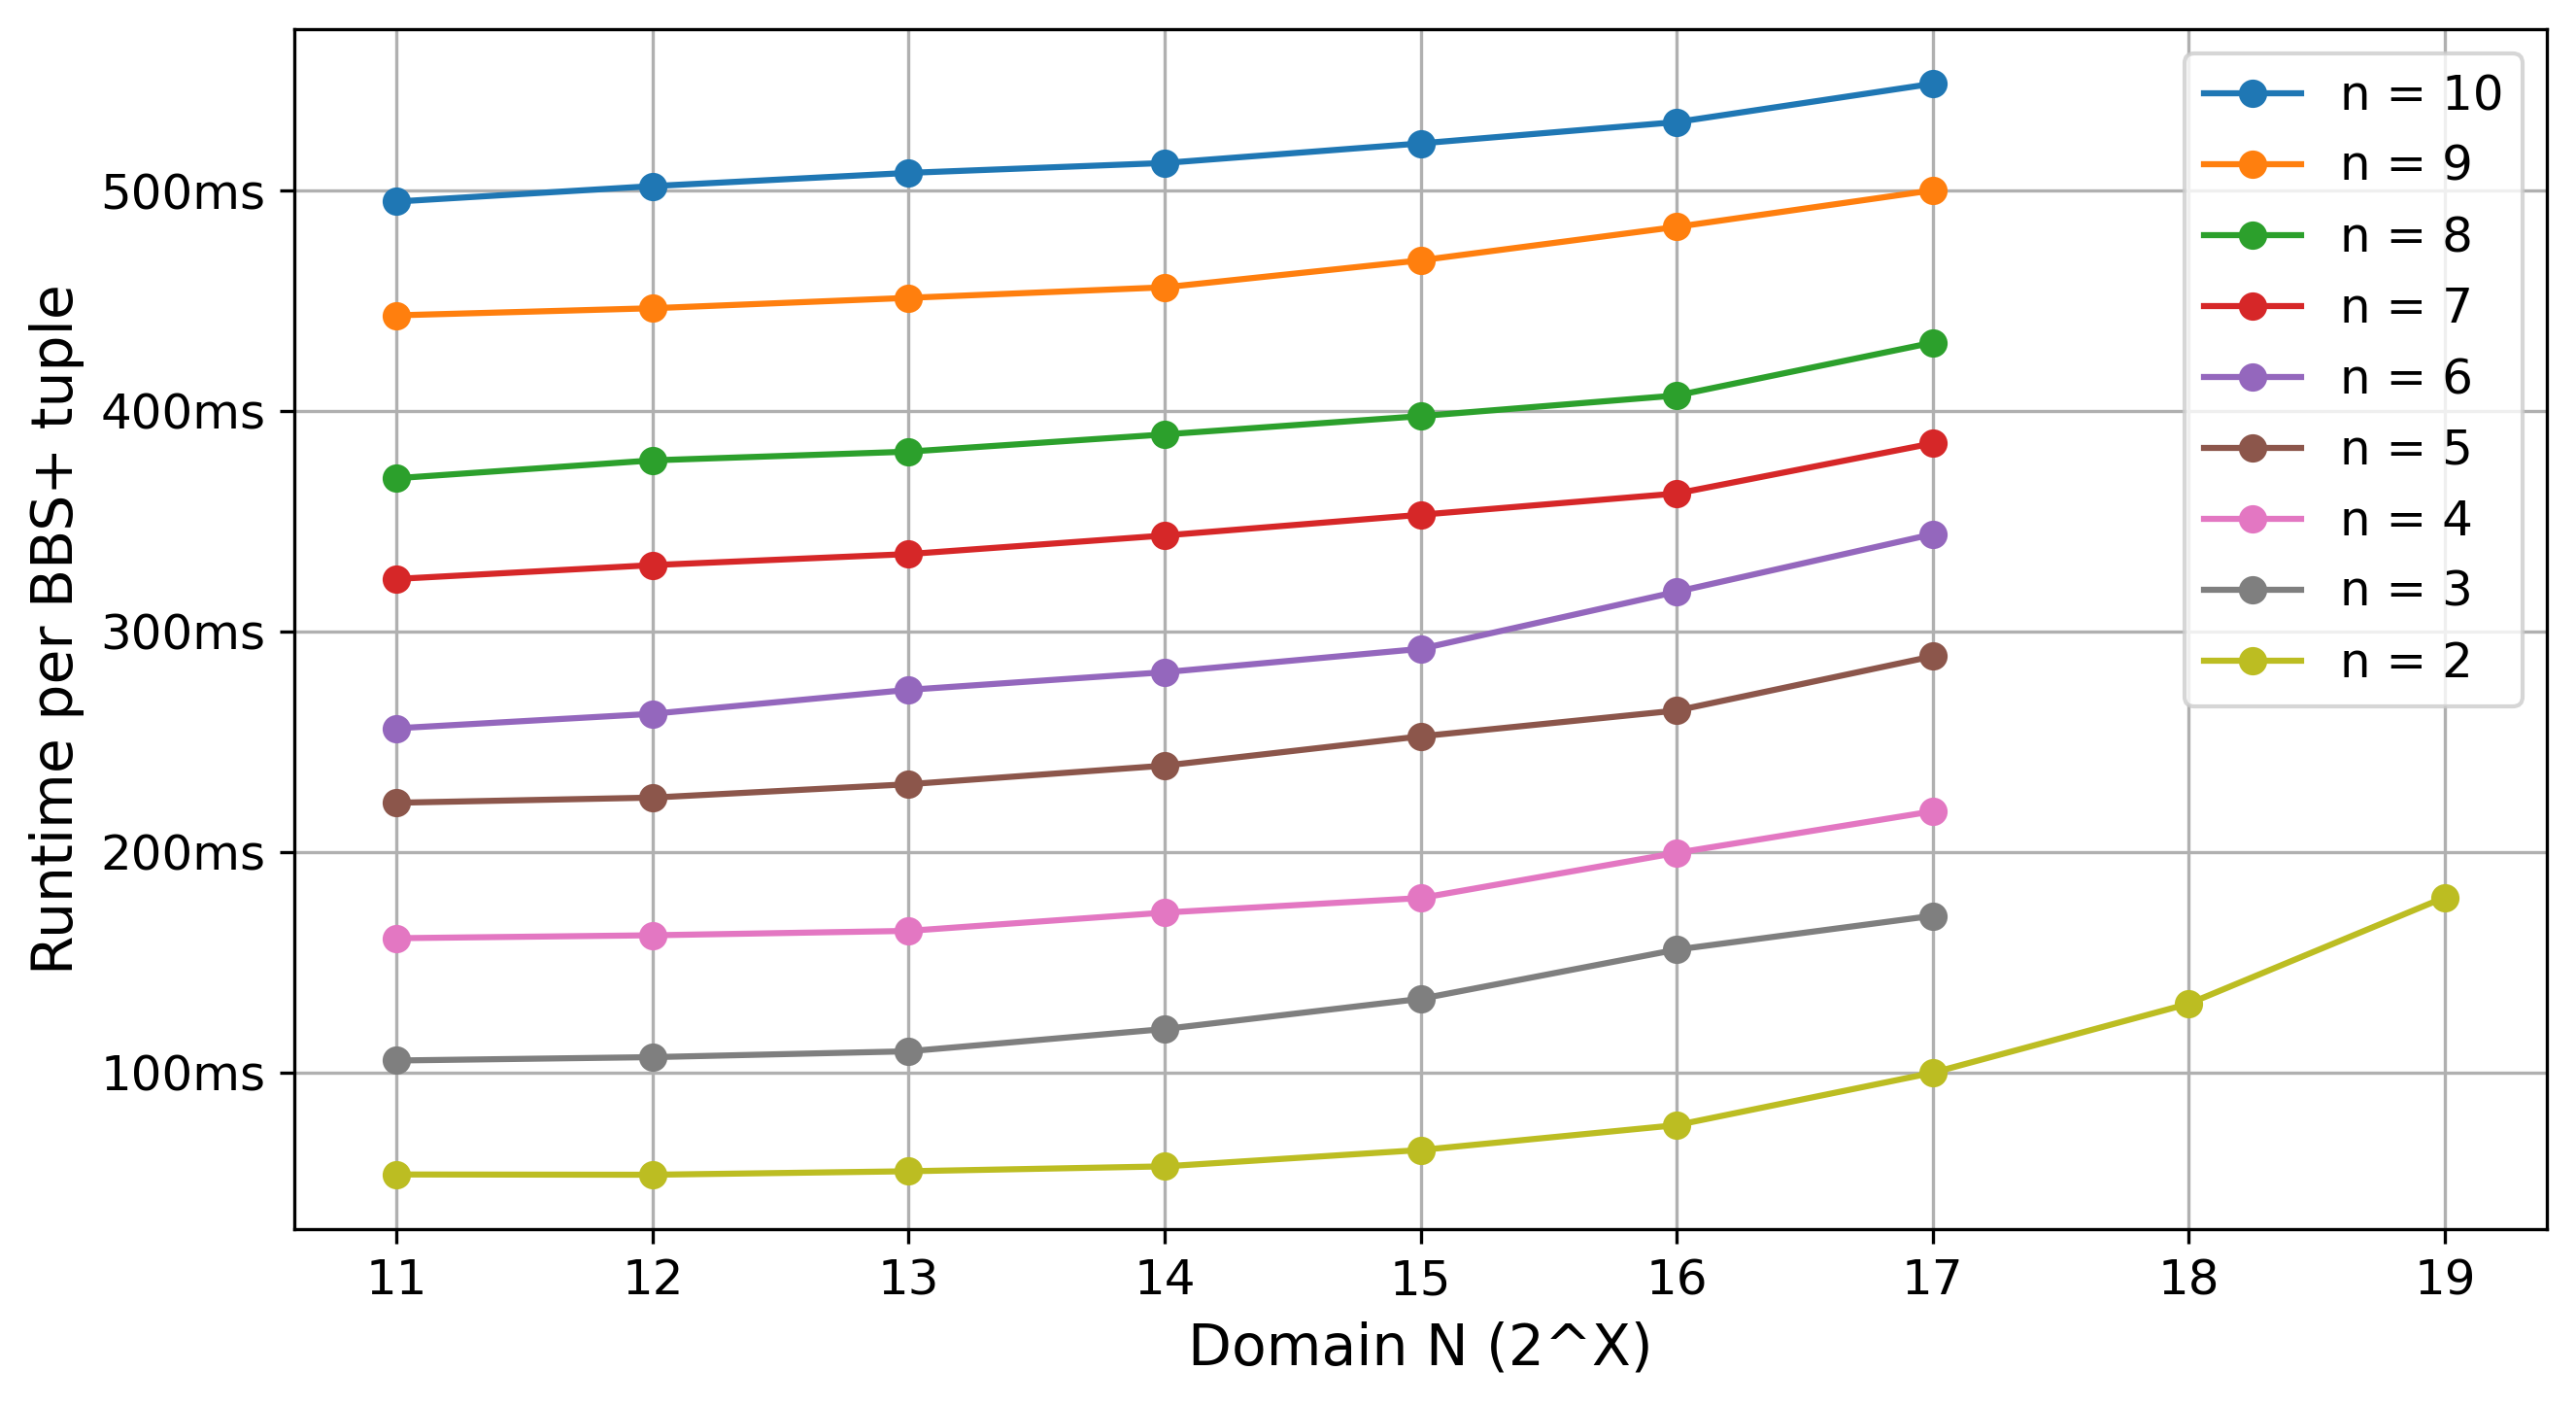
\includegraphics[scale=0.49]{images/plots/bbs_pcg_NoutofN.png}
    \caption{$n$-out-of-$n$ BBS+ PCG expansion over $N$}
    \label{fig:BBSnoutofn}
\end{figure}

\subsection{$\tau$-out-of-$n$}
We evaluate our implementation of the $\tau$-out-of-$n$ setting for $\tau = 2$, parties $n\in \{3, ..., 10\}$ and domains $N\in \{2^{11}, ...,2^{18}\}$ in Figure \ref{fig:BBSnoutofn}. Notably, $\tau$ does not influence the runtime as described in Section \ref{subsec:tauoutofnSetting}; therefore, the presented numbers hold for any choice of $\tau$. Again, we observe that the runtime increases superlinear for domain $N$. In contrast to the $n$-out-of-$n$ setting before, the runtime increase over $N$ is notably steeper. This behavior derives from the construction now needing to deal with more ring elements, leading to more frequent use of FFT. Since FFT is used more frequently, the primitive has a higher (non-linear) impact on the total runtime, resulting in a stronger runtime increase over $N$.
\\\\
\textbf{Comparison to $n$-out-of-$n$.} Directly comparing runtimes, we find the $\tau$-out-of-$n$ implementation takes roughly 37\% longer for $2^{17}$ and $n=3$, with similar overhead existing for other values of $n$. This confirms that the presented adaption for realizing the $\tau$-out-of-$n$ setting while introducing some overhead remains computationally manageable.
\\\\
\textbf{Introducing Overhead to the Online Phase.} We observe that one major drawback of the $\tau$-out-of-$n$ approach for Construction \ref{construction:PCGforBBS+} is that we cannot split the ring elements during pre-processing, as the signer set is needed to combine the ring elements accordingly before evaluating them on a specific root of unity. This forces us to perform these operations during the online phase of the threshold BBS+ scheme. Although the amount of ring element evaluations is fixed (to 5), the degree of their polynomial representation is determined by $N$. This implies that choosing larger domains $N$ for the PCG in the offline phase introduces an increasing overhead during the online signing phase. This increase can be quantified as five degree-$N$ polynomial evaluations, therefore by recalling numbers from Figure \ref{fig:polyEvalBench}, the overhead for $N=2^{10}$ amounts to $0.3$ms and $N=2^{18}$ to $18.8$ms. Since the points at which the polynomials need to be evaluated are known in advance, there may be room for improvement since exponentiations could be pre-calculated. In any case, some overhead remains at this stage. We decide to leave this potential optimization as future work.

\begin{figure}[t]
    \centering
    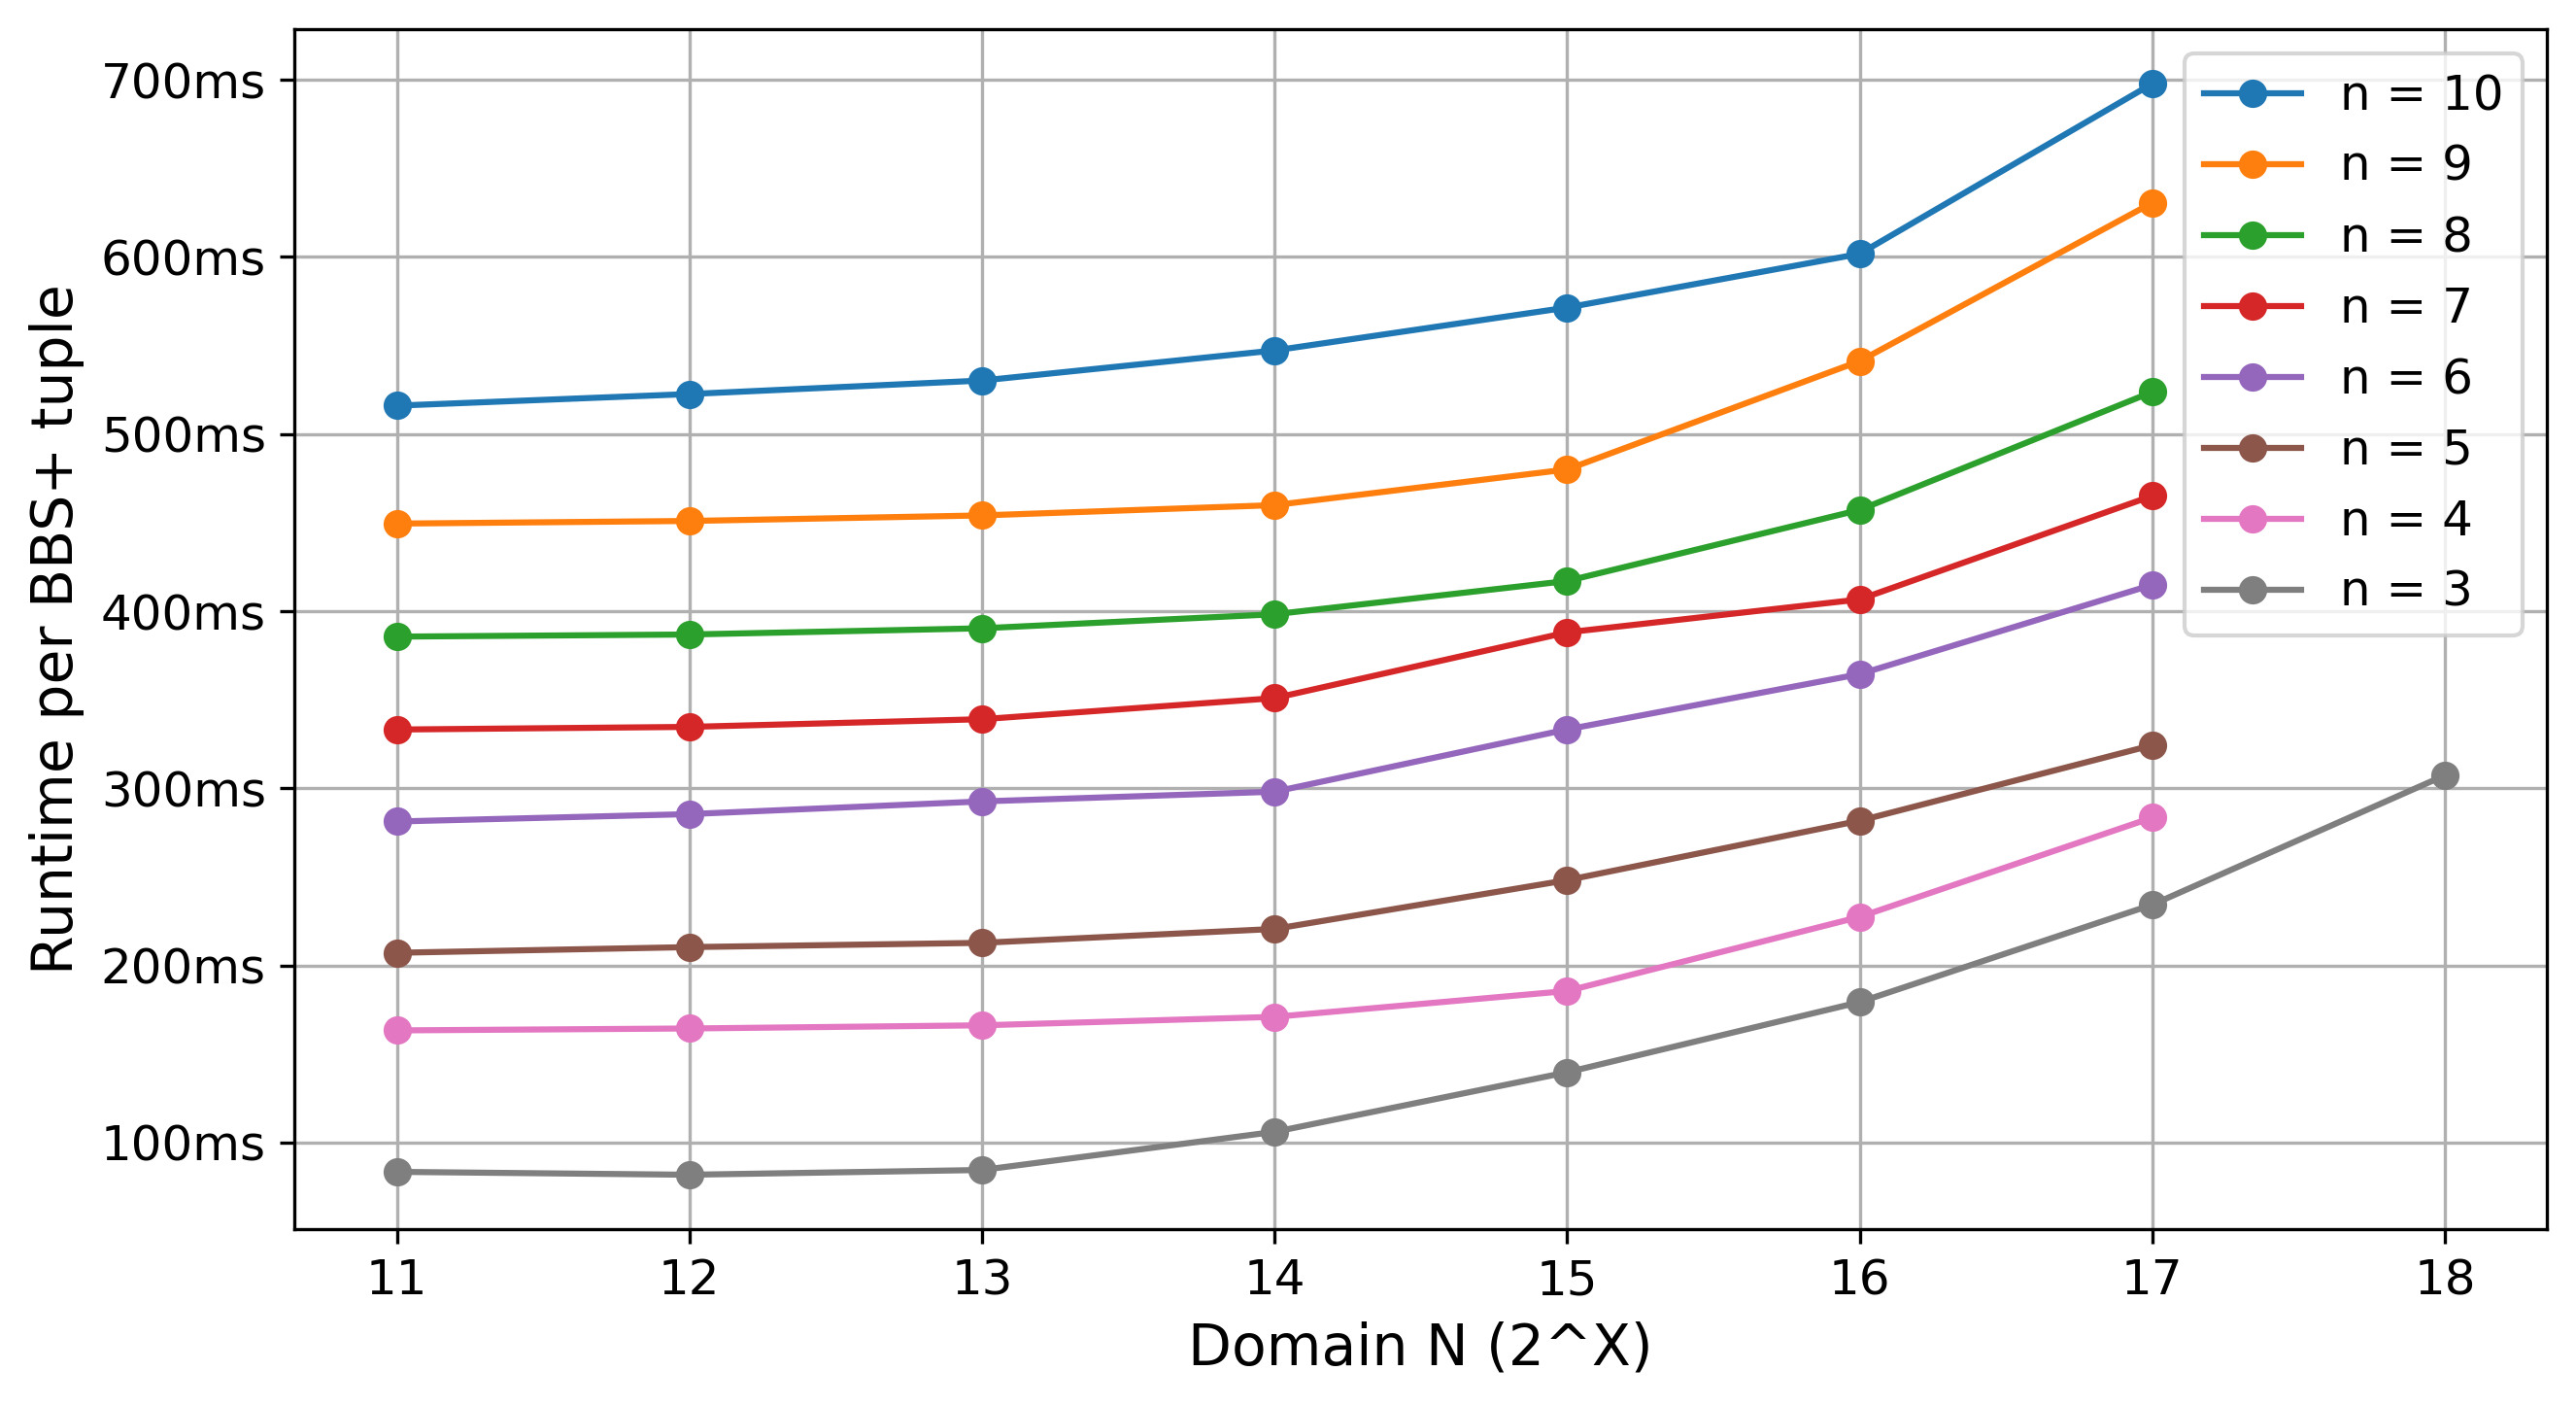
\includegraphics[scale=0.49]{images/plots/bbs_pcg_TAUoutofN.png}
    \caption{$2$-out-of-$n$ BBS+ PCG expansion over $N$}
    \label{fig:BBStauoutofn}
\end{figure}

\subsection{Identifying Bottlenecks}
Recall that in the PCG for (V)OLE, generating ring elements using FFT was the primary performance bottleneck (cf. Figure \ref{fig:runtimeAllocationComparision} ), especially for large domains. However, let us analyze how this changes within the context of the BBS+ PCG. Figure \ref{fig:runtimeAllocationComparision} breaks down the construction's runtime for different party counts ($n$) on $N=2^{17}$.
\\\\
In the $\tau$-out-of-$n$ setting, the proportion of time spent on full domain evaluations versus ring element generation remains roughly constant. This is because as $n$ becomes larger, more full domain evaluations are needed for each of which additional ring elements need to be created. Therefore, the runtime increases similarly for both building blocks, resulting in an allocation that remains close to constant. Interestingly, in the $n$-out-of-$n$ setting, ring element generation becomes less dominant. This trend is expected as the number of ring elements stays fixed while full domain evaluations increase with $n$. Surprisingly, in contrast to FFT being the main cost within the PCG for (V)OLE, our analysis reveals that full domain evaluations of DSPFs represent the primary bottleneck in the PCG for BBS+ Tuples. Therefore, further optimizing this building block would significantly improve the overall performance.
\\\\
\textbf{Comparison to \cite{abram2022low}.}
For evaluating the overall efficiency gains introduced by our practical considerations, we compare our runtimes with the Rust implementation\footnote{\url{https://github.com/ZenGo-X/silent-ecdsa}} of a $n$-out-of-$n$ PCG for threshold ECDSA proposed by Abram et al. in \cite{abram2022low}. Since our construction is derived from theirs, the PCGs are very similar. The main difference is that their PCG incorporates only one OLE and one VOLE correlation, while ours incorporates two OLE and one VOLE. Similar to our implementation, the DSPF building block is parallelized and operates on Boyle et al.'s tree-based approach \cite{boyle2016function}. Therefore, we argue that comparing their implementation to ours is meaningful, although we want to emphasize that Rust generally offers a performance advantage compared to Go in most scenarios\footnote{\url{https://benchmarksgame-team.pages.debian.net/benchmarksgame/fastest/rust-go.html}}. For technical reasons, their selection for the PCG's domain $N$ is not a power of two, but from a given set of optimized values that we adhere to. For a fair comparison, we run their implementation on our test bench and find that for the $2$-out-of-$2$ setting, the PCG requires per pre-signature $247.79$ms for $N=14304$ and $871.83$ms for $N=94019$. These runtimes align (proportionately over $N$) with their reported numbers. From our runtimes (cf. Figure \ref{fig:BBSnoutofn}), we derive that our implementation significantly outperforms theirs by approximately $6$x for the same settings despite generating an additional OLE correlation. Consequently, we conclude that the careful optimizations concerning the building blocks as presented in Chapter \ref{chapter:ImplementingPCGs} contribute significant performance improvements to the overall runtime of \texttt{Module-LPN} based PCGs as introduced by Boyle et al. \cite{boyle2020efficient}, therefore positively affecting their practicality. 

\begin{figure}[t]
    %\centering
    \hspace{-1em}
    \begin{subfigure}[b]{0.5\textwidth}
        \centering
        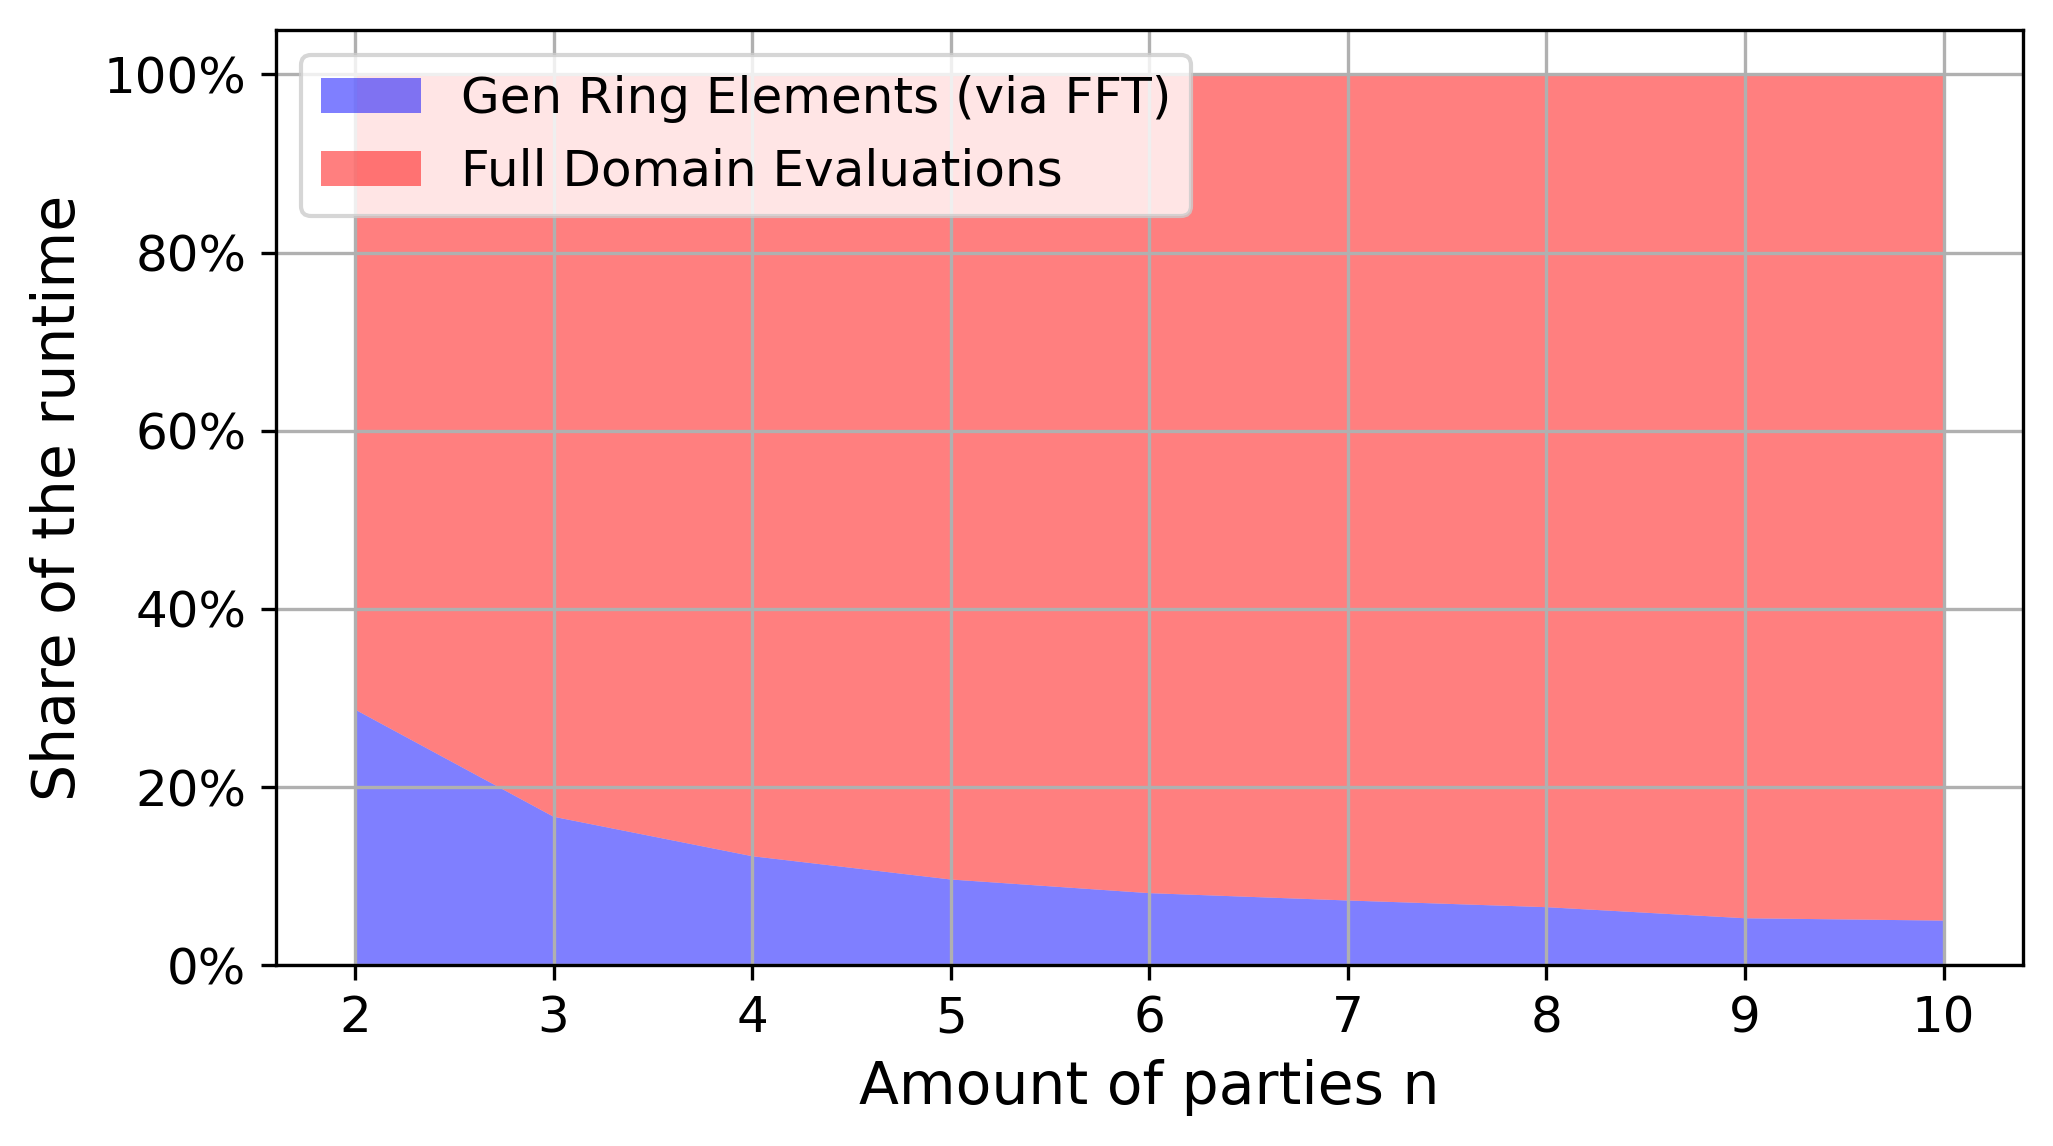
\includegraphics[scale=0.49]{images/plots/bbs_noutofN_percentage_dist.png}
        \caption{$n$-out-of-$n$}
    \end{subfigure}
    \hspace{0em}
    \begin{subfigure}[b]{0.5\textwidth}
        \centering
        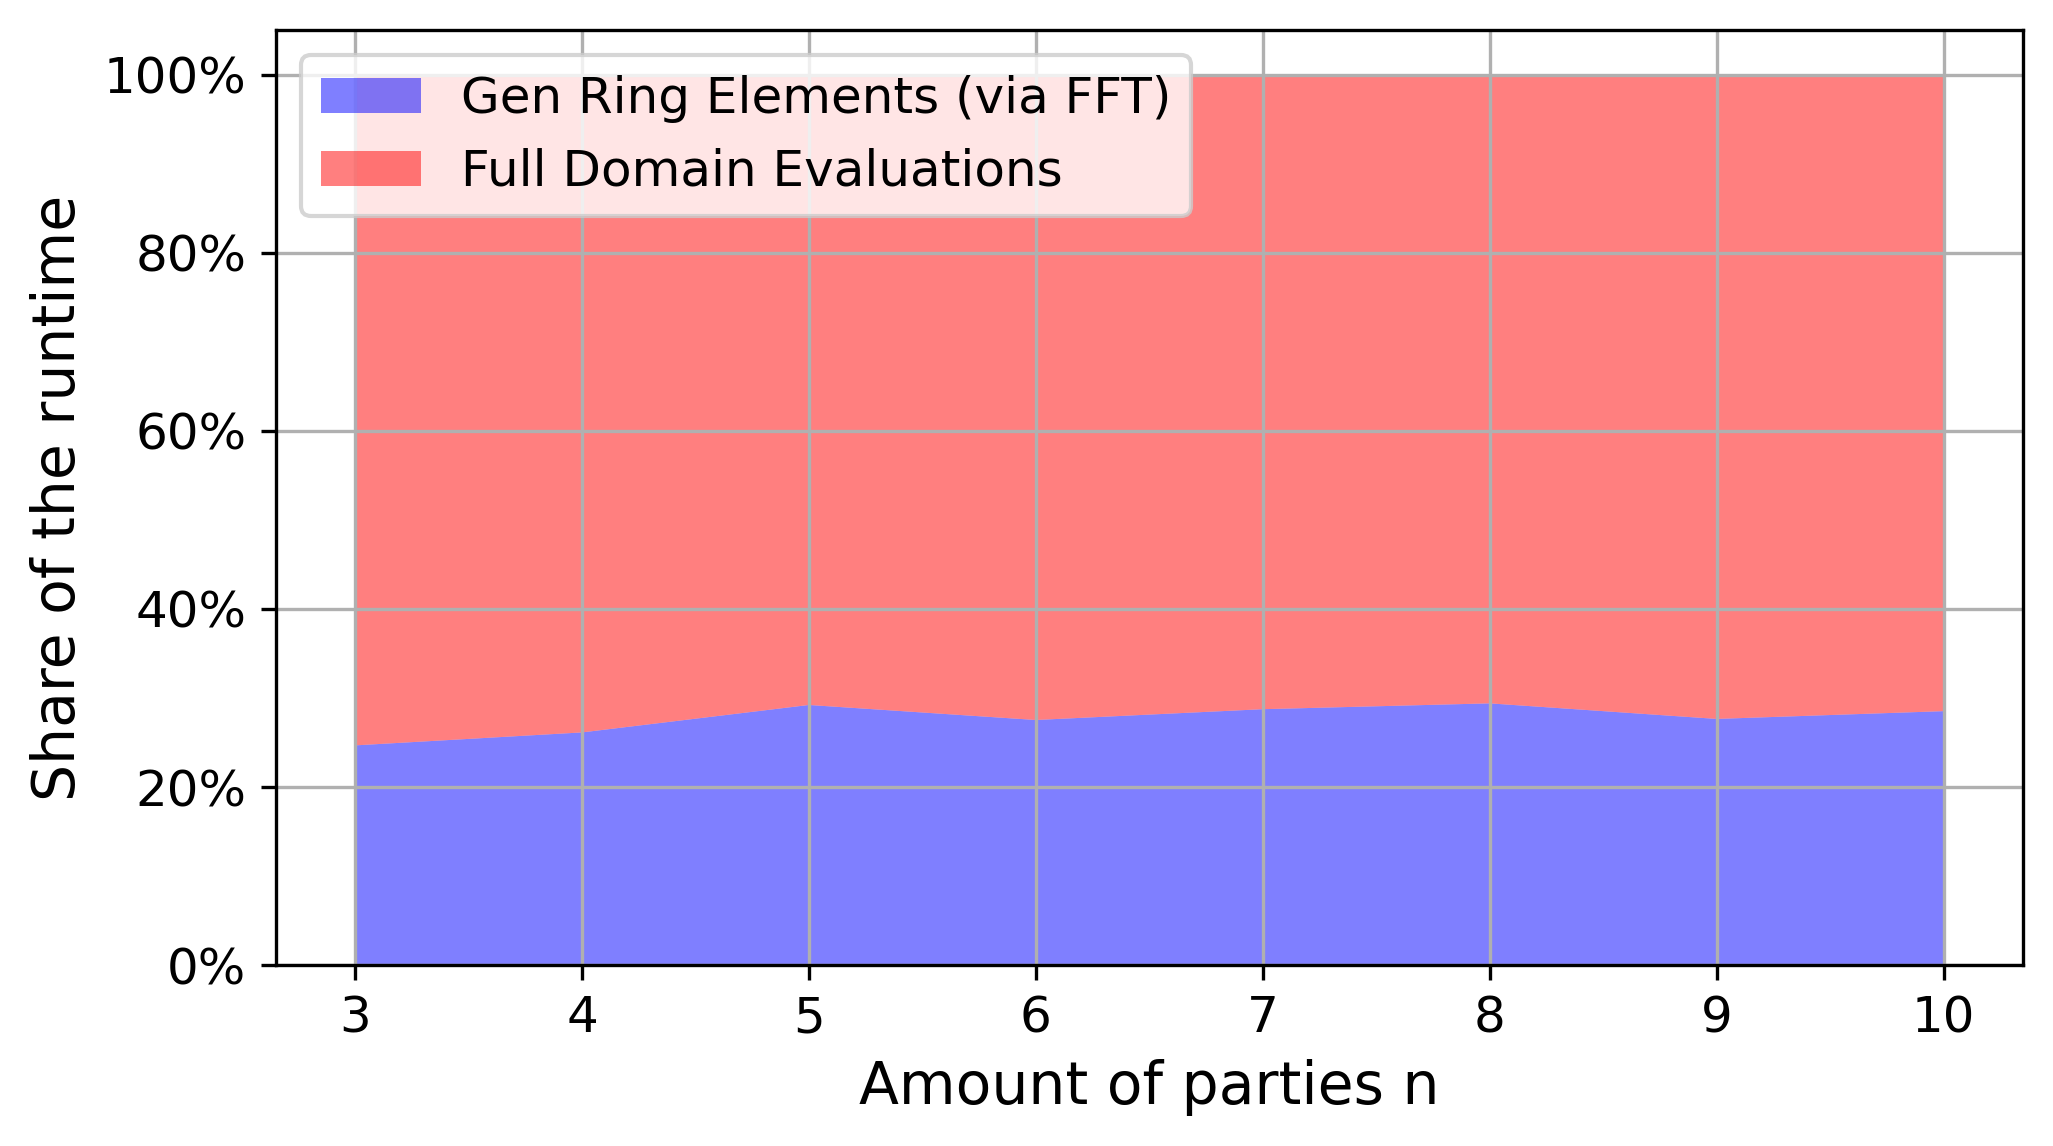
\includegraphics[scale=0.49]{images/plots/bbs_TAUoutofN_percentage_dist.png}
        \caption{$2$-out-of-$n$}
    \end{subfigure}
    \label{fig:runtimeAllocationComparision}
    \caption{Comparing runtime allocation of $n$-out-of-$n$ with $2$-out-of-$n$ for $N=2^{17}$}
\end{figure}

\subsection{Implications for Non-Interactive Threshold BBS+}
The presented benchmarks show that the implemented PCG, while resource intensive, is practical for the offline pre-processing phase of Faust et al.'s threshold BBS+ scheme \cite{cryptoeprint:2023/1076}. For the 2-out-of-2 setting, $2^{17}$ signatures can be pre-processed in around $9.5$ hours (under $132$ms per signature), which is certainly practical for some real-world applications, e.g., when pre-processing is performed overnight. Having generated the pre-signatures, Faust et al. \cite{cryptoeprint:2023/1076} report for the online phase that their implementation of \texttt{ThreshSign} then requires around $0.3$ms per included message $l\in[k]$, with notably no communication needed between the signing parties. Note that communication between the signing parties and the requester must still be accounted for, which makes the server with the highest latency determine the total runtime of the signing protocol. In that regard, Faust et al. compare their online signing phase with an interactive threshold BBS+ protocol by Doerner et al. \cite{doerner2023threshold} that does not employ the preprocessing model. The authors find that the non-interactive approach pays off, especially in the WAN setting, as it achieves between $2$x and $3$x superior runtimes. In the LAN setting, the speedup is increasing linearly over the participating parties, with around $0.5$x for 10 parties to $2$x for 15 parties.
\\\\
While the above evaluation of the online phase holds for the $n$-out-of-$n$ setting, it disregards the overhead the $\tau$-out-of-$n$ setting introduces. Applying the overhead to the reported numbers reveals that this potentially impacts the protocol's advantage in lower latency settings, dependent on the chosen $N$ in the offline phase. Faust et al. report a runtime of around $8$ms for $k=1$ in the LAN setting, constant for the amount of participating parties. As reported, assuming $N=2^{18}$, additional $18.8$ms need to be accounted for. The overhead can be reduced by making $N$ smaller, but this also results in fewer pre-signatures available. Depending on the amount of participating parties (that drive up the runtime in the interactive scheme) and chosen $N$, the non-interactive approach may loose its advantage in the LAN scenario. Note that this is heavily dependent on the chosen parameters and only effects low-latency settings. The advantage of the non-interactive online phase still holds for high latency settings (like WAN), regardless of the number of participating parties. Therefore, in applications where high latency is a dominant factor, the employed preprocessing model offers a clear advantage over interactive approaches, regardless of the chosen threshold.
        
        \chapter{Conclusion}
The central contribution of this thesis is the presentation of practical considerations for implementing Boyle et al.'s \texttt{Ring-LPN} based PCG primitive \cite{boyle2020efficient}. These considerations include the optimization of the underlying DSPF building block for reduced space complexity (Section \ref{sec:dspfImplementation}) and the strategic use of different approaches for handling sparse polynomials (Section \ref{sec:polyOperationsImpl}). We also presented a formula for iteratively computing roots of unity (Section \ref{subseq:realtiontofx}) and show how the principles of Horner's method \cite{horner1819xxi} can be used to compute all roots of unity within linear time complexity (Section \ref{sec:fxconsiderationsImpl}). Evaluations within Chapter \ref{chapter:evaluation} highlight the impact of these optimizations on the practicality of the PCG construction. The PCG implementation derived from the optimized building blocks exhibits quasilinear scaling as the number of correlations generated increases (Section \ref{subsec:evalExpansionVOLE}). This is very appealing for real-world applications that utilize this PCG for preprocessing since the setup phase amortizes faster, and it allows the non-interactive online phase to be longer by mitigating the repetition of the preprocessing phase.
\\\\
To further demonstrate the value of our optimizations, we incorporate the building blocks for implementing the preprocessing phase of Faust et al.'s threshold BBS+ scheme \cite{faust2023non}. Our proposed PCG is optimized for the $n$-out-of-$n$ case (Section \ref{subsec:pcgForBBs+}) and can easily adapt to the threshold setting (Section \ref{subsec:tauoutofnSetting}). Implementations for both cases validate the quasilinear scaling concerning the number of preprocessed correlations (Section \ref{sec:evalBBSPlusPCG}). Notably, the preprocessing phase exhibits linear scaling concerning the number of parties, demonstrating the scheme's suitability for including many signers. Compared to the only other PCG implementation available \cite{abram2022low} (which is limited to the $n$-out-of-$n$ case), our implementation achieves a 6x performance improvement for $n=2$ (Section \ref{subsec:bbspPcgBottlenecks}), clearly highlighting the effectiveness of our practical considerations considering that our PCG includes an additional OLE correlation.
\\\\
Finally, within the $t$-out-of-$n$ threshold case, we acknowledge a limitation of the proposed PCG for threshold BBS+ signature scheme, which introduces a linear overhead in the online phase proportional to the number of precomputed correlations (Section \ref{subsec:implNIBBs+}). We observe that this overhead significantly impacts the protocol runtime in low-latency environments (LAN), while its impact is insignificant in high-latency environments (WAN).

\section{Future Work}
We identify several promising directions for future research. Firstly, Boyle et al. \cite{boyle2020efficient} propose various suitable LPN parameter sets achieving 128-bit security equivalence. While we employed $(c,\tau)=(4,16)$ for consistency with prior work \cite{abram2022low}, evaluating performance across different parameter choices for potentially higher security levels presents an interesting direction for future practical assessment. Secondly, our work primarily addressed PCG expansion, assuming a trusted seed generation phase. Implementing and evaluating the distributed setup phase outlined (but not implemented) by Abram et al. \cite{abram2022low} would be a valuable extension. Furthermore, in Section \ref{subsec:toutofnEval}, we briefly mention the possibility to reduce the overhead introduced within the $t$-out-of-$n$ threshold setting. Optimizations here could mitigate the overhead that the offline phase introduces to the online phase, making the scheme more interesting for low-latency settings as well. Finally, Tessaro et al. \cite{tessaro2023revisiting} recently proposed a more compact BBS+ signature scheme that eliminates the need for one OLE correlation within Faust et al.'s BBS+ presignatures. Investigating the potential performance gains of applying this simplification to the PCG remains future work.
        
	\newpage
    %\bibliographystyle{unsrt}
    %\bibliography{ref}
	\printbibliography
	\appendix
\end{document}